\documentclass[]{article}
\usepackage[T1]{fontenc}
\usepackage{lmodern}
\usepackage{amssymb,amsmath}
\usepackage{ifxetex,ifluatex}
\usepackage{fixltx2e} % provides \textsubscript

%put a newpage before sections http://blog.dreasgrech.com/2010/01/starting-new-page-with-every-section-in.html
\let\stdsection\section
\renewcommand\section{\newpage\stdsection}

% use upquote if available, for straight quotes in verbatim environments
\IfFileExists{upquote.sty}{\usepackage{upquote}}{}
\ifnum 0\ifxetex 1\fi\ifluatex 1\fi=0 % if pdftex
  \usepackage[utf8]{inputenc}
\else % if luatex or xelatex
  \usepackage{fontspec}
  \ifxetex
    \usepackage{xltxtra,xunicode}
  \fi
  \defaultfontfeatures{Mapping=tex-text,Scale=MatchLowercase}
  \newcommand{\euro}{€}
\fi
% use microtype if available
\IfFileExists{microtype.sty}{\usepackage{microtype}}{}
\usepackage{color}
\usepackage{fancyvrb}
\DefineShortVerb[commandchars=\\\{\}]{\|}
\DefineVerbatimEnvironment{Highlighting}{Verbatim}{commandchars=\\\{\}}
% Add ',fontsize=\small' for more characters per line
\newenvironment{Shaded}{}{}
\newcommand{\KeywordTok}[1]{\textcolor[rgb]{0.00,0.44,0.13}{\textbf{{#1}}}}
\newcommand{\DataTypeTok}[1]{\textcolor[rgb]{0.56,0.13,0.00}{{#1}}}
\newcommand{\DecValTok}[1]{\textcolor[rgb]{0.25,0.63,0.44}{{#1}}}
\newcommand{\BaseNTok}[1]{\textcolor[rgb]{0.25,0.63,0.44}{{#1}}}
\newcommand{\FloatTok}[1]{\textcolor[rgb]{0.25,0.63,0.44}{{#1}}}
\newcommand{\CharTok}[1]{\textcolor[rgb]{0.25,0.44,0.63}{{#1}}}
\newcommand{\StringTok}[1]{\textcolor[rgb]{0.25,0.44,0.63}{{#1}}}
\newcommand{\CommentTok}[1]{\textcolor[rgb]{0.38,0.63,0.69}{\textit{{#1}}}}
\newcommand{\OtherTok}[1]{\textcolor[rgb]{0.00,0.44,0.13}{{#1}}}
\newcommand{\AlertTok}[1]{\textcolor[rgb]{1.00,0.00,0.00}{\textbf{{#1}}}}
\newcommand{\FunctionTok}[1]{\textcolor[rgb]{0.02,0.16,0.49}{{#1}}}
\newcommand{\RegionMarkerTok}[1]{{#1}}
\newcommand{\ErrorTok}[1]{\textcolor[rgb]{1.00,0.00,0.00}{\textbf{{#1}}}}
\newcommand{\NormalTok}[1]{{#1}}
\usepackage{longtable}
\usepackage{graphicx}
% We will generate all images so they have a width \maxwidth. This means
% that they will get their normal width if they fit onto the page, but
% are scaled down if they would overflow the margins.
\makeatletter
\def\maxwidth{\ifdim\Gin@nat@width>\linewidth\linewidth
\else\Gin@nat@width\fi}
\makeatother
\let\Oldincludegraphics\includegraphics
\renewcommand{\includegraphics}[1]{\Oldincludegraphics[width=\maxwidth]{#1}}
\ifxetex
  \usepackage[setpagesize=false, % page size defined by xetex
              unicode=false, % unicode breaks when used with xetex
              xetex]{hyperref}
\else
  \usepackage[unicode=true]{hyperref}
\fi
\hypersetup{breaklinks=true,
            bookmarks=true,
            pdfauthor={Jim Higson},
            pdftitle={Oboe.js: An approach to i/o for rest clients which is neither batch nor stream; nor SAX nor DOM},
            colorlinks=true,
            urlcolor=blue,
            linkcolor=magenta,
            pdfborder={0 0 0}}
\urlstyle{same}  % don't use monospace font for urls
\setlength{\parindent}{0pt}
\setlength{\parskip}{6pt plus 2pt minus 1pt}
\setlength{\emergencystretch}{3em}  % prevent overfull lines
\setcounter{secnumdepth}{5}

\title{Oboe.js: An approach to i/o for rest clients which is neither batch nor
       stream; nor SAX nor DOM}
\author{Jim Higson}
\date{2013}

\begin{document}
\maketitle


{
\clearpage
\hypersetup{linkcolor=black}
\setcounter{tocdepth}{3}
\tableofcontents
}

\clearpage
\listoffigures

\clearpage

\section{Abstract}

A new design for http client libraries incorporating http streaming,
pattern matching, and incremental parsing, with the aim of improving
performance, fault tolerance, and encouraging a greater degree of loose
coupling between programs. A Javascript client capable of progressively
parsing JSON resources is presented targeting both Node.js and web
browsers. Loose coupling is particularly considered in light of the
application of Agile methodologies to REST and SOA, providing a
framework in which it is acceptable to partially restructure the JSON
format in which a resource is expressed whilst maintaining compatibility
with dependent systems.

A critique is made of current practice under which resources are
entirely retrieved before items of interest are extracted
programmatically. An alternative model is presented allowing the
specification of items of interest using a declarative syntax similar to
JSONPath. The identified items are then provided incrementally while the
resource is still downloading.

In addition to a consideration of performance in absolute terms, the
usability implications of an incremental model are also evaluated with
regards to developer ergonomics and end user perception of performance.

\section{Introduction}

This purpose of this dissertation is to encourage the REST paradigm to
be viewed through a novel lens which in application this may be used to
deliver tangible benefits to many common REST use cases. Although I
express my thesis through programming, the contribution I hope to make
is felt more strongly as a modification in how we \emph{think} about
http than as the delivery of new software.

In the interest of developer ergonomics, REST clients have tended to
style the calling of remote resources similar to the call style of the
host programming language. Depending on the language, one of two schemas
are followed: a synchronous style in which a some invocation halts
execution for the duration of the request before evaluating to the
fetched resource; or asynchronous in which the logic is specified to be
applied to a response once it is available. Languages encourage our
thinking to follow the terms that they easily support(Whorf 1956). While
there is some overlap, languages which promote concurrency though
threading consider blocking in a single thread to be acceptable and will
generally prefer the former mode whereas languages with first class
functions are naturally conversant in callbacks and will prefer the
latter. We should remember in programming that languages limit the
patterns that we readily see (Yukihiro 2003) and that better mappings
may be possible. This observation extends to graphical notations such as
UML whose constructs strongly reflect the programming languages of the
day. For any multi-packet message sent via a network some parts will
arrive before others, at least approximately in-order, but viewed from
inside a language whose statements invariably yield single, discrete
values it comfortable to conceptualise the REST response as a discrete
event. UML sequence diagrams contain the syntax for instantaneously
delivered return values, with no corresponding notation for a resource
whose data is progressively revealed.

In most practical cases where we wish to be fast in performing a task
there is no reasonable distinction between acting \emph{earlier} and
being \emph{quicker}. To create efficient software we should be using
data at the first possible opportunity: examining content \emph{while it
streams} rather than holding it unexamined until it is wholly available.

While the coining of the term REST represented a shift in how we think
about http, away from the transfer of hypertext documents to that of
arbitrary data (Fielding 2000, 407--416), it introduced no fundamentally
new methods. Similarly building on previous ideas, no new computing
techniques need be invented to realise my thesis. As a minimum it
requires an http client which reveals the response whilst it is in
progress and a parser which can begin to interpret that response before
it sees all of it. Nor is it novel to use these preexisting parts in
composition. Every current web browser already implements such a schema;
load any complex webpage -- essentially an aggregation of hypertext and
other resources -- the HTML will be parsed and displayed incrementally
while it is downloading and resources such as images are requested in
parallel as soon as they are referenced. The images may themselves be
presented incrementally in the case of progressive JPEGs or
SVGs\footnote{For quite an obviously visible example of progressive SVG
  loading, try loading this SVG using a recent version of Google Chrome:
  \url{http://upload.wikimedia.org/wikipedia/commons/0/04/Marriage_(Same-Sex_Couples)_Bill,_Second_Reading.svg}
  For the perfectionist SVG artist, not just the final image should be
  considered but also the XML source order, for example in this case it
  would be helpful if the outline of the UK appeared first and the
  exploded sections last.}. This incremental display is achieved through
highly optimised software created for a single task, that of displaying
web pages. The new contribution of this dissertation is to provide a
generic analog applicable to any problem domain.

\subsection{How REST aggregation could be faster}

\begin{figure}[htbp]
\centering
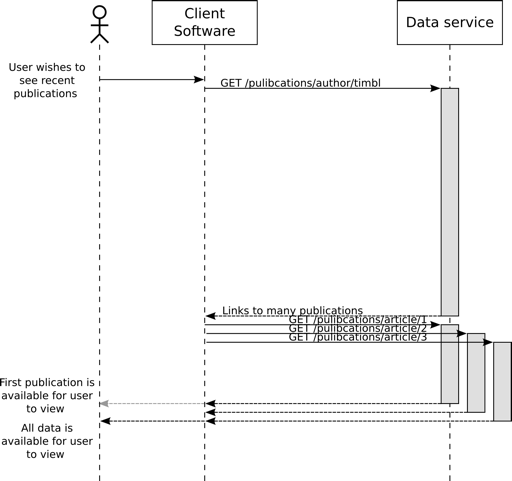
\includegraphics{images/rest_timeline_1.png}
\caption{\textbf{Sequence diagram showing the aggregation of low-level
REST resources.} A client fetches an author's publication list and then
their first three articles. This sequence represents the most commonly
used technique in which the client does not react to the response until
it is complete. In this example the second wave of requests cannot be
made until the original response is complete, at which time they are
issued in quick succession. \label{rest_timeline_1}}
\end{figure}

\begin{figure}[htbp]
\centering
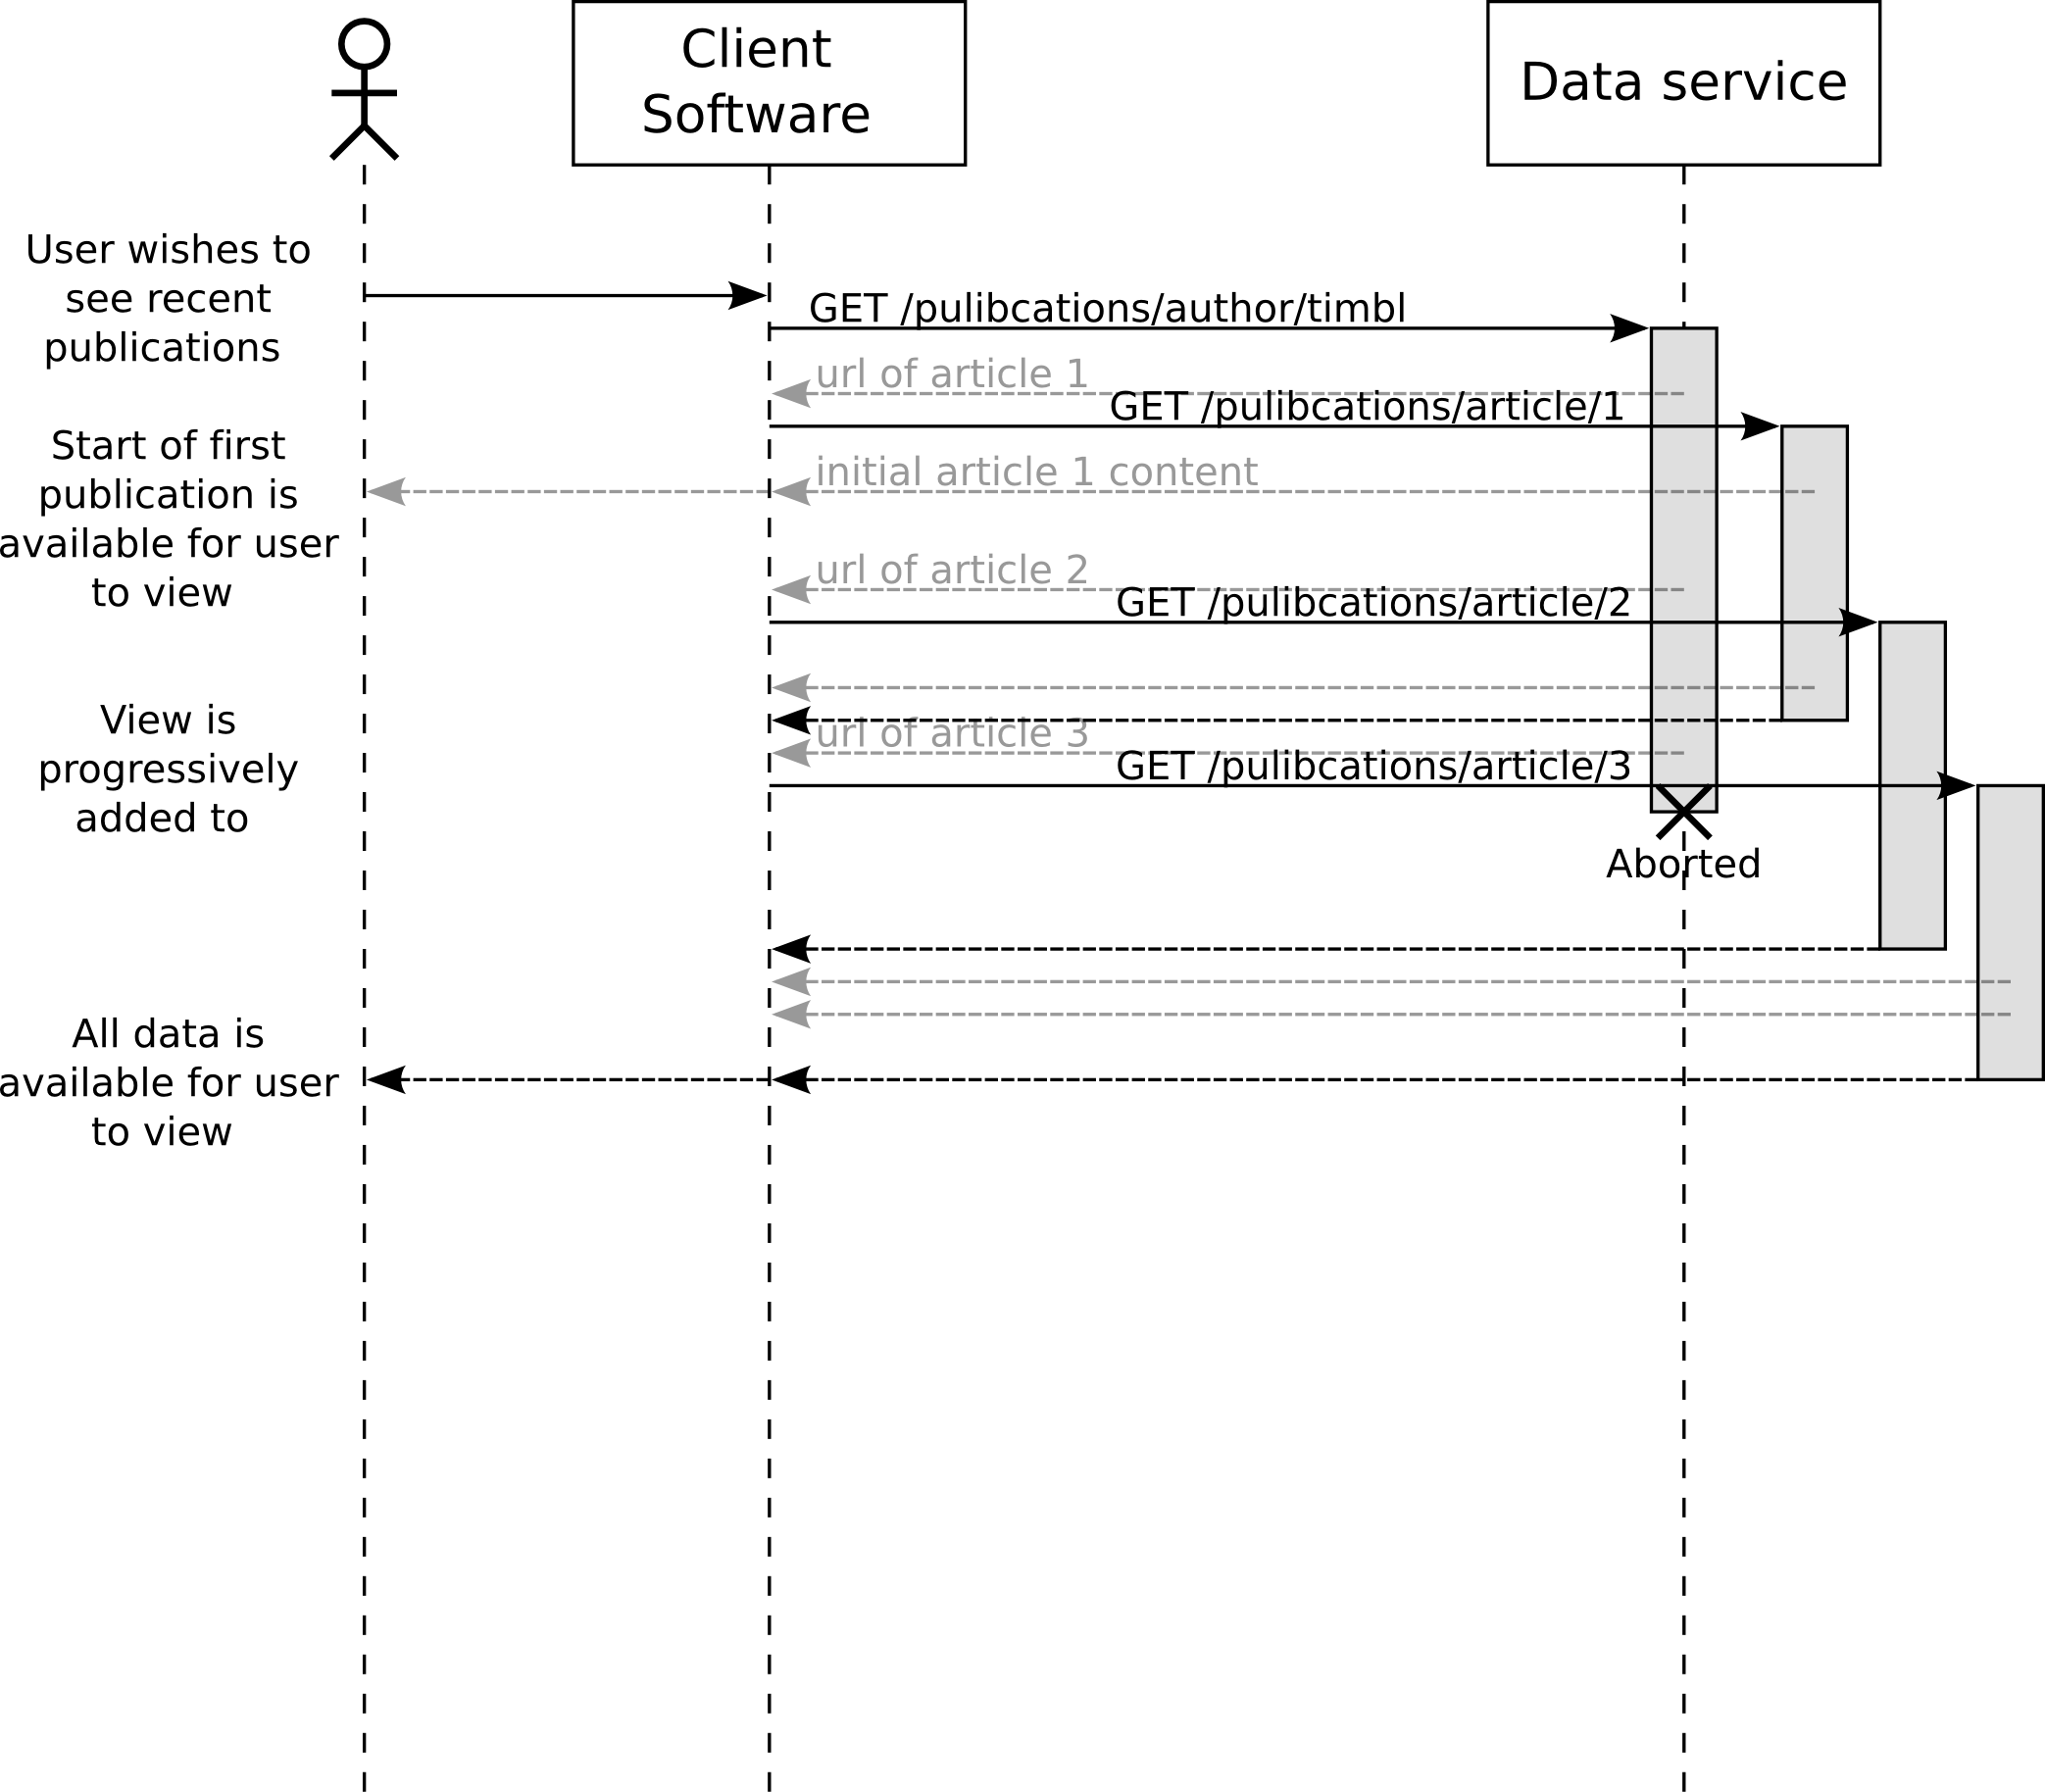
\includegraphics{images/rest_timeline_2.png}
\caption{\textbf{Revised aggregation sequence for a client capable of
progressively interpreting the resources.} Because arrows in UML
sequence diagrams draw returned values as a one-off happening rather
than a continuous process, I have introduced a lighter arrow notation
representing fragments of an incremental response. Each request for an
individual publication is made as soon as the its URL can be extracted
from the publications list and once all required data has been read from
the original response it is aborted rather than continue to download
unnecessary data. \label{rest_timeline_2}}
\end{figure}

Figures \ref{rest_timeline_1} and \ref{rest_timeline_2} comparatively
illustrate how a progressive client may, without adjustments to the
server, be used to produce an aggregated resource sooner. This results
in a moderate improvement in the time taken to show the complete
aggregation but a dramatic improvement in the time to show the first
content. The ability to present the first content as early as possible
is a desirable trait for system usability because it allows the user to
start reading earlier and a progressively rendered display in itself
increases the human perception of speed (Geelhoed et al. 1995). Note
also how the cadence of requests is more steady in Figure
\ref{rest_timeline_2} with four connections opened at roughly equal
intervals rather than a single request followed by a rapid burst of
three. Both clients and servers routinely limit the number of
simultaneous connections per peer so avoiding bursts of requests is
further to our advantage. \hyperref[appendix_http_limits]{Appendix i}
lists some actual limits.

Nodes in an n-tier architecture defy categorisation as `client' or
`server' in a way which is appropriate from all frames of reference. A
node might be labeled as the `server' from the layer below and `client'
from the layer above. Although the ``client software'' labels in the
figures above hint at something running directly on a user's own device,
the same benefits apply if this layer is running remotely. If this layer
were generating a web page on the server-side to be displayed by the
client's browser, the perceptual speed improvements apply because of
http chunked encoding (Stefanov 2009). If this layer were a remote
aggregation service, starting to write out the aggregated response early
provides much the same benefits so long as the client is also able to
interpret it progressively and, even if it were not, the overall
delivery remains faster.

\subsection{Stepping outside the big-small tradeoff}

Where a domain model contains data in a series with continuous ranges
requestable via REST, I have often noticed a tradeoff in the client's
design with regards to how much should be requested in each call.
Because at any time it shows only a small window into a much larger
model, the social networking site Twitter might be a good example. The
Twitter interface designers adopted a popular interface pattern,
Infinite Scrolling (Ahuvia 2013). Starting from an initial page showing
some finite number of tweets, once the user scrolls and reaches the end
of the list the next batch is automatically requested. When loaded, this
new batch is converted to HTML and added to the bottom of the page.
Applied repeatedly the illusion of an infinitely long page in
maintained, albeit punctuated with pauses whenever new content is
loaded. For the programmers working on this presentation layer there is
a tradeoff between sporadically requesting many tweets, yielding long,
infrequent delays and frequently requesting a little, giving an
interface which stutters momentarily but often.

I propose that progressive loading could render this tradeoff
unnecessary by simultaneously delivering the best of both strategies. In
the Twitter example this could be achieved by making large requests but
instead of deferring all rendering until the request completes, add the
individual tweets to the page as they are incrementally parsed out of
the ongoing response. With a streaming transport, the time taken to
receive the first tweet should not vary depending on the total number
that are also being sent so there is no relationship between the size of
the request made and the time taken to first update the interface.

\subsection{Staying fast on a fallible network}

REST operates over networks whose reliability varies widely. On
unreliable networks connections are abruptly dropped and in my opinion
existing http clients handle unexpected terminations suboptimally.
Consider the everyday situation of a person using a smartphone browser
to check their email. Mobile data coverage is often weak outside of
major cities (Gill 2013) so while travelling the signal will be lost and
reestablished many times. The web developer's standard AJAX toolkit is
structured in a way that encourages early terminated connections to be
considered as wholly unsuccessful rather than as partially successful.
For example, the popular AJAX library jQuery automatically parses JSON
or XML responses before passing back to the application but given an
early disconnection there is no attempt to hand over the partial
response. To the programmer who knows where to look the partial
responses are extractable as raw text but handling them involves writing
a special case and is difficult because standard parsers are not
amenable to incomplete markup. Because of this difficulty I can only
find examples of partial messages being dropped without inspection. For
the user checking her email, even if 90\% of her inbox had been
retrieved before her phone signal was lost, the web application will
behave as if it received none and show her nothing. Later, when the
network is available again the inbox will be downloaded from scratch,
including the 90\% which previously delivered. I see much potential for
improvement here.

I propose moving away from this polarised view of
successful/unsuccessful requests to one in which identifiable parts of a
message are recognised as interesting in themselves, regardless of what
follows, and these parts are handed back to the application as streaming
occurs. This follows naturally from a conceptualisation of the http
response as a progressive stream of many small parts; as each part
arrives it should be possible to use it without knowing if the next will
be delivered successfully. Should an early disconnection occur, the
content delivered up to that point will have already been handled so no
special case is required to salvage it. In most cases the only recovery
necessary will be to make a new request for just the part that was
missed. This approach is not incompatible with a problem domain where
the usefulness of an earlier part is dependent on the correct delivery
of the whole providing optimistic locking is used. In this case earlier
parts may be used immediately but their effect rolled back should a
notification of failure be received.

\subsection{Agile methodologies, frequent deployments, and compatibility
today with versions tomorrow}

In most respects a SOA architecture fits well with the fast release
cycle encouraged by Agile methodologies. Because in SOA we may consider
that all data is local rather than global and that the components are
loosely coupled and autonomous, frequent releases of any particular
sub-system shouldn't pose a problem to the correct operation of the
whole. In allowing a design to emerge organically it should be possible
for the structure of resource formats to be realised slowly and
iteratively while a greater understanding of the problem is gained.
Unfortunately in practice the ability to change is hampered by tools
which encourage programming against rigidly specified formats. If a
program is allowed to be tightly coupled to a data format it will resist
changes in the programs which produce data to that format. Working in
enterprise I have often seen the release of dozens of components
cancelled because of a single unit that failed to meet acceptance
criteria. By insisting on exact data formats, subsystems become tightly
coupled and the perfect environment is created for contagion whereby the
updating of any single unit may only be done as part of the updating of
the whole.

An effective response to this problem would be to integrate into a REST
clients the ability to use a response whilst being only loosely coupled
to the \emph{shape} of the message.

\subsection{Deliverables}

To avoid feature creep I am paring down the software deliverables to the
smallest work which can we said to realise my thesis, the guiding
principle being that it is preferable to produce a little well than more
badly. Amongst commentators on start-up companies this is known as a
\emph{zoom-in pivot} (Reis 2011 p172) and the work it produces should be
the \emph{Minimum Viable Product} or MVP (Reis 2011 p106-110). With a
focus on quality I could not deliver a full stack so I am obliged to
implement only solutions which interoperate with existing deployments.
This is advantageous; to somebody looking to improve their system small
enhancements are more inviting than wholesale change.

To reify the vision above, a streaming client is the MVP. Because all
network transmissions may be viewed though a streaming lens an
explicitly streaming server is not required. Additionally, whilst http
servers capable of streaming are quite common even if they are not
always programmed as such, I have been unable to find any example of a
streaming-receptive REST client.

\subsection{Criteria for success}

In evaluating this project, we may say it has been a success if
non-trivial improvements in speed can be made without a corresponding
increase in the difficulty of programming the client. This improvement
may be in terms of the absolute total time required to complete a
representative task or in a user's perception of the speed in completing
the task. Because applications in the target domain are much more
io-bound than CPU-bound, optimisation in terms of the execution time of
a algorithms will be de-emphasised unless especially egregious. The
measuring of speed will include a consideration of performance
degradation due to connections which are terminated early.

Additionally, I shall be considering how the semantics of a message are
expanded as a system's design emerges and commenting on the value of
loose coupling between data formats and the programs which act on them
in avoiding disruption given unanticipated format changes.

\section{Background}

\begin{figure}[htbp]
\centering
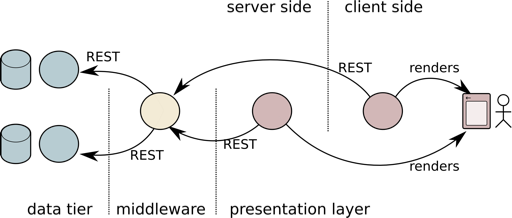
\includegraphics{images/architecture.png}
\caption{\textbf{Labelling nodes in an n-tier architecture} Regardless
of where a node is located, REST may be used as the means of
communication. By focusing on REST clients, nodes in the middleware and
presentation layer fall in our scope. Although network topology is often
split about client and server side, for our purposes categorisation as
tiers is a more meaningful distinction. According to this split the
client-side presentation layer and server-side presentation layer serve
the same purpose, generating mark-up based on aggregated data created in
the middle tier}
\end{figure}

\subsection{The web as an application platform}

Application design, particularly regarding the presentation layer, has
charted an undulating path pulled by competing strategies of thick and
thin clients. Having been taken up as the platform for all but the most
specialised applications, the web continues in this fashion by resisting
easy categorisation as either mode. Today it is agreed that program
architecture should separate presentation from operational logic but
there is no firm consensus on where each concern should be exercised.
While it feels that Javascript is becoming requisite to even display a
page, there are also actions in the opposite direction, for example in
2012 twitter moved much of their rendering back to the server-side
reducing load times to one fifth of their previous design, commenting
``The future is coming and it looks just like the past'' (Lea 2012).
This model generated server-side short pages that load quick and are
ready to be displayed but also sent the Javascript which would allow the
display to be updated without another full server load. One weakness of
this model is that the same presentational logic requires two
expressions.

Like most interactive programming, client-side scripts usually suffer
greater delays waiting for io than because javascript execution times
present a bottleneck. Because Javascript is used for user interfaces,
frame-rates are important. Single threaded so js holds up rendering.
Important to return control to the browser quickly. However, once
execution of each js frame of execution is no more than the monitor
refresh rate, further optimisation is without practical benefit. Hence,
writing extremely optimised Javascript, especially focusing on
micro-optimisations that hurt code readability is a bit silly.

\begin{quote}
The user does something, then the app responds visually with immediacy
at 30 frames per second or more, and completes a task in a few hundred
milliseconds. As long as an app meets this user goal, it doesn't matter
how big an abstraction layer it has to go through to get to silicon.
(Mullany 2013)
\end{quote}

\subsection{Node.js}

Include? Node not just for servers. CLI tools etc.

Include? Compare to Erlang. Waiter model. Node restaurant much more
efficient use of expensive resources.

Include? No `task' class or type, tasks are nothing more than functions,
possibly having some values implicitly wrapped up in their closure.

Include? Easy to distribute software (npm etc)

It is difficult to say to what degree Node's use of Javascript is a
distraction from the system's principled design aims and to what degree
it defines the technology. Paradoxically, both may be so. Javascript has
proven itself very effective as the language to meet Node's design goals
but this suitability is not based on Javascript's association with web
browsers, although it is certainly beneficial: for the first time it is
possible to program presentation logic once which is capable of running
on either client or server. Being already familiar with Javascript, web
programmers were the first to take up Node.js first but the project
mission statement makes no reference to the web; Node's architecture is
well suited to any application domain where low-latency responses to i/o
is more of a concern than heavyweight computation. Web applications fit
well into this niche but they are far from the only domain that does so.

In most imperative languages attempts at concurrency have focused on
threaded execution, whereas Node is by design single-threaded. Threads
are an effective means to speed up parallel computation but not well
suited to concurrently running tasks which are mostly i/o dependent.
Used for io, threads consume considerable resources while spending most
of their lives waiting, occasionally punctuated with short bursts of
activity. Programming Java safely with threads which share access to
mutable objects requires great care and experience, otherwise the
programmer is liable to create race conditions. If we consider for
example a Java thread-based http aggregator; each `requester' thread
waits for seconds and then processes for milliseconds. The ratio of
waiting to processing is so high that any gains achieved through actual
concurrent execution of the active phase is pyrrhic. Following Node's
lead, even traditionally thread-based environments such as Java are
starting to embrace asynchronous, single-threaded servers with projects
such as Netty.

Node manages concurrency by managing an event loop of queued tasks and
expects each task never to block. Non-blocking calls are used for all io
and are callback based. Unlike Erlang, Node does not swap tasks out
preemptively, it always waits for tasks to complete. This means that
each task must complete quickly; while this might at first seem like an
onerous requirement to put on the programmer, in practice the
asynchronous nature of the toolkit makes following this requirement more
natural than not. Indeed, other than accidental non-terminating loops or
heavy number-crunching, the lack of any blocking io whatsoever makes it
rather difficult to write a node program whose tasks do not exit
quickly. This programming model of callback-based, asynchronous,
non-blocking io with an event loop is already the model followed inside
web browsers, which although multi-threaded in some regards, present a
single-threaded virtual machine in terms of Javascript execution.

A programmer working with Node's single-thread is able to switch
contexts quickly to achieve a very efficient kind of concurrency because
of Javascript's support for closures. Because of closures, under Node
the responsibility to explicitly store state between making an
asynchronous call and receiving the callback is removed from the
programmer. Closures require no new syntax, the implicit storage of this
data feels so natural and inevitable that looking at the typical program
it is often not obvious that the responsibility exists at all.

\begin{Shaded}
\begin{Highlighting}[]

\CommentTok{// Rather than blocking, this function relies on non-blocking io and}
\CommentTok{// schedules three tasks, each of which exit quickly, allowing this}
\CommentTok{// node instance to continue with other tasks in between. }
\CommentTok{// However sophisticated and performant this style of programming, }
\CommentTok{// to the developer it is barely more difficult than if a blocking io}
\CommentTok{// model were followed. }

\KeywordTok{function} \FunctionTok{makeRequest}\NormalTok{( host, path ) \{}

   \KeywordTok{var} \NormalTok{options = \{ }\DataTypeTok{host}\NormalTok{: host, }\DataTypeTok{path}\NormalTok{: path \};}
   
   \OtherTok{http}\NormalTok{.}\FunctionTok{get}\NormalTok{(options, }\KeywordTok{function}\NormalTok{(response)\{}
      
      \CommentTok{// This function will be called when the response starts. The callback}
      \CommentTok{// having started listening to the response object will quickly exit}
      \CommentTok{// as Node tasks are want to do. Because of closures we are able to}
      \CommentTok{// access the path variable declared in a containing scope, even after}
      \CommentTok{// the containing scope has exited.      }
      \OtherTok{console}\NormalTok{.}\FunctionTok{log}\NormalTok{(}\StringTok{"The response has started for "} \NormalTok{+ path);}
   
      \OtherTok{response}\NormalTok{.}\FunctionTok{on}\NormalTok{(}\StringTok{'data'}\NormalTok{, }\KeywordTok{function}\NormalTok{(chunk) \{}
      
         \CommentTok{// This function is called each time some data is received from the }
         \CommentTok{// http request}
         
         \OtherTok{console}\NormalTok{.}\FunctionTok{log}\NormalTok{(}\StringTok{'Got some response '} \NormalTok{+ chunk);}
       
      \NormalTok{\});}
   \NormalTok{\}).}\FunctionTok{on}\NormalTok{(}\StringTok{"error"}\NormalTok{, }\KeywordTok{function}\NormalTok{(e)\{}
   
      \OtherTok{console}\NormalTok{.}\FunctionTok{log}\NormalTok{(}\StringTok{"Got error: "} \NormalTok{+ }\OtherTok{e}\NormalTok{.}\FunctionTok{message}\NormalTok{);}
   \NormalTok{\});}
   
   \OtherTok{console}\NormalTok{.}\FunctionTok{log}\NormalTok{(}\StringTok{"Request has been made"}\NormalTok{);}
\NormalTok{\}}
\end{Highlighting}
\end{Shaded}

\subsection{Streams in Node}

\begin{quote}
Streams in node are one of the rare occasions when doing something the
fast way is actually easier. SO USE THEM. not since bash has streaming
been introduced into a high level language as nicely as it is in node."
\href{https://gist.github.com/2401787}{high level node style guide}
\end{quote}

Bash streams a powerful abstraction easily programmed for linear
streaming. Node more powerful, allows a powerful streaming abstraction
which is no more complex to program than a javascript webapp front end.
Essentially a lower-level (and therefore more powerful) interface to
streaming such as unix sockets or tcp connections.

\begin{quote}
Node Stream API, which is the core I/O abstraction in Node.js (which is
a tool for I/O) is essentially an abstract in/out interface that can
handle any protocol/stream that also happens to be written in
JavaScript.
{[}\url{http://maxogden.com/a-proposal-for-streaming-xhr.html}{]}
\end{quote}

Streams in node are a variant of the observer pattern and fit into a
wider Node event model. Streams emit `readable' events when they have
some data to be read and `end' events when they are finished. Apart from
error handling, so far as reading is concerned, that is the extent of
the API.

\subsection{Web browsers hosting REST clients}

Http is essentially a thinly-wrapped text response around some usually
text-based (but sometimes binary) data. It may give the length of the
content as a header, but is not obliged to. It supports an explicitly
chunked mode, but even the non-chunked mode may be considered as a
stream. For example, a program generating web pages on the server side
might choose to use chunking so that the browser is better able to
choose when to re-render during the progressive display of a page
(Stefanov 2009) but this is optional and without these hints progressive
rendering will still take place.

The requesting of http from Javascript, commonly termed AJAX, was so
significant a technique in establishing the modern web application
architecture that it is often taken as being a synonym for
Javascript-heavy web pages. Although an acronym for Asynchronous
Javascript and XML, for data services designed with delivery to
client-side web applications in mind JSON is almost exclusively
preferred to XML and the term is used without regard for the data format
of the response (the unpronounceable \emph{AJAJ} never took off). During
the `browser war' years adding non-standard features was a common form
of competition between authors; following this pattern Internet Explorer
originally made AJAX possible by exposing Microsoft's Active X \emph{Xml
Http Request}, or XHR, object to Javascript programmers. This was widely
copied as functional equivalents were added to all major browsers and
the technique was eventually formalised by the W3C(van Kesteren and
Jackson 2006). What followed was a period of stagnation for web
browsers. HTML4 reached W3C Recommendation status in 2001 but having
subsequently found several evolutionary dead ends such as XHTML, the
developer community would see no major updates until HTML5 started to
gather pace some ten years later. In this context the web continued to
rapidly mature as an application platform and AJAX programming
inevitably overtook the original XHR specification, browser vendors
again adding their own proprietary extensions to compensate.

Given this backdrop of non-standard extensions and lagging
standardisation, abstraction layers predictably rose in popularity.
Despite a reputation Javascript being poorly standardised, as a language
it is very consistently implemented. More accurately we should say that
the libraries provided by the environment lack compatibility. Given an
abstraction layer to gloss over considerable differences cross-browser
webapp developers found little difficulty in targeting multiple
platforms. The various abstraction competed on developer ergonomics with
the popular jQuery and Prototype.js promoting themselves respectively as
\emph{``do more, write less''} and \emph{``elegant APIs around the
clumsy interfaces of Ajax''}. JSON being a subset of Javascript, web
developers barely noticed their privileged position whereby the
serialisation of their data format mapped exactly onto the basic types
of their programming language. As such there was never any confusion as
to which exact object structure to de-serialise to. If this seems like a
small advantage, contrast with the plethora of confusing and
incompatible representations of JSON output presented by the various
Java JSON parsers; JSON's Object better resembles Java's Map than Object
and the confusion between JSON null, Java null, and Jackson's
NullNode\footnote{See
  \url{http://jackson.codehaus.org/1.0.1/javadoc/org/codehaus/jackson/node/NullNode.html}.}
is a common cause of errors. Endowed with certainty regarding
deserialisation, JSON parsers could be safely integrated directly into
AJAX libraries. This provided a call style while working with remote
resources so streamlined as to require hardly any additional effort.

\begin{Shaded}
\begin{Highlighting}[]
\OtherTok{jQuery}\NormalTok{.}\FunctionTok{ajax}\NormalTok{(}\StringTok{'http://example.com/people.json'}\NormalTok{, }\KeywordTok{function}\NormalTok{( people ) \{}

   \CommentTok{// The parsing of the people json into a javascript object}
   \CommentTok{// feels so natural that it is easy to forget while looking }
   \CommentTok{// at the code that it happens at all. }
   
   \FunctionTok{alert}\NormalTok{(}\StringTok{'the first person is called '} \NormalTok{+ people[}\DecValTok{0}\NormalTok{].}\FunctionTok{name}\NormalTok{);}
\NormalTok{\});}
\end{Highlighting}
\end{Shaded}

Whilst simple, the above call style is built on the assumption that a
response is a one-time event and no accommodation is made for a
continuously delivered response. Meanwhile, the XHR2 standardisation
process had started and was busy observing and specifying proprietary
extensions to the original XHR1. Given an interest in streaming, the
most interesting of these is the progress event:

\begin{quote}
While the download is progressing, queue a task to fire a progress event
named progress about every 50ms or for every byte received, whichever is
least frequent. (van Kesteren 2012)
\end{quote}

Prior to this addition there had been no mechanism, at least so far as
the published specs to an XHR instance in a streaming fashion. However,
while all major browsers currently support progress events in their most
recently versions, the installed userbase of supporting browsers is
unlikely to grow fast enough that this technique may be relied upon
without a fallback for several years.

In fact, this is exactly how web browsers are implemented. However, this
progressive use of http is hardwired into the browser engines rather
than exposing an API suitable for general use and as such is treated as
something of a special case specific to web browsers and has not so far
seen a more general application. I wish to argue that a general
application of this technique is viable and offers a worthwhile
improvement over current common methods.

While until recently browsers have provided no mechanism to stream into
AJAX, almost every other instance of downloading has taken advantage of
streaming and progressive interpretation. This includes image formats,
as the progressive PNG and JPEG; markup as progressive display of html
and svg; video; and Javascript itself -- script interpretation starts
before the script is wholly fetched. Each of these progressive
considerations is implemented as a specific-purpose mechanism internal
to the browser which is not exported to Javascript and as such is not
possible to repurpose.

\subsection{Browser streaming frameworks}

As the web's remit spread to include more applications which would
previously have been native apps, to be truly `live' many applications
found the need to be able to receive real-time push events. Dozens of
streaming transports have been developed sidestepping the browser's
apparent limitations.

The earliest and most basic attempt was to poll by making many requests,
I won't consider this approach other than to say it came with all the
usually associated downsides. Despite the inadequacy of this approach,
from here the improved technique of \emph{long polling} was invented. A
client makes a request to the server side. Once the connection is open
the server waits, writing nothing until a push is required. To push the
server writes the message and closes the http connection; since the http
response is now complete the content may be handled by the Javascript
client which then immediately makes a new request, reiterating the cycle
of wait and response. This approach works well where messages are
infrequently pushed but where the frequency is high the limitation of
one http transmission per connections requires imposes a high overhead.

Observing that while browsers lack progressive ajax, progressive html
rendering is available, \emph{push tables} achieve progressive data
transfer by serialising streaming data to a HTML format. Most commonly
messages are written to a table, one row per message. On the client side
this table is hidden in an off-screen frame and the Javascript streaming
client watches the table and reacts whenever a new row is found. In many
ways an improvement over long-polling, this approach nevertheless
suffers from an unnatural data format. Whilst html is a textual format
so provides a degree of human-readability, html was not designed with
the goal of an elegent or compact transfer of asynchronous data.
Contrasted with a SOA ideal of \emph{`plumbing on the outside'}, peeking
inside the system is difficult whilst bloated and confusing formats are
tasked with conveying meaning.

Both long polling and push tables are better throught of as a means to
circumvent restrictions than indigene technology. A purose-built stack,
\emph{Websockets} is poised to take over, building a standardised duplex
transport and API on top of http's chunked mode. While the newest
browsers support websockets, most of the wild use base does not. Nor do
older browsers provide a fine-grained enough interface into http in
order to allow a Javascript implementation. In practice, real-world
streaming libraries such as socket.io {[}CITE{]} are capable of several
streaming techniques and can select the best for a given context. To the
programmer debugging an application the assortment of transports only
enhances the black-box mentality with regards to the underlying
transports.

Whilst there is some overlap, each of the approaches above addresses a
problem only tangentially related to this project's aims. Firstly,
requiring a server that can write to an esoteric format feels quite
anti-REST, especially given that the server is sending in a format which
requires a specific, known, specialised client rather than a generic
tool. In REST I have always valued how prominently the plumbing of a
system is visible, so that to sample a resource all that is required is
to type a URL and be presented with it in a human-comprehensible format.

Secondly, as adaptations to the context in which they were created,
these frameworks realise a view of network usage in which downloading
and streaming are dichotomously split, whereas I aim to realise a schema
without dichotomy in which \emph{streaming is adapted as the most
effective means of downloading}. In existing common practice a wholly
distinct mechanism is provided vs for data which is ongoing vs data
which is finite. For example, the display of real-time stock data might
start by AJAXing in historical and then separately use a websocket to
maintain up-to-the-second updates. This requires the server to support
two distinct modes. However, I see no reason why a single transport
could not be used for both. Such a server might start answering a
request by write historic events from a database, then switch to writing
out live data in the same format in response to messages from a MOM. By
closing the dichotomy we would have the advantage that a single
implementation is able to handle all cases.

It shouldn't be a surprise that a dichotomous implementation of
streaming, where a streaming transport is used only for live events is
incompatible with http caching. If an event is streamed when it is new,
but then when it is old made available for download, http caching
between the two requests is impossible. However, where a single mode is
used for both live and historic events the transport is wholly
compatible with http caching.

If we take streaming as a technique to achieve efficient downloading,
not only for the transfer of forever-ongoing data, none of these
approaches are particularly satisfactory.

\subsection{Json and XML}

\emph{later mention JSON `nodes'/`paths' a lot. Good place to intro
here}

Although AJAX started as a means to transfer XML, today JSON ``The
fat-free alternative to XML(Douglas 2009)'' is the more popular
serialisation format. The goals of XML were to simplify SGML to the
point that a graduate student would be able to implement a parser in a
week {[}@javaxml p ???{]}. For the student tackling JSON a few hours
with a parser generator should surfice, being expressable in 15 CFGs.
Indeed, because JSON is a strict subset of Javascript, in many cases the
Javascript programmer requires no parser at all. Unimpeeded by SGML's
roots as a document format, JSON provides a much more direct analogue to
the metamodel of a canonical modern programming language with entities
such as \emph{string}, \emph{number}, \emph{object} and \emph{array}. By
closely mirroring a programmer's metamodel, visualising a mapping
between a domain model and it's serialised objects becomes trivial.

\begin{Shaded}
\begin{Highlighting}[]
\NormalTok{\{}
   \DataTypeTok{people}\NormalTok{: [}
      \NormalTok{\{}\DataTypeTok{name}\NormalTok{: }\StringTok{'John'}\NormalTok{, }\DataTypeTok{town}\NormalTok{:}\StringTok{'Oxford'}\NormalTok{\},}
      \NormalTok{\{}\DataTypeTok{name}\NormalTok{: }\StringTok{'Jack'}\NormalTok{, }\DataTypeTok{town}\NormalTok{:}\StringTok{'Bristol'}\NormalTok{\}}
   \NormalTok{]}
\NormalTok{\}}
\end{Highlighting}
\end{Shaded}

This close resemblance to the model of the programming in some cases
causes fast-changing formats.

Like XML attributes, as a serialised text format, JSON objects have an
order but are almost always parsed to and from orderless maps meaning
that the order of the keys/value pairings as seen in the stream usually
follows no defined order. No rule in the format would forbid
representing of an ordered map in an ordered way but most tools on
receiving such a message would ignore the ordering.

(MINE SOA assignment). Also the diagram.

\subsection{Parsing: SAX and Dom}

In the XML world two standard parser models exist, SAX and DOM, with DOM
far the more popular. DOM performs a parse as a single evaluation, on
the request of the programmer, returning an object model representing
the whole of the document. At this level of abstraction the details of
the markup are only distant concern. Conversely, SAX parsers are
probably better considered as tokenisers, providing a very low-level
event driven interface in line with the Observer pattern to notify the
programmer of syntax as it is seen. Each element's opening and closing
tag is noted

This presents poor developer ergonomics by requiring that the programmer
implement the recording of state with regard to the nodes that they have
seen. For programmers using SAX, a conversion to their domain objects is
usually implemented imperatively. This programming tends to be difficult
to read and programmed once per usage rather than assembled as the
combination of reusable parts. For this reason SAX is usually reserved
for fringe cases where messages are very large or memory unusually
scarce.

DOM isn't just a parser, it is also a cross-language defined interface
for manipulating the XML in real time, for example to change the
contents of a web page in order to provide some interactivity. In JSON
world, DOM-style parser not referring to the DOM spec, or what browser
makers would mean. Rather, borrowing from the XML world to mean a parser
which requires the whole file to be loaded.

Suppose we want to extract the name of the first person. Given a DOM
parser this is very easy:

\begin{Shaded}
\begin{Highlighting}[]
\KeywordTok{function} \FunctionTok{nameOfFirstPerson}\NormalTok{( myJsonString ) \{}

   \CommentTok{// Extracting an interesting part from JSON-serialised data is}
   \CommentTok{// relatively easy given a DOM-style parser. Unfortunately this}
   \CommentTok{// forbids any kind of progressive consideration of the data.}
   \CommentTok{// All recent browsers provide a JSON parser as standard. }

   \KeywordTok{var} \NormalTok{document = }\OtherTok{JSON}\NormalTok{.}\FunctionTok{parse}\NormalTok{( myJsonString );}
   \KeywordTok{return} \OtherTok{document}\NormalTok{.}\FunctionTok{people}\NormalTok{[}\DecValTok{0}\NormalTok{].}\FunctionTok{name}\NormalTok{; }\CommentTok{// that was easy!}
\NormalTok{\}}
\end{Highlighting}
\end{Shaded}

Contrast with the programming below which uses the clarinet JSON SAX
parser. To prove that I'm not exaggerating the case, see published
usages at {[}Clarinet demos{]}.

\pagebreak

\begin{Shaded}
\begin{Highlighting}[]
\KeywordTok{function} \FunctionTok{nameOfFirstPerson}\NormalTok{( myJsonString, callbackFunction )\{}

   \CommentTok{// The equivalent logic, expressed in the most natural way}
   \CommentTok{// fora s JSON SAX parser is longer and much more }
   \CommentTok{// difficult to read. The developer pays a high price for }
   \CommentTok{// progressive parsing. }

   \KeywordTok{var} \NormalTok{clarinet = }\OtherTok{clarinet}\NormalTok{.}\FunctionTok{parser}\NormalTok{(),}
   
       \CommentTok{// with a SAX parser it is the developer's responsibility }
       \CommentTok{// to track where in the document the cursor currently is,}
       \CommentTok{// requiring several variables to maintain.        }
       \NormalTok{inPeopleArray = }\KeywordTok{false}\NormalTok{,   }
       \NormalTok{inPersonObject = }\KeywordTok{false}\NormalTok{,}
       \NormalTok{inNameAttribute = }\KeywordTok{false}\NormalTok{,}
       \NormalTok{found = }\KeywordTok{false}\NormalTok{;}
   
   \OtherTok{clarinet}\NormalTok{.}\FunctionTok{onopenarray} \NormalTok{= }\KeywordTok{function}\NormalTok{()\{}
      \CommentTok{// for brevity we'll cheat by assuming there is only one}
      \CommentTok{// array in the document. In practice this would be overly}
      \CommentTok{// brittle.}
      
      \NormalTok{inPeopleArray = }\KeywordTok{true}\NormalTok{; }
   \NormalTok{\};}
   
   \OtherTok{clarinet}\NormalTok{.}\FunctionTok{onclosearray} \NormalTok{= }\KeywordTok{function}\NormalTok{()\{}
      \NormalTok{inPeopleArray = }\KeywordTok{false}\NormalTok{;}
   \NormalTok{\};   }
   
   \OtherTok{clarinet}\NormalTok{.}\FunctionTok{onopenobject} \NormalTok{= }\KeywordTok{function}\NormalTok{()\{}
      \NormalTok{inPersonObject = inPeopleArray; }
   \NormalTok{\};}
   
   \OtherTok{clarinet}\NormalTok{.}\FunctionTok{oncloseobject} \NormalTok{= }\KeywordTok{function}\NormalTok{()\{}
      \NormalTok{inPersonObject = }\KeywordTok{false}\NormalTok{;}
   \NormalTok{\};   }
      
   \OtherTok{clarinet}\NormalTok{.}\FunctionTok{onkey} \NormalTok{= }\KeywordTok{function}\NormalTok{(key)\{}
      \NormalTok{inNameAttribute = ( inPeopleObject && key == }\StringTok{'name'}\NormalTok{);}
   \NormalTok{\};}

   \OtherTok{clarinet}\NormalTok{.}\FunctionTok{onvalue} \NormalTok{= }\KeywordTok{function}\NormalTok{(value)\{}
      \KeywordTok{if}\NormalTok{( !found && inNameAttribute ) \{}
         \CommentTok{// finally!}
         \FunctionTok{callbackFunction}\NormalTok{( value );}
         \NormalTok{found = }\KeywordTok{true}\NormalTok{;}
      \NormalTok{\}}
   \NormalTok{\};      }
   
   \OtherTok{clarinet}\NormalTok{.}\FunctionTok{write}\NormalTok{(myJsonString);   }
\NormalTok{\}}
\end{Highlighting}
\end{Shaded}

As we can see above, SAX's low-level semantics require a lengthy
expression and for the programmer to maintain state regarding the
position in the document -- usually recording the ancestors seen on the
descent from the root to the current node -- in order to identify the
interesting parts. This order of the code is also quite unintuitive;
generally event handlers will cover multiple unrelated concerns and each
concern will span multiple event handlers. This lends to programming in
which separate concerns are not separately expressed in the code.

\subsection{Common patterns when connecting to REST services}

Marshaling provides two-way mapping between a domain model and a
serialisation as JSON or XML, either completely automatically or based
on a declarative specification. To handle a fetched rest response it is
common to automatically demarshal it so that the application may make
use of the response from inside its own model, no differently from
objects assembled in any other way. From the perspective of the
programmer it is as if the domain objects themselves had been fetched.
Another common design pattern, intended to give a degree of isolation
between concerns, is to demarshal automatically only so far as Data
Transfer Objects (DTOs), instances of classes which implement no logic
other than storage, and from there programmatically instantiate the
domain model objects. Going one step further, for JSON resources sent to
loosely-typed languages with a native representation of objects as
generic key-value pairs such as Javascript or Clojure, the marshaling
step is often skipped: the output from the parser so closely resembles
the language's built-in types that it is simplest to use it directly.
Depending on the programming style adopted we might say that the JSON
parser's output \emph{is} the DTO and create domain model objects based
on it, or that no further instantiation is necessary.

\begin{figure}[htbp]
\centering

\includegraphics{images/placeholder.png}
\caption{\emph{Degrees of automatic marshaling}. From marshaling
directly to domain objects, DTOs, using parser output as a DTO, or using
objects directly. Distinguish work done by library vs application
programmer's domain}
\end{figure}

Ultimately the degree of marshaling that is used changes only the level
of abstraction of the resource that the REST client library hands over
to the application developer. Regardless of the exact form of the
response model, the developer will usually programmatically extract one
or more parts from it via calls in the programming language itself. For
example, on receiving a resource de-marshaled to domain objects, a Java
developer will inspect it by calling a series of getters in order to
narrow down to the interesting parts. This is not to say that the whole
of the message might not in some way be interesting, only that by using
it certain parts will need to be identified as distinct areas of
concern.

\begin{Shaded}
\begin{Highlighting}[]
\CommentTok{// An example programmatic approach to a domain model interrogation }
\CommentTok{// under Java; upon receiving a list of people, each person's name}
\CommentTok{// is added to a database. The methods used to drill down to the}
\CommentTok{// pertinent components of the response are all getters: getPeople, }
\CommentTok{// getGivenName, and getSurname. }
\DataTypeTok{void} \FunctionTok{handleResponse}\NormalTok{( RestResponse response ) \{}

   \KeywordTok{for}\NormalTok{( Person p : response.}\FunctionTok{getPeople}\NormalTok{() ) \{}
      \FunctionTok{addNameToDb}\NormalTok{( p.}\FunctionTok{getGivenName}\NormalTok{(), p.}\FunctionTok{getSurname}\NormalTok{() );}
   \NormalTok{\}   }
\NormalTok{\}}
\end{Highlighting}
\end{Shaded}

\begin{Shaded}
\begin{Highlighting}[]
\CommentTok{// Although in this Javascript example the objects passed to the handler }
\CommentTok{// remain in the form given by the JSON parser, containing no domain-specific}
\CommentTok{// getters, the programming represents a different expression of the same }
\CommentTok{// basic process.}
\KeywordTok{function} \FunctionTok{handleResponse}\NormalTok{( response )\{}

   \OtherTok{response}\NormalTok{.}\OtherTok{people}\NormalTok{.}\FunctionTok{forEach}\NormalTok{( }\KeywordTok{function}\NormalTok{( person )\{}
      \FunctionTok{addNameToDb}\NormalTok{( }\OtherTok{p}\NormalTok{.}\FunctionTok{givenName}\NormalTok{, }\OtherTok{p}\NormalTok{.}\FunctionTok{surname} \NormalTok{);}
   \NormalTok{\});}
\NormalTok{\}}
\end{Highlighting}
\end{Shaded}

Because it is applied directly to the metamodel of the language{[}\^{}
It could be argued that getters aren't a part of the metamodel of Java
itself, but they form such a common pattern that it is a part {]}, this
extraction has become such a natural component of a workflow that it
maye be used while thinking of it as wholly unremarkable. In the
examples above we are interacting with the model in the way that the
language makes the most easy to conceptualise. However se should
consider that, however subtly embedded, the technique is an invented
construct and only one of the possible formulations which might have
been drawn.

One weakness of this inspection model is that, once much code is written
to interrogate models in this way, the interface of the model becomes
increasingly expensive to change as the code making the inspections
becomes more tightly coupled with the thing that it is inspecting.
Taking the above example, if the model were later refactored such that
the concepts of firstName and surName were pulled from the Person class
into an extracted Name class, because the inspection relies on a
sequence of calls made directly into domain objects, the code making the
query would also have to change. Whilst following the object oriented
principle of encapsulation of data, such that the caller does not have
to concern themselves with the data structures hidden behind the getter,
there is no such abstraction for when the structure itself changes.
Given an Agile environment where the shape of data is refactored
regularly, this would be a problem when programming against any kind of
resource; for example, if change of objects formats propagates knock-on
changes where ever the object is used it is very difficult to commit
small diffs to the VCS which make incremental changes to a tightly
focused area of the system. A method of programming which truly embraced
extreme programming would allow constant change without disparate,
barely related parts having to be modified in parallel when structural
refactoring occurs. The coupling is all the more acute where the format
of the item being inspected is defined by an independently maintained
service.

\emph{contagion problem}

Extraneous changes dilute the changelog, making it less easily defined
by code changes which are intrinsically linked to the actual change in
the logic being expressed by the program, and therefore to the thinking
behind the change and the reason for the change.

\subsection{JsonPath and XPath}

Both the above difficulty in identifying the interesting parts of a
message whilst using a streaming parser and the problem with tight
coupling of programmatic drilling down to REST formats leads me to
search for areas where this problem has already been solved.

In the domain of markup languages there are associated query languages
such as XPATH whose coupling is loose enough that their expressions may
continue to function after the exact shape of a message is refactored.
While observing this is nothing more radical than using the query
languages in more-or-less they were intended, their employment is not
the most natural coming from a programming context in which the
application developer's responsibilities usually start where the
demarshaler's end. Consider the following XML:

\begin{Shaded}
\begin{Highlighting}[]
\KeywordTok{<people>}
   \KeywordTok{<person>}
      \KeywordTok{<givenName>}\NormalTok{...}\KeywordTok{</givenName>}   
      \KeywordTok{<familyName>}\NormalTok{Bond}\KeywordTok{</familyName>}
   \KeywordTok{</person>}
\KeywordTok{</people>}
\end{Highlighting}
\end{Shaded}

The XPath //person{[}0{]}//surname//text() would continue to identify
the correct part of the resource without being updated after the xml
analogue of the above Java Name refactor:

\begin{Shaded}
\begin{Highlighting}[]
\KeywordTok{<people>}
   \KeywordTok{<person>}
      \KeywordTok{<name>}
         \KeywordTok{<givenName>}\NormalTok{...}\KeywordTok{</givenName>}
         \KeywordTok{<familyName>}\NormalTok{Bond}\KeywordTok{</familyName>}
      \KeywordTok{</name>}
   \KeywordTok{</person>}
\KeywordTok{</people>}
\end{Highlighting}
\end{Shaded}

Luckily in JSON there exists already an attempt at an equivalent named
Jsonpath. JsonPath closely resembles the javascript code which would
select the same nodes. Not a real spec.

\begin{Shaded}
\begin{Highlighting}[]

\CommentTok{// an in-memory person with a multi-line address:}
\KeywordTok{let} \NormalTok{person = \{}
   \DataTypeTok{name}\NormalTok{: \{}\DataTypeTok{givenName}\NormalTok{:}\StringTok{''}\NormalTok{, }\DataTypeTok{familyName}\NormalTok{:}\StringTok{''}\NormalTok{\},}
   \DataTypeTok{address}\NormalTok{: [}
      \StringTok{"line1"}\NormalTok{,}
      \StringTok{"line2"}\NormalTok{,}
      \StringTok{"line3"}
   \NormalTok{]}
\NormalTok{\}}


\CommentTok{// in javascript we can get line two of the address as such:}
\KeywordTok{let} \NormalTok{address = }\OtherTok{person}\NormalTok{.}\FunctionTok{address}\NormalTok{[}\DecValTok{2}\NormalTok{]}

\CommentTok{// the equivalent jsonpath expression is identical:}
\KeywordTok{let} \NormalTok{jsonPath = }\StringTok{"person.address[2]"}

\CommentTok{// although jsonpath also allows ancestor relationships which are not}
\CommentTok{// expressible quite so neatly as basic Javascript:}
\KeywordTok{let} \NormalTok{jsonPath2 = }\StringTok{"person..given"}
\end{Highlighting}
\end{Shaded}

Xpath is able to express identifiers which often survive refactoring
because XML represents a tree, hence we can consider relationships
between entities to be that of contains/contained in (also siblings?).
In application of XML, in the languages that we build on top of XML, it
is very natural to consider all elements to belong to their ancestors.
Examples are myriad, for example consider a word count in a book written
in DOCBook format - it should be calculable without knowing if the book
is split into chapters or not since this is a concept internal to the
organisation of the book itself nd not something that a querier is
likely to find interesting - if this must be considered the structure
acts as barrier to information rather than enabling the information's
delivery. Therefore, in many cases the exact location of a piece of
information is not as important as a more general location of x being in
some way under y.

This may not always hold. A slightly contrived example might be if we
were representing a model of partial knowledge:

\begin{Shaded}
\begin{Highlighting}[]
\KeywordTok{<people>}
   \KeywordTok{<person>}
      \KeywordTok{<name>}
         \KeywordTok{<isNot><surname>}\NormalTok{Bond}\KeywordTok{</surname></isNot>}
      \KeywordTok{</name>}
   \KeywordTok{</person>}
\KeywordTok{</people>}
\end{Highlighting}
\end{Shaded}

The typical use pattern of XPath or JSONPath is to search for nodes once
the whole serialisation has been parsed into a DOM-style model. JSONPath
implementation only allows for search-type usage:
\url{https://code.google.com/p/jsonpath/To} examine a whole document for
the list of nodes that match a jsonpath expression the whole of the tree
is required. But to evaluate if a single node matches an expression,
only the \emph{path of the descent from the root to that node} is
required -- the same state as a programmer usually maintains whilst
employing a SAX parser. This is possible because JSONPath does not have
a way to express the relationship with sibling nodes, only ancestors and
decedents.

One limitation of the JSONPath language is that it is not possible to
construct an `containing' expression. CSS4 allows this in a way that is
likely to become familiar to web developers over the next five years or
so.

\subsection{Testing}

\begin{figure}[htbp]
\centering

\includegraphics{images/placeholder.png}
\caption{Relationship between the main players in the JS testing
landscape. JSTD, Karma, Jasmine, NodeUnit, jasmine-node, Browsers}
\end{figure}

By the commonjs spec, test directory should be called `test'
(\url{http://wiki.commonjs.org/wiki/Packages/1.0}\#Package\_Directory\_Layout)
doesn't matter for my project since not using commonjs, but might as
well stick to the convention.

How TDD helps How can fit into methodology

\begin{itemize}
\itemsep1pt\parskip0pt\parsep0pt
\item
  JSTD
\item
  NodeUnit
\item
  Karma
\item
  Jasmine
\end{itemize}

Initially started with jstestdriver but found it difficult. Karma
started because engineers working on the Angular project in Google were
``struggling a lot with jstd'':
\url{http://www.youtube.com/watch?v=MVw8N3hTfCI} - jstd is a google
project Even Jstd's authors seems to be disowning it slightly. Describe
what was once its main mode of operation as now being for stress testing
of jstd itself only. Problems: browsers become unresponsive. Generally
unreliable, has to be restarted frequently.

JSTD, as a Java program, is difficult to start via Grunt. Also an issue
that Grunt post-dates Karma by enough that JSTD doesn't have the
attention of the Grunt community.

\section{Design and Reflection:}

Using a combination of the techniques investigated in the previous
chapter, I propose that a simple design is possible which makes REST
clients more efficient whilst being no more difficult to program.
Although simple, this model fits poorly with established vocabulary,
requiring a transport that sits \emph{somewhere between `stream' and
`download'} and a parsing strategy which \emph{takes elements from SAX
and DOM} but follows neither model.

Implementation in Javascript gives me the widest deployment options,
covering client-side browser programming, server programming, use in
command line tools, or any other usage. This context dictates a design
which is non-blocking, asynchronous and callback based. While influenced
by the language, the model of REST client proposed here is not limited
to Javascript or web usage and I intent to comment briefly also on the
applicability to other platforms. Likewise, I have also chosen to focus
on JSON although I will also be commenting on the parallel applicability
of these ideas to XML.

From DOM we may observe that as a programmer, using a resource is
simpler when a parsed entity is passed whole to a single callback,
rather than the SAX model which requires the programmer to infer the
entity from a lengthy series of callbacks. From observing SAX parsers or
progressive HTML rendering, we can say that http is more efficient if we
no not wait until we have everything before we start using the parts
that we do have. DOM parsers pass a fully parsed node to registered
callbacks, whole and ready to use, invariably at the root of the parsed
document. From the vantage of the library's user, my thesis duplicates
this convenience but removes one restriction; that the node which is
passed must be the root. Because the mark-up formats we are dealing with
are hierarchical and serialised depth-first it is possible to fully
parse any sub-tree without fully knowing the parent node. From these
observations we may program a new kind of REST client which is as
performant as SAX but as easy to program as DOM.

To follow this progressive-but-complete model, identifying the
interesting parts of a document involves turning the traditional model
for drilling down inside-out. Traditionally the programmer's callback
receives the document then inside that callback drills down to locate
the parts that they are interested in. Instead I propose taking the
drilling-down logic out from inside the callback and instead wrap the
callback in it. This means that the callback receives selected parts of
the response which the library has already drilled down to on behalf of
the programmer.

Whilst JSONPath's existing implementation is only implemented for
searching over already gathered objects, this kind of searching is just
one application for the query language. I find that this is a very
suitable declarative language to use to specify the parts of a response
that a developer would like to drill-down to given the context of a
document whose parse is in progress. JSONPath is especially applicable
because it specifies only `contained-in/contains' type relationships. On
encountering any node in a serialised JSON stream, because of the
depth-first serialisation order I will always have previously seen its
ancestors. Hence, having written a suitably flexible JSONPath expression
compiler such that it does not require a complete document, I will have
enough information to evaluate any expression against any node at the
time when it is first identified in the document. Because XML is also
written depth-first, the same logic would apply to an XPath/XML variant
of this project.

The definition of `interesting' will be generic and accommodating enough
so as to apply to any data domain and allow any granularity of interest,
from large object to individual datums. With just a few lines of
programming

\subsection{JSONPath and types}

Given its use to identify interesting parts of a document, not all of
the published JSONPath spec is useful. Parts of a document will be
considered interesting because of their type, position, or both. This
contrasts with filter-type queries such as `books costing less than X'.
Examining REST responses it is likely we will not be explicitly
searching through a full model but rather selecting from a resource
subset that the programmer requested, assembled on their behalf using
their parameters so we can expect the developer to be interested in most
of the content. In creating a new JSONPath implementation, I have chosen
to follow the published spec only loosely, thereby avoiding writing
unnecessary code. This is especially the case, as in the books example
above whereby a user of the library could easily add the filter in the
callback itself. Following the principle of writing less, better I feel
it is better to deliver only the features I am reasonably certain will
be well used but keep open the ability to add more later should it be
required.

JSON markup describes only a few basic types. On a certain level this is
also true for XML -- most nodes are of either type Elements or Text.
However, the XML metamodel provides tagnames, essentially a built-in
Element sub-typing mechanism. Floating above this distinction, a reader
abstracting over the details of the markup may forget that a node is an
Element instance and describe it as an instance of its tagname, without
considering that the tagname is a sub-type of Element. JSON comes with
no such built-in type description language. On top of JSON's largely
typeless model we often place a concept of type. Drawing parallels with
the physical world, this imposition of type is the responsibility of the
observer, rather than of the observed. A document reader has a free
choice of the taxonomy they will use to impose type on the parts of the
document, and this decision will vary depending on the purpose of the
reader. The specificity required of a taxonomy differs by the level of
involvement in a field, whereas `watch' may be a reasonable type to most
data consumers, to a horologist it is unlikely to be satisfactory
without further sub-types. In the scope of this dissertation, since
selecting on type is desirable, my JSONPath variant must be able to
distinguish types at various levels of specificity; whilst my selection
language will have no inbuilt concept of type, the aim is to support
programmers in creating their own.

\emph{integrate with above or discard, maybe move to compatibility with
future versions} Relationship between type of a node and its purpose in
the document (or, perhaps, the purpose the reader wishes to put it to).
Purpose is often obvious from a combination of URL and type so can
disregard the place in the document. This structure may be carefully
designed but ultimately a looser interpretation of the structure can be
safer.

\begin{Shaded}
\begin{Highlighting}[]
\CommentTok{<!--  XML leaves no doubt as to the labels we give to the types}
\CommentTok{      of the nodes. This is a 'person' -->}
\KeywordTok{<person}\OtherTok{  name=}\StringTok{'...'}\OtherTok{ gender=}\StringTok{"male"}
\OtherTok{         age=}\StringTok{"45"}\OtherTok{ height=}\StringTok{"175cm"}\OtherTok{ profession=}\StringTok{"architect"}\KeywordTok{>}
\KeywordTok{</person>}
\end{Highlighting}
\end{Shaded}

\begin{Shaded}
\begin{Highlighting}[]
\CommentTok{/*    JSON meanwhile provides no such concrete concept. This node's}
\CommentTok{      type might be 'thing', 'animal', 'human', 'man', 'architect',}
\CommentTok{      'artist' or any other of many overlapping impositions depending }
\CommentTok{      on what purpose the document it is read for */}
\NormalTok{\{  }\StringTok{"name"}\NormalTok{:}\StringTok{"..."}\NormalTok{, }\StringTok{"gender"}\NormalTok{:}\StringTok{"male"}\NormalTok{, }\StringTok{"age"}\NormalTok{:}\StringTok{"45"} 
   \StringTok{"height"}\NormalTok{:}\StringTok{"175cm"} \StringTok{"profession"}\NormalTok{:}\StringTok{"architect"}\NormalTok{>}
\NormalTok{\}         }
\end{Highlighting}
\end{Shaded}

In the absence of node typing beyond the categorisation as objects,
arrays and various primitive types, the key immediately mapping to the
object is often taken as a lose concept of the type of the object. Quite
fortunately, rather than because of a well considered object design,
this tends to play well with automatically marshaling of domain objects
expressed in a Java-style OO language because there is a strong tendency
for field names -- and by extension, `get' methods -- to be named after
the \emph{type} of the field, the name of the type also serving as a
rough summary of the relationship between two objects. See figure
\ref{marshallTypeFig} below.

In the below example, we impose the the type `address' because of the
parent node's field name. Other than this, these are standard arrays of
strings:

\begin{Shaded}
\begin{Highlighting}[]
\NormalTok{\{}
   \DataTypeTok{name}\NormalTok{: }\StringTok{'...'}
\NormalTok{,  }\DataTypeTok{residence}\NormalTok{: \{}
      \DataTypeTok{address}\NormalTok{: [}
         \StringTok{'...'}\NormalTok{, }\StringTok{'...'}\NormalTok{, }\StringTok{'...'}
      \NormalTok{]}
   \NormalTok{\}}
\NormalTok{,  }\DataTypeTok{employer}\NormalTok{: \{}
      \DataTypeTok{name}\NormalTok{: }\StringTok{'...'}
   \NormalTok{,  }\DataTypeTok{address }\NormalTok{:[}
         \StringTok{'...'}\NormalTok{, }\StringTok{'...'}\NormalTok{, }\StringTok{'...'}      
      \NormalTok{]}
   \NormalTok{\}   }
\NormalTok{\}}
\end{Highlighting}
\end{Shaded}

Although, being loosely typed, in Javascript there is no protection
against using arrays to contain disparate object, by sensible convention
the items will usually be of some common type. Likewise in JSON,
although type is a loose concept, on some level the elements of an array
will generally be of the same type. This allows a sister convention seen
in the below example, whereby each of a list of items are typed
according to the key in the grandparent node which maps to the array.

\begin{Shaded}
\begin{Highlighting}[]
\NormalTok{\{}
   \DataTypeTok{residences}\NormalTok{: \{}
      \DataTypeTok{addresses}\NormalTok{: [}
         \NormalTok{[}\StringTok{'Townhouse'}\NormalTok{, }\StringTok{'Underground street'}\NormalTok{, }\StringTok{'Far away town'}\NormalTok{]      }
      \NormalTok{,  [}\StringTok{'Beach Hut'}\NormalTok{, }\StringTok{'Secret Island'}\NormalTok{, }\StringTok{'Bahamas'}\NormalTok{]}
      \NormalTok{]}
   \NormalTok{\}}
\NormalTok{\}}
\end{Highlighting}
\end{Shaded}

The pluralisation of `address' to `addresses' above may be a problem to
a reader wishing to detect address nodes. I considered introducing an
`or' syntax for this situation, resembling
\texttt{address\textbar{}addresses.*} but instead decided this problem,
while related to type, is simpler to solve outside of the JSONPath
language. A programmer may simply use two JSONPaths mapping to the same
callback function.

In the below example typing is trickier still.

\begin{Shaded}
\begin{Highlighting}[]
\NormalTok{\{}
   \DataTypeTok{name}\NormalTok{: }\StringTok{'...'}
\NormalTok{,  }\DataTypeTok{residence}\NormalTok{: \{}
      \DataTypeTok{number}\NormalTok{:}\StringTok{'...'}\NormalTok{, }\DataTypeTok{street}\NormalTok{:}\StringTok{'...'}\NormalTok{, }\DataTypeTok{town}\NormalTok{:}\StringTok{'...'} 
   \NormalTok{\}}
\NormalTok{,  }\DataTypeTok{employer}\NormalTok{:\{}
      \DataTypeTok{name}\NormalTok{: }\StringTok{'...'}
   \NormalTok{,  }\DataTypeTok{premises}\NormalTok{:[}
         \NormalTok{\{ }\DataTypeTok{number}\NormalTok{:}\StringTok{'...'}\NormalTok{, }\DataTypeTok{street}\NormalTok{:}\StringTok{'...'}\NormalTok{, }\DataTypeTok{town}\NormalTok{:}\StringTok{'...'} \NormalTok{\}}
      \NormalTok{,  \{ }\DataTypeTok{number}\NormalTok{:}\StringTok{'...'}\NormalTok{, }\DataTypeTok{street}\NormalTok{:}\StringTok{'...'}\NormalTok{, }\DataTypeTok{town}\NormalTok{:}\StringTok{'...'} \NormalTok{\}}
      \NormalTok{,  \{ }\DataTypeTok{number}\NormalTok{:}\StringTok{'...'}\NormalTok{, }\DataTypeTok{street}\NormalTok{:}\StringTok{'...'}\NormalTok{, }\DataTypeTok{town}\NormalTok{:}\StringTok{'...'} \NormalTok{\}}
      \NormalTok{]}
   \NormalTok{,  }\DataTypeTok{registeredOffice}\NormalTok{:\{}
         \DataTypeTok{number}\NormalTok{:}\StringTok{'...'}\NormalTok{, }\DataTypeTok{street}\NormalTok{:}\StringTok{'...'}\NormalTok{, }\DataTypeTok{town}\NormalTok{:}\StringTok{'...'}
      \NormalTok{\}}
   \NormalTok{\}}
\NormalTok{\}  }
\end{Highlighting}
\end{Shaded}

The properties holding addresses are named by the relationship between
the parent and child nodes rather than the type of the child. There are
two ways we may be able to select objects out as addresses. Firstly,
because of an ontology which subtypes `residence', `premises', and
`office' as places with addresses. More simply, we may import the idea
of duck typing from Python programing.

\begin{quote}
In other words, don't check whether it IS-a duck: check whether it
QUACKS-like-a duck, WALKS-like-a duck, etc, etc, depending on exactly
what subset of duck-like behaviour you need to play your language-games
with.
\end{quote}

Discussion of typing in Python language, 2000.
\url{https://groups.google.com/forum/?hl=en}\#!msg/comp.lang.python/CCs2oJdyuzc/NYjla5HKMOIJ

A `duck-definition' of address might be any object which has a number,
street and town. That is to say, type is individualistically
communicated by the object itself rather than by examining the
relationships described by its containing ancestors. JSONPath comes with
no such expressivity but I find this idea so simple and useful that I
have decided to create one. The JSONPath language is designed to
resemble programmatic Javascript access but Javascript has no syntax for
a list of value-free properties. The closest available is the object
literal format; my duck-type syntax is a simplification with values and
commas omitted. In the case of the addresses a duck-type expression
would be written as \texttt{\{number street town\}}. Generally, when
identifying items of a type from a document it makes sense if the type
expression is contravariant so that sub-types are also selected. If we
consider that we create a sub-duck-type when we add to a list of
required fields and super-duck-types when we remove them, we have a
non-tree shaped type space with root type \texttt{\{\}} which matches
any object. Therefore, the fields specified need not be an exhaustive
list of the object's properties.

The various means of discerning type which are constructable need not be
used exclusively. For example, \texttt{aaa\{bbb ccc\}} is a valid
construction combining duck typing and the relationship with the parent
object.

\subsection{JSONPath improving stability over upgrades}

\emph{need to look at this an check doesn't duplicate rest of diss}.

\begin{itemize}
\itemsep1pt\parskip0pt\parsep0pt
\item
  Use of \texttt{..} over \texttt{.}
\item
  Keep this short. Might not need diagram if time presses.
\end{itemize}

\begin{figure}[htbp]
\centering

\includegraphics{images/placeholder.png}
\caption{extended json rest service that still works - maybe do a table
instead \label{enhancingrest}}
\end{figure}

Programming to identify a certain interesting part of a resource today
should with a high probability still work when applied to future
releases.

Requires some discipline on behalf of the service provider: Upgrade by
adding of semantics only most of the time rather than changing existing
semantics.

Adding of semantics should could include adding new fields to objects
(which could themselves contain large sub-trees) or a ``push-down''
refactor in which what was a root node is pushed down a level by being
suspended from a new parent.

why JSONPath-like syntax allows upgrading message semantics without
causing problems {[}SOA{]} how to guarantee non-breakages? could publish
`supported queries' that are guaranteed to work

\subsection{Importing CSS4 selector capturing to Oboe JSONPath}

Sometimes when downloading a collection of items it is less useful to be
given each element individually than being kept up to date as the
collection is expanded. Certain Javascript libraries such as d3.js and
Angular interface more naturally with arrays of items than individual
entities. To allow integration with these libraries, on receiving an
array of items it is useful to be repeatedly passed the same containing
array whenever a new element is concatenated onto it.

Expressing a `contained in' relationship comes naturally to JSONPath,
but no provision is made for a `containing' relationship. Cascading
Style Sheets, or CSS, the web's styling language has long shared this
restriction but a recent proposal, currently at Editor's Draft stage
(Etemad and Atkins 2013) provides an elegant means to cover this gap.
Rather than add an explicit `containing' relationship, the css4 proposal
observes that css selectors have previously only allowed selection of
the right-most of the terms given, allowing only the deepest element
mentioned to be selected. This restriction is removed by allowing terms
may be prefixed with \texttt{\$} in order to make them capturing: in the
absence of an explicitly capturing term the right-most continues to
capture. Whereas \texttt{form.important input.mandatory} selects for
styling mandatory inputs inside important forms,
\texttt{\$form.important input.mandatory} selects important forms with
mandatory fields.

Importing the CSS4 dollar into Oboe's JSONPath should make it much
easier to integrate with libraries which treat arrays as their basic
unit of operation and uses a syntax which the majority of web developers
are likely to be familiar with over the next few years.

\subsection{Parsing the JSON Response}

While SAX parsers provide an unfriendly interface to application
developers, as a starting point for higher-level parsers they work very
well (in fact, most XML DOM parsers are made in this way). The
pre-existing project Clarinet is well tested, liberally licenced and
compact, meeting the goals of this project perfectly. In fact, the name
of this project, Oboe.js, was chosen in tribute to the value delivered
by Clarinet.

\subsection{API design}

\emph{API allows body to be given as Object and converts into JSON
because it is anticipated that REST services which emmit JSON will also
accept it}

In designing the API developer ergonomics are the top priority. This is
especially pertinent given that the library does nothing that can't be
done with existing tools such as JSON SAX parsers but that those tools
are not used because they require too much effort to form a part of most
developers' everyday toolkit.

\emph{Expose single global.}

To pursue good ergonomics, I will study successful libraries and, where
appropriate, copy their APIs. We may assume that the existing libraries
have already over time come to refined solutions to similar problems.
Working in a style similar to existing libraries also makes the library
easier to learn. Lastly, if we create a library which functions
similarly enough to existing tools it should be easy to modify an
existing project to adopt it. In the most common use cases, it should be
possible to create a library with a close functional equivalence that
can be used as a direct drop-in replacement. Used in this way, no
progressive loading would be done but it opens the door for the project
taking up the library to be refactored towards a progressive model over
time. By imitating existing APIs we allow adoption as a series of small,
easily manageable steps rather than a single leap. This is especially
helpful for teams wishing to adopt this project working under Scrum
because all tasks must be self-contained and fit within a fairly short
timeframe.

jQuery's basic call style for making an AJAX GET request follows:

\begin{Shaded}
\begin{Highlighting}[]
\OtherTok{jQuery}\NormalTok{.}\FunctionTok{ajax}\NormalTok{(}\StringTok{"resources/shortMessage.txt"}\NormalTok{)}
   \NormalTok{.}\FunctionTok{done}\NormalTok{(}\KeywordTok{function}\NormalTok{( text ) \{}
      \OtherTok{console}\NormalTok{.}\FunctionTok{log}\NormalTok{( }\StringTok{'Got the text: '} \NormalTok{+ text ); }
   \NormalTok{\}).}
   \NormalTok{.}\FunctionTok{fail}\NormalTok{(}\KeywordTok{function}\NormalTok{(data) \{}
      \OtherTok{console}\NormalTok{.}\FunctionTok{log}\NormalTok{( }\StringTok{'the request failed'} \NormalTok{);      }
   \NormalTok{\});}
\end{Highlighting}
\end{Shaded}

While for simple web applications usage is much as above,\\In real world
usage on more complex apps jQuery.ajax is often injected into the scope
of the code which wants to use it. Easier stubbing so that tests don't
have to make actual AJAX calls.

While certainly callback-based, the jQuery is somewhat implicit in being
event-based. There are no event names separate from the methods which
add the listeners and there are no event objects, preferring to pass the
content directly. The names used to add the events (done, fail) are also
generic, used for all asynchronous requests. The methods are chainable
which allows several listeners to be added in one statement.

By method overloading, if the request requires more information than the
parameter to \texttt{jQuery.ajax} may be an object. This pattern of
accepting function parameters as an object is a common in Javascript for
functions that take a large number of optional arguments because it
makes understanding the purpose of each argument easier to understand
from the callsite than if the meaning depended on the position in a
linear arguments list and the gaps filled in with nulls.

\begin{Shaded}
\begin{Highlighting}[]
\OtherTok{jQuery}\NormalTok{.}\FunctionTok{ajax}\NormalTok{(\{ }\DataTypeTok{url}\NormalTok{:}\StringTok{"resources/shortMessage.txt"}\NormalTok{,}
              \DataTypeTok{accepts}\NormalTok{: }\StringTok{"text/plain"}\NormalTok{,}
              \DataTypeTok{headers}\NormalTok{: \{ }\StringTok{'X-MY-COOKIE'}\NormalTok{: }\StringTok{'123ABC'} \NormalTok{\}}
           \NormalTok{\});}
\end{Highlighting}
\end{Shaded}

Taking on this style,

\begin{Shaded}
\begin{Highlighting}[]
\FunctionTok{oboe}\NormalTok{(}\StringTok{'resources/someJson.json'}\NormalTok{)}
   \NormalTok{.}\FunctionTok{node}\NormalTok{( }\StringTok{'person.name'}\NormalTok{, }\KeywordTok{function}\NormalTok{(name, path, ancestors) \{}
      \OtherTok{console}\NormalTok{.}\FunctionTok{log}\NormalTok{(}\StringTok{"got a name "} \NormalTok{+ name);   }
   \NormalTok{\})}
   \NormalTok{.}\FunctionTok{done}\NormalTok{( }\KeywordTok{function}\NormalTok{( wholeJson ) \{}
      \OtherTok{console}\NormalTok{.}\FunctionTok{log}\NormalTok{(}\StringTok{'got everything'}\NormalTok{);}
   \NormalTok{\})}
   \NormalTok{.}\FunctionTok{fail}\NormalTok{( }\KeywordTok{function}\NormalTok{() \{}
      \OtherTok{console}\NormalTok{.}\FunctionTok{log}\NormalTok{(}\StringTok{'actually, the download failed. Forget the'} \NormalTok{+ }
                  \StringTok{' people I just told you about'}\NormalTok{);}
   \NormalTok{\});}
\end{Highlighting}
\end{Shaded}

Because I foresee several patterns being added for most types of JSON
documents, a shortcut format is also available for adding multiple
patterns in a single call by using the patterns as the keys and the
callbacks as the values in a key/value mapping:

\begin{Shaded}
\begin{Highlighting}[]
\FunctionTok{oboe}\NormalTok{(}\StringTok{'resources/someJson.json'}\NormalTok{)}
   \NormalTok{.}\FunctionTok{node}\NormalTok{(\{  }
      \StringTok{'person.name'}\NormalTok{: }\KeywordTok{function}\NormalTok{(personName, path, ancestors) \{}
         \OtherTok{console}\NormalTok{.}\FunctionTok{log}\NormalTok{(}\StringTok{"let me tell you about "} \NormalTok{+ name);}
      \NormalTok{\},}
      \StringTok{'person.address.town'}\NormalTok{: }\KeywordTok{function}\NormalTok{(townName, path, ancestors) \{}
         \OtherTok{console}\NormalTok{.}\FunctionTok{log}\NormalTok{(}\StringTok{"they live in "} \NormalTok{+ townName);}
      \NormalTok{\}}
   \NormalTok{\});}
\end{Highlighting}
\end{Shaded}

Note the path and ancestors parameters in the examples above. Most of
the time giving the callback the matching content is enough to be able
to act but it is easy to imagine cases where a wider context matters.
Consider this JSON:

\begin{Shaded}
\begin{Highlighting}[]
\NormalTok{\{ }
   \StringTok{"event"}\NormalTok{: }\StringTok{"mens 100m"}\NormalTok{,}
   \StringTok{"date"}\NormalTok{: }\StringTok{"5 Aug 2012"}\NormalTok{,}
   \StringTok{"medalWinners"}\NormalTok{: \{}
      \StringTok{"gold"}\NormalTok{:     \{}\StringTok{"name"}\NormalTok{: }\StringTok{'Bolt'}\NormalTok{,    }\StringTok{"time"}\NormalTok{: }\StringTok{"9.63s"}\NormalTok{\},}
      \StringTok{"silver"}\NormalTok{:   \{}\StringTok{"name"}\NormalTok{: }\StringTok{'Blake'}\NormalTok{,   }\StringTok{"time"}\NormalTok{: }\StringTok{"9.75s"}\NormalTok{\},}
      \StringTok{"bronze"}\NormalTok{:   \{}\StringTok{"name"}\NormalTok{: }\StringTok{'Gatlin'}\NormalTok{,  }\StringTok{"time"}\NormalTok{: }\StringTok{"9.79s"}\NormalTok{\}}
   \NormalTok{\}}
\NormalTok{\}  }
\end{Highlighting}
\end{Shaded}

Here we can extract the runners by the patterns such as
\texttt{\{name time\}} or \texttt{medalWinners.*} but clearly the
location of the node in the document is interesting as well as the
context. The \texttt{path} parameter provides this information by way of
an array of strings plotting the descent from the JSON root to the
match, for example \texttt{{[}'medalWinners', 'gold'{]}}. Similarly, the
\texttt{ancestors} array is a list of the ancestors starting at the
immediate parent of the found node and ending with the JSON root node.
For all but the root node (which has no ancestors anyway) the nodes in
this list will be only partially parsed. Being untyped, Javascript does
not enforce the arity of the callback. Because much of the time only the
content itself is needed, the API design orders the callback parameters
to take advantage of the loose typing so that a unary function taking
only the content may be given.

For the widest context currently available, the whole document as it has
been parsed so far may be accessed using the \texttt{.root} method.
Since \texttt{.root} relates to the oboe instance itself rather than the
callback per-say, it can be accessed from any code with a reference to
the oboe object.

\texttt{http://nodejs.org/docs/latest/api/events.html\#events\_emitter\_on\_event\_listener}

In node.js the code style is more obviously event-based. Listeners are
added via a \texttt{.on} method with a string event name given as the
first argument. Adopting this style, my API design for oboe.js also
allows events to be added as:

\begin{Shaded}
\begin{Highlighting}[]
\FunctionTok{oboe}\NormalTok{(}\StringTok{'resources/someJson.json'}\NormalTok{)}
   \NormalTok{.}\FunctionTok{on}\NormalTok{( }\StringTok{'node'}\NormalTok{, }\StringTok{'medalWinners.*'}\NormalTok{, }\KeywordTok{function}\NormalTok{(person, path, ancestors) \{}
      \OtherTok{console}\NormalTok{.}\FunctionTok{log}\NormalTok{( }\OtherTok{person}\NormalTok{.}\FunctionTok{name} \NormalTok{+ }\StringTok{' won the '} \NormalTok{+ }\FunctionTok{lastOf}\NormalTok{(path) + }\StringTok{' medal'} \NormalTok{);}
   \NormalTok{\});}
\end{Highlighting}
\end{Shaded}

While allowing both styles uncountably creates an API which is larger
than it needs to be, creating a library which is targeted at both the
client and server side, I hope this will help adoption by either camp.
The Two styles are similar enough that a person familiar with one should
be able to pick up the other without difficulty. In implementation a
duplicative API should require only a minimal degree of extra coding
because these parts may be expressed in common and their scope reduced
using partial completion. Because \texttt{'!'} is the JSONPath for the
root of the document, for some callback c, \texttt{.done(c)} is a
synonym for \texttt{.node('!', c)} and therefore below a thin interface
layer may share an implementation. Likewise, \texttt{.node} is easily
expressible as a partial completion of \texttt{.on} with
\texttt{'node'}.

\subsection{Earlier callbacks when paths are matched}

Following with the project's aim of giving callbacks as early as
possible, sometimes useful work can be done when a node is known to
exist but before we have the contents of the node. This means that each
node found in a JSON document has the potential to trigger notifications
at two points: when it is first discovered and when it is complete. The
API facilitates this by providing a \texttt{path} callback following
much the same pattern as the \texttt{node} callback.

\begin{Shaded}
\begin{Highlighting}[]
\FunctionTok{oboe}\NormalTok{(}\StringTok{'events.json'}\NormalTok{)}
   \NormalTok{.}\FunctionTok{path}\NormalTok{( }\StringTok{'medalWinners'}\NormalTok{, }\KeywordTok{function}\NormalTok{() \{}
      \CommentTok{// We don't know the winners yet but we know we have some so let's}
      \CommentTok{// start drawing the table already:    }
      \KeywordTok{interface}\NormalTok{.}\FunctionTok{showMedalTable}\NormalTok{();}
   \NormalTok{\})}
   \NormalTok{.}\FunctionTok{node}\NormalTok{( }\StringTok{'medalWinners.*'}\NormalTok{, }\KeywordTok{function}\NormalTok{(person, path) \{    }
      \KeywordTok{interface}\NormalTok{.}\FunctionTok{addPersonToMedalTable}\NormalTok{(person, }\FunctionTok{lastOf}\NormalTok{(path));}
   \NormalTok{\})}
   \NormalTok{.}\FunctionTok{fail}\NormalTok{( }\KeywordTok{function}\NormalTok{()\{}
      \CommentTok{// That didn't work. Revert!}
      \KeywordTok{interface}\NormalTok{.}\FunctionTok{hideMedalTable}\NormalTok{();}
   \NormalTok{\});}
\end{Highlighting}
\end{Shaded}

In implementation providing path notifications is a simple matter of
allowing the evaluation of the json path expressions when items are
pushed to the stack of current nodes in addition to when they are
popped.

\subsection{Oboe.js as a Micro-Library}

Http traffic, especially sending entropy-sparse text formats is often
gzipped at point of sending in order to deliver it more quickly, so in
measuring a download footprint it usually makes more sense to compare
post-gzipping. A Javascript library qualifies as being \emph{micro} if
it is delivered in 5k or less, 5120 bytes. Micro-libraries also tend to
follow the ethos that it is better for a developer to gather together
several tiny libraries than one that uses a one-size-fits-all approach,
perhaps echoing the unix command line tradition of small programs which
each do do exactly one thing. Javascript Micro-libraries are listed
at,\footnote{\href{http://microjs.com/}{Http://microjs.com/}.} which
includes this project. Oboe.js feels on the edge of what is possible to
elegantly do as a micro-library so while the limit is somewhat
arbitrary, for the sake of adoption smaller is better and keeping below
this limit whilst writing readable code is an interesting challenge. As
well as being a small library, in the spirit of a micro-library a
project should impose as few restrictions as possible on its use and be
designed to be completely agnostic as to which other libraries or
programming styles that it is used with.

\subsection{Handling transport failures}

Oboe should allow requests to fail while the response is being received
without necessarily losing the part that was successfully received.

Researching error handing, I considered the option of automatically
resuming failed requests without intervention from the containing
application. Http 1.1 provides a mechanism for Byte Serving via the
\texttt{Accepts-Ranges} header
{[}\url{http://www.w3.org/Protocols/rfc2616/rfc2616-sec14.html}\#sec14.5{]}
which is used to request any contiguous fragment of a resource -- in our
case, the part that we missed when the download failed. Having examined
this option I came to the conclusion that it would encourage brittle
systems because it assumes two requests to the same URL will give
byte-wise equal responses.

A deeper problem is that Oboe cannot know the correct behaviour when a
request fails so this is better left to the containing applications.
Generally on request failure, two behaviours may be anticipated. If the
actions performed in response to data received up to time of failure
remain valid in the absence of a full transmission, their effects may be
kept and a URL may be constructed to request just the lost part.
Alternatively, under optimistic locking, the application developer may
choose to perform rollback. In either case, responding to errors beyond
informing the calling application is outside of Oboe's scope.

IO errors in a non-blocking system cannot be handled via exception
throwing because the call which will later cause an error will no longer
be on the stack at the time that the error occurs. Error-events will be
used instead.

\subsection{Fallback support on less-capable platforms}

\emph{something about market share and link to figures in an appendix?}

Because of differences in the capabilities in browsers, providing a
streaming REST client is not possible on all browsers. If this were
possible, it would not have been necessary to invent push pages or long
polling. Specifically, none but the most recent versions of Internet
Explorer provide any way to access an AJAX response before it is
complete. I have taken the design decision that it is ok to degrade on
these platforms so long as the programmer developing with Oboe.js does
not have to make special cases for these platforms. Likewise, nor should
the REST service need be aware of the client, disallowing detecting
client capabilities and switching transport strategy. Requiring
branching on either side places extra responsibilities on the programmer
which they would not otherwise be required to consider whilst viewing
REST through a non-streaming lens.

Given that streaming is not possible on older platforms, I must
considering the best experience that is possible. We may imagine a
situation in which the whole download completes followed by all
listeners being notified from a single Javascript frame of execution.
While not progressive in any way, this situation is essentially standard
REST plus JSONPath routing and no less performant than if more
traditional libraries were used. I find this satisfactory: for the
majority of users the experience is improved and for the others it is
made no worse, resulting in a net overall benefit.

In the Javascript language itself interoperability is very rarely an
issue. Javascript's model of prototypical inheritance allows changes to
be made to the browser's libraries on the fly; as soon as a prototype is
changed all instances of the type reflect the change even if they has
already been created (source). Because the base types that come with the
browser are essentially global, changing them for the use of a single
codebase is generally deprecated because of the possibility of
collisions. However, this technique is often used to retrofit new
standards onto older platforms. For example, the Functional-style Array
iteration methods remove the need to write C-style for loops and are
defined in the ECMAScript 5 specification
\url{http://www.jimmycuadra.com/posts/ecmascript-5-array-methods} - all
of these methods are implementable in pure Javascript. There exist
several mature pure Javascript projects for browsers which lack native
support, licenced to allow inclusion in this project (CITE ONE). While I
am constrained in the ability to accept streaming AJAX in older
browsers, there is no such restriction on my ability to express my
thesis in a more modern, functional style of Javascript.

Node is highly capable, with no shortcomings that will make Oboe.js
difficult to implement. It does, however use its own stream API rather
than emulate the browser API so will require platform-specific
programming inside the library. This abstraction will be hidden from the
library user so will not require any special programming on their part.

\section{Implementation}

\subsection{Components of the project}

\begin{figure}[htbp]
\centering
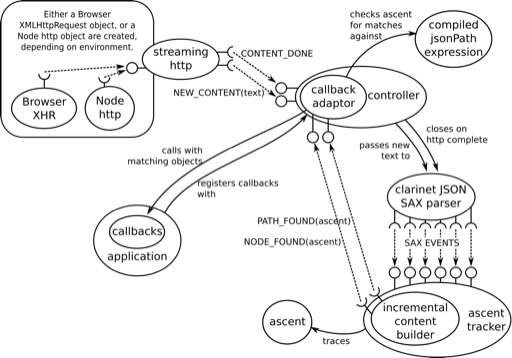
\includegraphics{images/overallDesign.png}
\caption{\textbf{Major components that make up Oboe.js} illustrating
program flow from http transport to registered callbacks. Every
component is not shown here. Particularly, components whose
responsibility it is to initialise the oboe instance but have no role
once it is running are omitted. UML facet/receptacle notation is used to
show the flow of events with event names in capitals.
\label{overallDesign}}
\end{figure}

Oboe's architecture has been designed to so that I may have as much
confidence as possible regarding the correct working of the library
through automated testing. Designing a system to be amenable to testing
in this case meant splitting into many co-operating parts each with an
easily specified remit.

Internally, communication between components is facilitated by an event
bus which is local to to Oboe instance. Most components interact solely
by picking up events, processing them and publishing further events in
response. Essentially, Oboe's architecture resembles a fairly linear
pipeline visiting a series of units, starting with http data and
sometimes ending with callbacks being notified. This use of an event bus
is a variation on the Observer pattern which removes the need for each
unit to obtain a reference to the previous one so that it may observe
it, giving a highly decoupled shape to the library. Once everything is
wired into the bus very little central control is required and the
larger behaviours emerge as the consequence of this interaction between
finer ones. One downside is perhaps that a central event bus does not
lend itself to a UML class diagram, giving a diagram shape with an event
bus as a central hub and everything else hanging off it as spokes.

\subsection{Automated testing}

Automated testing improves what can be written, not just making what is
written more reliable. Tests deal with the problem of ``irreducible
complexity'' - when a program is made out of parts whose correct
behaviour cannot be observed without all of the program. Allows smaller
units to be verified before verifying the whole.

\begin{figure}[htbp]
\centering
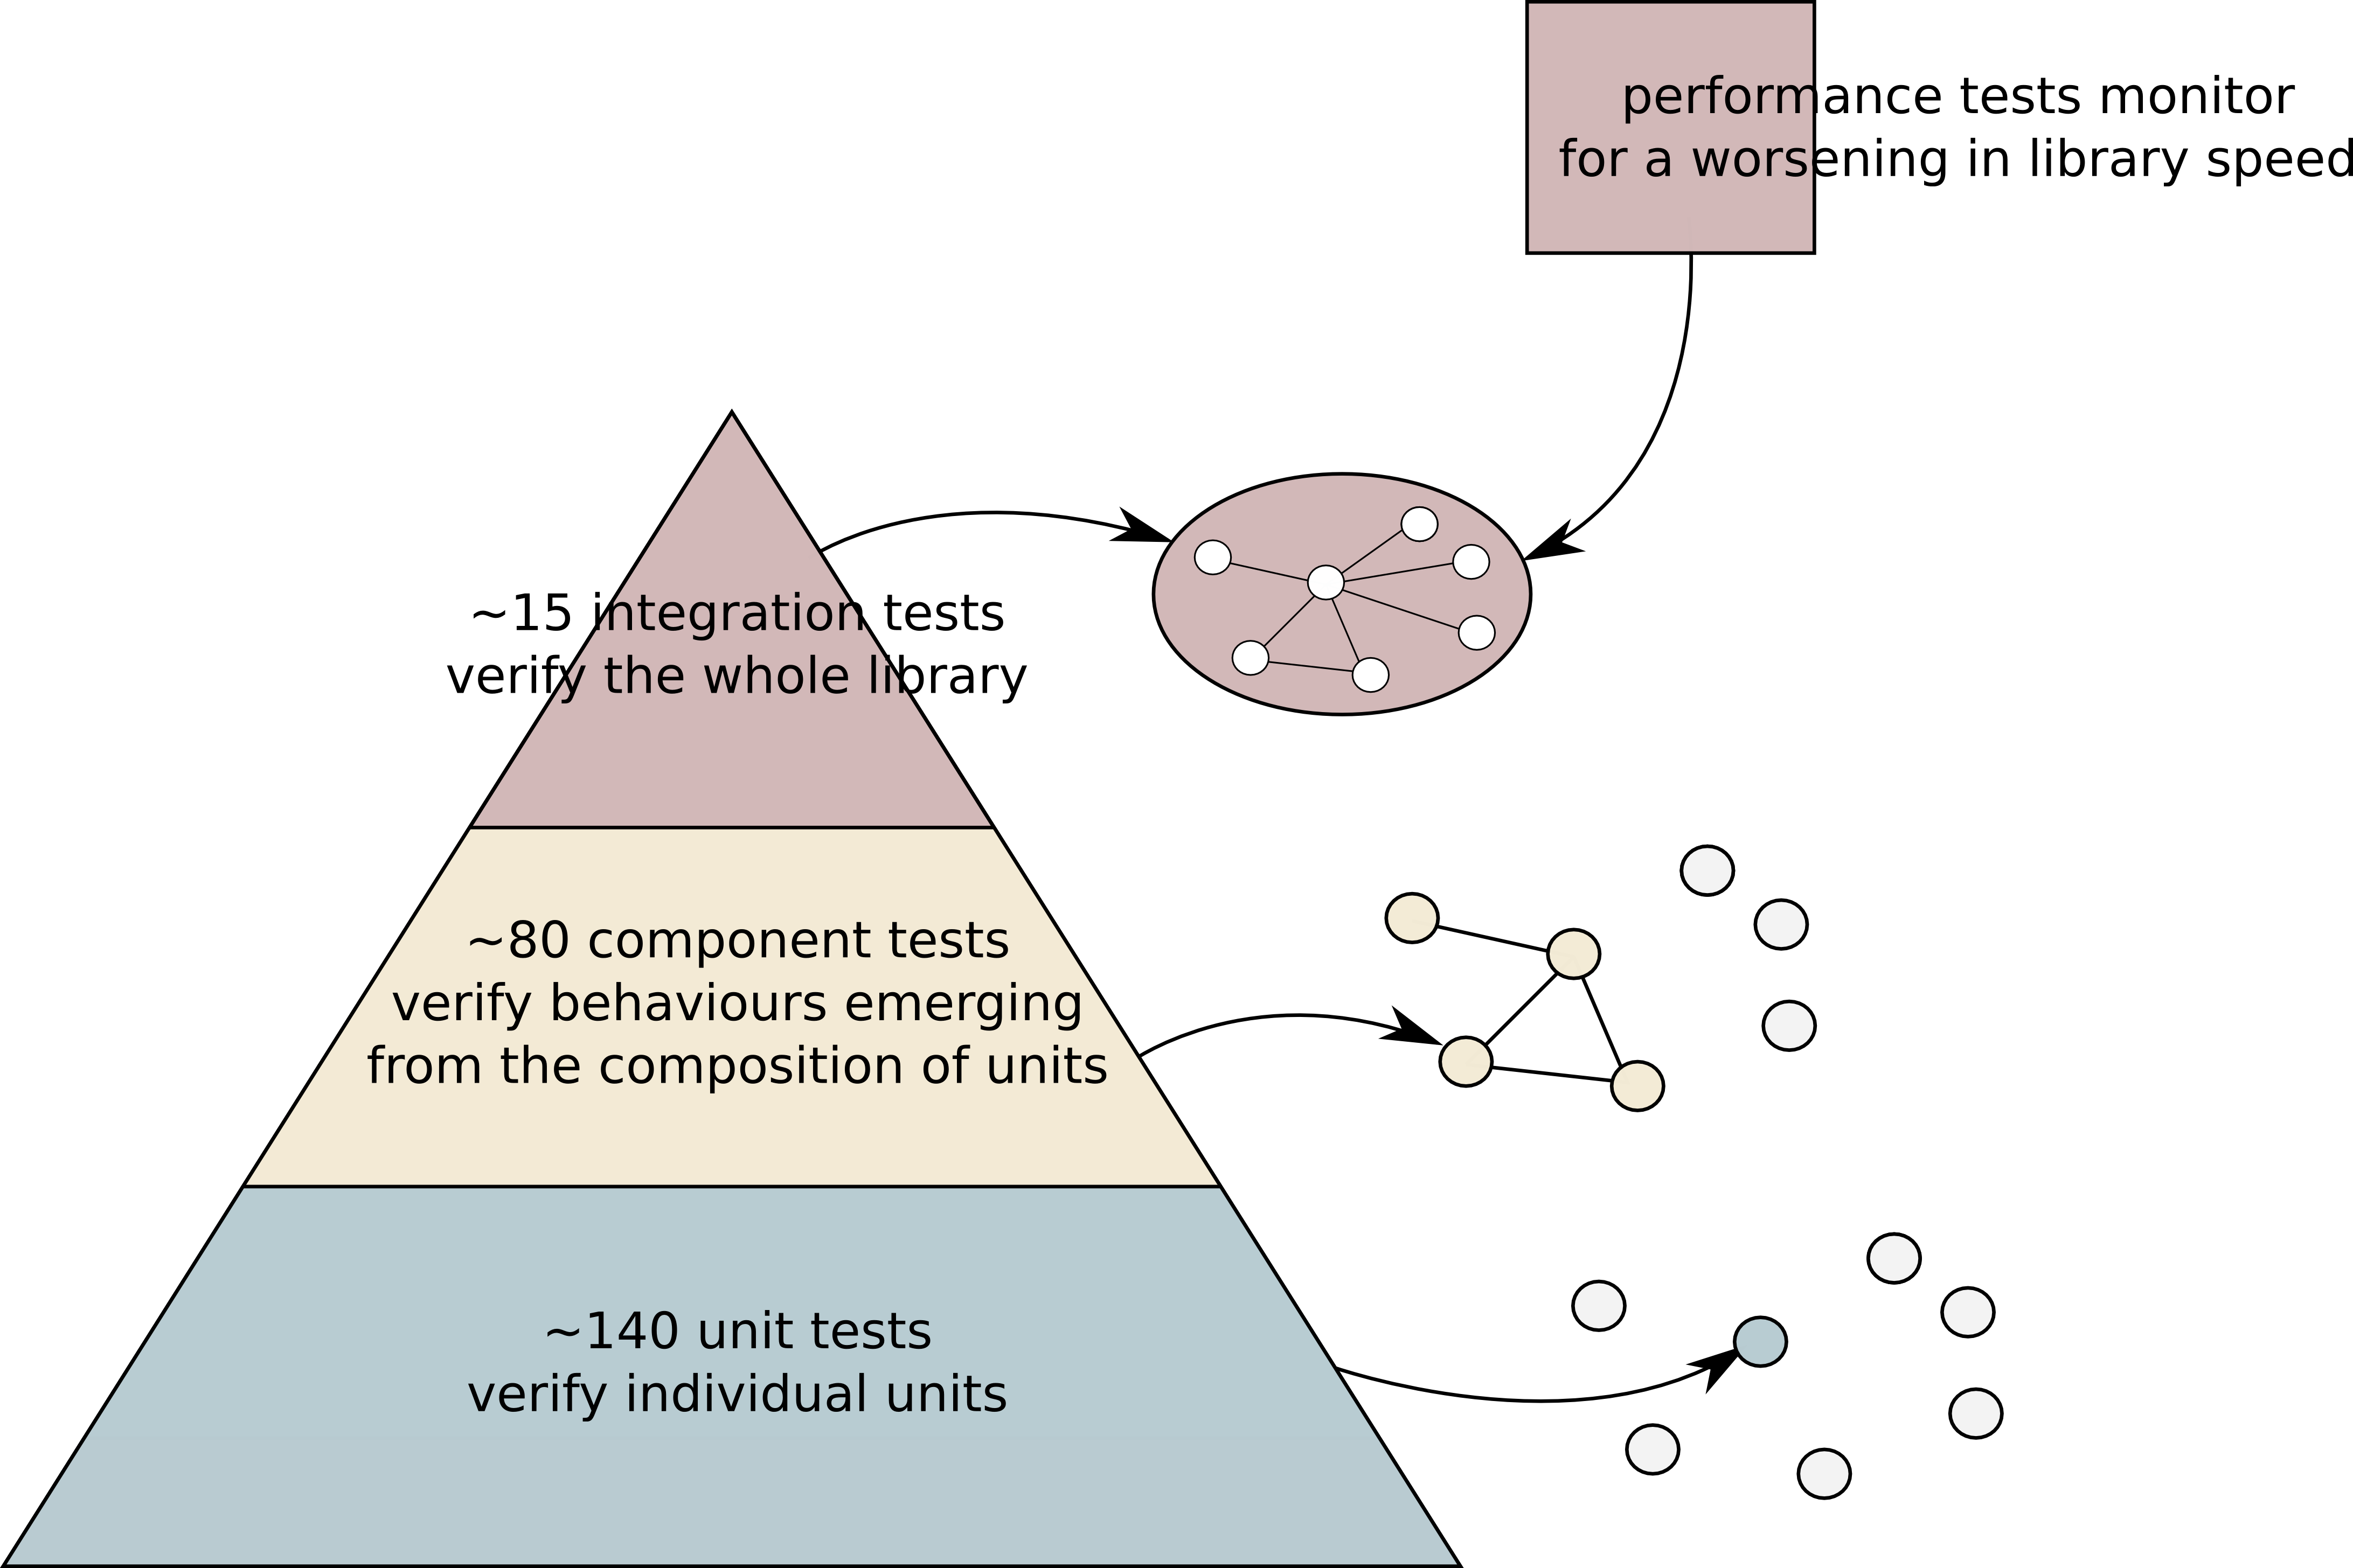
\includegraphics{images/testPyramid.png}
\caption{\textbf{The test pyramid}. Relying on the assumption that
verification of small parts provides a solid base from which to compose
system-level behaviours. A Lot of testing is done on the low-level
components of the system, less on the component level and less still on
a whole-system level where only smoke tests are provided.
\label{testpyramid}}
\end{figure}

The testing itself is a non-trivial undertaking with 80\% of code
written for this project being test specifications. Based on the idea
that a correct system must be built from individually correct units, the
majority of the specifications are unit tests, putting each unit under
the microscope and describing the correct behaviour as completely as
possible. Component tests zoom out from examining individual components
to focus on their correct composition, falsifying only the http traffic.
To avoid testing implementation details the component tests do not look
at the means of coupling between the code units but rather check for the
behaviours which should emerge as a consequence of their composition. At
the apex of the test pyramid are a small number of integration tests.
These verify Oboe as a black box without any knowledge of, or access to
the internals, using only the APIs which are exposed to application
programmers. When running the integration tests a REST service is first
spun up so that correctness of the whole library may be examined against
an actual server.

The desire to be amenable to testing influences the boundaries on which
the application splits into components. Confidently black box testing a
stateful unit as is difficult; because of side-effects it may later
react differently to the same calls. For this reason where state is
required it is stored in very simple state-storing units with intricate
program logic removed. The logic may then be separately expressed as
functions which map from one state to the next. Although comprehensive
coverage is of course impossible and tests are inevitably incomplete,
for whatever results the functions give while under test, uninfluenced
by state I can be sure that they will continue to give in any future
situation. The separate unit holding the state is trivial to test,
having exactly one responsibility: to store the result of a function
call and later pass that result to the next function. This approach
clearly breaks with object oriented style encapsulation by not hiding
data behind the logic which acts on them but I feel the departure is
worthwhile for the greater certainty it allows over the correct
functioning of the program.

Dual-implementation of same interface for streamingHttp might be
considered polymorphism, but a function not a class and both are never
loaded at run time.

Largely for the sake of testing Oboe has also embraced dependency
injection. This means that components do not create the further
components that they require but rather rely on them being provided by
an external wiring. The file \texttt{wire.js} performs the actual
injection. One such example is the streamingHttp component which hides
various incompatible http implementations by publishing their downloaded
content progressively via the event bus. This unit does not know how to
create the underlying browser XHR which it hides. Undoubtedly, by not
instantiating its own dependencies a it presents a less friendly
interface, although this is mitigated somewhat by the interface being
purely internal, the objects it depends on are no longer a hidden
implementation detail but exposed as a part of the component's API. The
advantage of dependency injection here is that unit testing is much
simpler. Unit tests should test exactly one behaviour of one unit. Were
the streaming http object to create its own transport, that part would
also be under test, plus whichever external service that it connects to.
Because Javascript allows redefinition of built in types, this could be
avoided by overwriting the XHR constructor to return a mock but
modifying the built in types for tests opens up the possibilities of
changes leaking between cases. Dependency injection allows a much
simpler test style because it is trivial to inject a stub in place of
the XHR.

Integration tests run against a node service which returns known content
according to known timings, somewhat emulating downloading via a slow
internet connection. For example, the url \texttt{/tenSlowNumbers}
writes out a JSON array of the first ten natural numbers at a rate of
one per second, while \texttt{/echoBackHeaders} writes back the http
headers that it received as a JSON object. The test specifications which
use these services interact with Oboe through the public API alone as an
application author would and try some tricky cases. For example,
requesting ten numbers but registering a listener against the fifth and
aborting the request on seeing it. The correct behaviour is to get no
callback for the sixth, even when running on platforms where the http is
buffered so that all ten will have already been downloaded. \emph{ref
apx for streamsource}

\subsection{Running the tests}

\begin{figure}[htbp]
\centering

\includegraphics{images/placeholder.png}
\caption{\textbf{Relationship between various files and test libraries}
\emph{other half of sketch from notebook}}
\end{figure}

The Grunt task runner was used to automate routine tasks such as
executing the tests and building. Unit and component tests run
automatically whenever a source file changes. As well as being correct
execution, the project is required to not surpass a certain size so the
built size is also checked. As a small, tightly focused project the
majority of programming is refactoring already working code. Running
tests on save provides quick feedback so that mistakes are found as soon
as they are made. Agile practitioners emphasise the importance of tests
that execute quickly (Martin 2008, T9), the 220 unit and component tests
run in less than a second so discovering mistakes is near instant. If
the ``content of any medium is always another medium'' (McLuhan 1964
p8), we might say that the content of programming is the program that is
realised by its execution. A person working in arts and crafts sees the
thing as they work but a programmer will usually not see the execution
simultaneously as they program. Conway observed that an artisan works by
transform-in-place ``start with the working material in place and you
step by step transform it into its final form'' whereas software is
created through intermediate proxies, and attempts to close this gap by
merging programming with the results of programming (Conway 2004
side8-9). When we bring together the medium and the message the cost of
small experimentation is very low and I feel that programming becomes
more explorative and expressive.

The integration tests are not run on save because they intentionally
simulate slow transfers and take some time to run. The integration tests
are used as a final check against built code before a branch in git can
be merged into the master. Once the code has been packaged for
distribution the internals are no longer visible the integration tests
which are coded against the public API are the only runnable tests.
While these tests don't individually test every component, they are
designed to exercise the whole codebase so that a mistake in any
component will be visible through them. Grunt executes the build,
including starting up the test REST services that give the integration
tests something to fetch.

\subsection{Packaging as a single, distributable file}

\begin{figure}[htbp]
\centering

\includegraphics{images/placeholder.png}
\caption{\textbf{Packaging of many javascript files into multiple
single-file packages.} The packages are individually targeted at
different execution contexts, either browsers or node \emph{get from
notebook, split sketch diagram in half}}
\end{figure}

As an interpreted language, Javascript may of course be ran directly
without any prior compilation. While running the same code as I see in
the editor is convenient while programming, it is much less so for
distribution. Although the languages imposes no compulsory build phase,
in practice one is necessary. Dependency managers have not yet become
standard for client-side web development (although Bower is looking
good) so most files are manually downloaded. For a developer wishing to
include my library in their own project a single file is much more
convenient. Should they not have a build process of their own, a single
file is also much faster to transfer to their users, mostly because of
the cost of establishing connections and the http overhead.

Javascript files are interpreted in series by the browser so load-time
dependencies must precede dependants. Unsurprisingly, separate files
once concatenated following the same order as delivered to the browser
will load more quickly but are functionally equivalent, at least barring
syntax errors. Several tools exist to automate this stage of the build
process, incorporating a topological sort of the dependency digraph in
order to find a working concatenation order.

Early in this project I chose \emph{Require.js} although I later moved
on because it was too heavyweight. Javascript as a language doesn't have
an import statement. Require contributes the importing ability to
Javascript from inside the language sandbox as the \texttt{require}
function, a standard asynchronous call. Calls to \texttt{require} AJAX
in and execute the imported source, returning any exported symbols by a
callback. For non-trivial applications this mode is intended mostly for
debugging; because a network hop is involved the protocol is chatty and
slowed by highly latent calls between modules. For efficient delivery
Require also has the \texttt{optimise} command which concatenates into a
single file by using static analysis to deduce a workable source order.
Because \texttt{require} may appear anywhere in the source, this in the
general case is of course undecidable so Require falls back to lazy
loading. In practice undecidability isn't a problem because imports are
generally not subject to branching. In larger webapps lazy loading
speeding up the initial page load and is actually an advantage. The
technique of \emph{Asynchronous Module Definition} (AMD) intentionally
imports rarely-loaded modules in response to events. By resisting the
static analysis the units will not be downloaded until they are needed.

AMD is mostly of interest to web applications with a central hub but
also some rarely used parts. Oboe does not fit this profile: everybody
who uses it will use all of the library. Regardless, I hoped to use
\texttt{optimise} to generate my combined Javascript file. Even after
optimisation, Require's design necessitates that calls to
\texttt{require} stay in the code and that the require.js run-time
component is available to handle these calls. For a micro-library a ???k
overhead was too large to accommodate. Overall, Require seems more
suited to developing stand-alone applications than programming
libraries.

Having abandoned Require, I decided to pick up the simplest tool which
could possibly work. With only 15 source files and a fairly sparse
dependency graph finding a working order on paper wasn't a daunting
task. Combined with a Grunt analogue to the unix \texttt{cat} command I
quickly had a working build process. I adjusted each Javascript file to,
when loaded directly, place its API in the global namespace, then
post-concatenation wrapped the combined in a single function, converting
the APIs inside the function from global to the scope of that function,
thereby hiding the implementation for code outside of Oboe.

For future consideration there is Browserify. This library reverses the
`browser first' image of Javascript by converting applications targeted
at Node into a single file efficiently packaged for delivery to a web
browser, conceptually making Node the primary environment for Javascript
and adapting browser execution to match. Significantly, require leaves
no trace of itself in the concatenated Javascript other than Adaptors
presenting browser APIs as the Node equivalents. Browserify's http
adaptor\footnote{\href{https://github.com/substack/http-browserify}{Https://github.com/substack/http-browserify}.}
is complete but more verbose compared to Oboe's version\footnote{\href{https://github.com/jimhigson/oboe.js/blob/master/src/streamingXhr.js}{Https://github.com/jimhigson/oboe.js/blob/master/src/streamingXhr.js}
  This version is shorter mostly because it is not a generic solution.}.

As well as combining into a single file, Javascript source can made
significantly smaller by removing comments and reducing inaccessible
tokens to a single character. For Oboe the popular library \emph{Uglify}
is used for minification. Uglify performs only surface optimisations,
operating on the AST level but concentrating mostly on compact syntax. I
also considered Google's Closure compiler. Closure resembles a
traditional compiler optimiser by leveraging a deeper understanding to
search for smaller representations, unfortunately at the cost of safety.
Decidability in highly dynamic languages is often impossible and Closure
operates on a well-advised subset of Javascript, delivering no
reasonable guarantee of equivalence when code is not written as the
Closure authors expected. Integration tests should catch any such
failures but for the time being I have a limited appetite for a workflow
which forces me to be suspicious of the project's build process.

\subsection{Styles of Programming}

The implementation of Oboe is mixed paradigm. Events flow throughout the
whole library but in terms of code style the components are a mix of
procedural, functional and object-oriented programming. Object
orientation is used only to wrap the library in an Object-oriented
public API and as a tuple-like store for multiple values. Constructors
are not used, nor is there any inheritance or notable polymorphism.
Closures, not objects, are used as the primary means of data storage and
hiding. Many of the entities painted in figure \ref{overallDesign} map
onto no single, addressable language construct and exist only as a set
of event handlers trapped inside the same closure, taking advantage of
the fact that their reachability from some event emitter prevents
required parameters from being garbage collected. From outside the
closure hidden values are not only private as would be seen in an OO
model, they are inherently unaddressable. Although only sparingly OO,
the high-level design's componentisation hasn't departed from how it
might be implemented in an OO metamodel and Object Oriented design
patterns remain influential despite being only loosely followed.

Because of the pressures on code size I decided not to use a general
purpose functional library and instead create my own with only the parts
that I need; see functional.js. Functional programming in Javascript is
known to be slower than other styles, particularly under Firefox because
it lacks Lambda Lifting and other similar optimisations (Guo 2013).
Considering to what degree performance concerns should dissuade us from
a functional style, we may consider the library's execution context.
Because of the single-threaded model any application's Javascript
execution is in between frames serving concurrent concerns so to
minimise the impact on latency for the other tasks it is important that
no task occupies the CPU for very long. On the browser about 16ms is a
fair maximum, allowing painting to occur at 60 frames per second. In
Node there is no hard limit but any CPU-hogging task degrades the
responsiveness of other responses. Context switching imposes a very low
overhead and responsive sharing generally proffers many small frames
over a few larger ones. In any case, server-side tasks especially are
more often i/o bound than CPU bound. Oboe's progressive design naturally
splits tasks which would otherwise be performed in a single frame over
many. For example, parsing and marshaling. Although the overall
computation may be higher, the total performance of the system should be
improved.

Javascript is of course an imperative language but over many iterations
Oboe has tended towards a declarative style. In
incrementalContentBuilder.js programming was initially stateful and
procedural, reading like the instructions to perform a task. Over many
refactors the flavour of the code has changed, the reading now tending
towards a description of desired behaviour.

\subsection{Incrementally building up the content}

As shown in figure \ref{overallDesign}, there is an incremental content
builder and ascent tracer which handle the output from the Clarinet JSON
SAX parser. Taken together, these might be considered a variant of the
Adaptor pattern, providing to the controller a simpler interface than is
presented by Clarinet. However, this is not the model implementation of
the pattern; the adapted interface is even-driven rather than
call-driven: we receive six kinds of event and in response emmit from a
narrower vocabulary of two.

To evaluate JSONPath expressions the controller requires a path to the
current JSON node, the node itself, and any ancestor nodes. This is
delivered by the incremental content builder as the payload of the
NODE\_FOUND and PATH\_FOUND events. For each Clarinet event the builder
provides a corresponding function which, working from the current path,
returns the next path after the event has been applied. For example, the
\texttt{objectopen} and \texttt{arrayopen} events move the current node
deeper in the document and are handled by adding new items to the path,
whereas for \texttt{closeobject} and \texttt{closearray} we remove one.
Over the course of parsing a complete JSON file the path will in this
way be manipulated to visit every node, allowing each to be tested
against the registered JSONPath expressions. Internally, the builder's
event handlers are declared as the combination of a smaller number of
basic reusable handler parts. Oboe is largely unconcerned regarding a
JSON node's type so given that several of the Clarinet events differ
only by the type of the nodes they announce, Oboe is able to generify
their handling by composing from a common pool of handler-parts. Picking
up \texttt{openobject} and \texttt{openarray} events, both fall through
to the same `nodeFound', differing only in a parameter. Similarly,
consider the \texttt{value} event which is fired when Clarinet
encounters a String or Number. Because primitive nodes are always leaves
the builder regards this as a node which instantaneously starts and
ends, handled programmatically as the functional composition of the
\texttt{nodeFound} and \texttt{curNodeFinished}. The reuse of smaller
instructions to build up larger ones is perhaps slightly reminiscent of
CISC CPU design in which micro-instructions are combined to implement
the chip's advertised interface.

Although the builder functions are stateless, ultimately the state
regarding the current path needs to be stored between clarinet calls.
This is handled by the ascent tracker. This tiny component merely serves
as a holder for this data, starting from an empty path it passes the
path to each builder function and stores the result to be given to the
next one.

\begin{figure}[htbp]
\centering
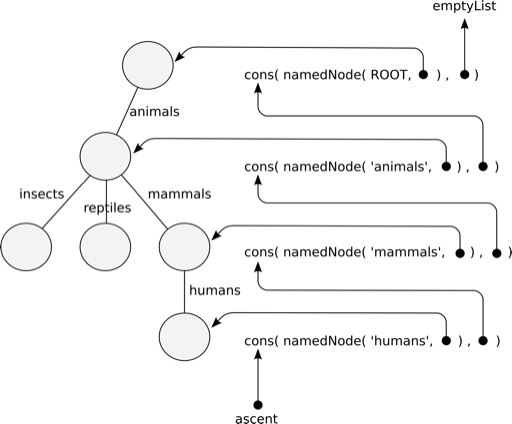
\includegraphics{images/ascent.png}
\caption{List representation of an ascent from leaf to root of a JSON
tree. Note the special ROOT token which represents the path mapping to
the root node (of course nothing maps to the root) - this is an object,
taking advantage of object identity to ensure that the token is unequal
to anything but itself. This list form is built up by the incremental
content builder and is the format that compiled JSONPath expressions
test against for matches \label{ascent}}
\end{figure}

The path of the current node is maintained as a singly linked list, with
each list element holding the field name and the node and the node
itself, see figure \ref{ascent}. The list is arranged with the JSON root
at the far end and the current node at the head. As we traverse the JSON
the current node is appended and removed many times whereas the root is
immutable. This ordering was chosen because it is computationally very
efficient since all updates to the list are at the head. Each link in
the list is immutable, enforced by newer Javascript engines as frozen
objects.\footnote{See
  \url{https://developer.mozilla.org/en-US/docs/Web/JavaScript/Reference/Global\textbackslash{}_Objects/Object/freeze}.
  Although older engines don't provide any ability to create immutable
  objects at run-time, we can be fairly certain that the code does not
  mutate these objects or the tests would fail when run in environments
  which are able to enforce this.}

Linked lists were chosen in preference to the more conventional approach
of using native Javascript Arrays for several reasons. Firstly, I find
this area of the program more easy to test and debug given immutable
data structures. Handling native Arrays without mutating would be very
expensive because on each new path the array would have to be copied
rather than edited in-place. Unpicking a stack trace is easier if I know
that every value revealed is the value that has always occupied that
space because I don't have to think four-dimensionally projecting my
mind forwards and back in time to different values that were there when
the variable was used. The lack of side effects means I can try explore
new commands in the debugger's CLI without worrying about breaking the
execution of the program. Most Javascript virtual machines are also
quite poor at array growing and shrinking so for collections whose size
changes often are outperformed by linked lists. Finally, this is a very
convenient format for the JSONPath engine to perform matching on as will
be discussed in the next section. The Javascript file lists.js
implements the list functions: \texttt{cons}, \texttt{head},
\texttt{tail}, \texttt{map}, \texttt{foldR}, \texttt{all}.

Because it is more common to quote paths as descents rather than ascent,
on the boundary to the outside world Oboe reverses the order and,
because Javascript programmers will not be familiar with this structure,
converts to arrays.

\subsection{Oboe JSONPath Implementation}

Not surprisingly given its importance, the JSONPath implementation is
one of the most refactored and considered parts of the Oboe codebase.
Like many small languages, on the first commit it was little more than a
series of regular expressions\footnote{JSONPath compiler from the first
  commit can be found at line 159 here:
  \url{https://github.com/jimhigson/oboe.js/blob/a17db7accc3a371853a2a0fd755153b10994c91e/src/main/progressive.js}\#L159.}
but has slowly evolved into a featureful and efficient
implementation\footnote{For contrast, the current source can be found at
  \url{https://github.com/jimhigson/oboe.js/blob/master/src/jsonPath.js}.}.
The extent of the rewriting was possible because the correct behaviour
is well defined by test specifications\footnote{The current tests are
  viewable at
  \url{https://github.com/jimhigson/oboe.js/blob/master/test/specs/jsonPath.unit.spec.js}
  and
  \url{https://github.com/jimhigson/oboe.js/blob/master/test/specs/jsonPathTokens.unit.spec.js}.}.

The JSONPath compiler exposes a single higher-order function to the rest
of Oboe. This function takes a JSONPath as a String and, proving it is a
valid expression, returns a function which tests for matches to the
JSONPath. Both the compiler and the functions that it generates benefit
from being stateless. The type of the compiler, expressed as Haskell
syntax would be:

\begin{Shaded}
\begin{Highlighting}[]
\DataTypeTok{String} \OtherTok{->} \DataTypeTok{Ascent} \OtherTok{->} \DataTypeTok{JsonPathMatchResult}
\end{Highlighting}
\end{Shaded}

The match result is either a failure to match, or a hit, with the node
that matched. In the case of path matching, the node may currently be
unknown. If the pattern has a clause prefixed with \texttt{\$}, the node
matching that clause is captured and returned as the result. Otherwise,
the last clause is implicitly capturing.

The usage profile for JSONPath expressions in Oboe is to be compiled
once and then evaluated many times, once for each node encountered while
parsing the JSON. Because matching is performed perhaps hundreds of
times per file the most pressing performance consideration is for
matching to execute quickly, the time required to compile is relatively
unimportant. Oboe's JSONPath design contrasts with JSONPath's reference
implementation which, because it provides a first order function,
freshly reinterprets the JSONPath string each time it is invoked.

The compilation is performed by recursively by examining the left-most
side of the string for a JSONPath clause. For each kind of clause there
is a function which matches ascents against that clause, for example by
checking the name field. By partial completion this function is
specialised to match against one particular name. Once a clause function
is generated, compilation recurs by passing to itself the remaining
unparsed portion of the JSONPath string. This continues until it is
called with a zero-length JSONPath. On each recursive call the clause
function is wrapped in the result from the next recursive call,
resulting ultimately in a linked series of clause functions. When
evaluated against an ascent, each clause functions examines the head of
the ascent and passes the ascent onto the next function if it passes. A
special clause functions, \texttt{skip1} is used for the \texttt{.}
syntax and places no condition on the head of the ascent but passes on
to the next clause only the tail, thus moving evaluation of the ascent
one node up the parsed JSON tree. Similarly, there is a
\texttt{skipMany} which maps onto the \texttt{..} syntax and recursively
consumes nodes until it can find a match in the next clause.

JsonPath implementation allows the compilation of complex expressions
into an executable form, but each part implementing the executable form
is locally simple. By using recursion, assembling the simple functions
into a more function expressing a more complex rule also follows as
being locally simple but gaining a usefully sophisticated behaviour
through composition of simple parts. Each recursive call of the parser
identifies one token for non-empty input and then recursively digests
the rest.

As an example, the pattern \texttt{!.\$person..\{height tShirtSize\}}
once compiled would roughly resemble the Javascript functional
representation below:

\begin{Shaded}
\begin{Highlighting}[]
\FunctionTok{statementExpr}\NormalTok{(             }\CommentTok{// wrapper, added when JSONPath is zero-length }
   \FunctionTok{duckTypeClause}\NormalTok{(         }\CommentTok{// token 6, \{height tShirtSize\}}
      \FunctionTok{skipMany}\NormalTok{(            }\CommentTok{// token 5, '..'  }
         \FunctionTok{capture}\NormalTok{(          }\CommentTok{// token 4, css4-style '$' notation}
            \FunctionTok{nameClause}\NormalTok{(    }\CommentTok{// token 3, 'person'}
               \FunctionTok{skip1}\NormalTok{(      }\CommentTok{// token 2, '.'  }
                  \NormalTok{rootExpr }\CommentTok{// token 1, '!' at start of JSONPath expression}
               \NormalTok{) }
            \StringTok{'person'} \NormalTok{)}
         \NormalTok{)}
   \NormalTok{), [}\StringTok{'height'}\NormalTok{, }\StringTok{'tShirtSize'}\NormalTok{])}
\NormalTok{)      }
\end{Highlighting}
\end{Shaded}

Since I am only using a side-effect free subset of Javascript for this
segment of Oboe it would be safe to use a functional cache. As well as
saving time by avoiding repeated execution, this could potentially also
save memory because where two JSONPath strings contain a common start
they could share the inner parts of their functional expression.
Although Javascript doesn't come with functional caching, it can be
added using the language itself.\footnote{Probably the best known
  example being \texttt{memoize} from Underscore.js:
  \url{http://underscorejs.org/}\#memoize.} I suspect, however, that
hashing the parameters might be slower than performing the matching.
Although the parameters are all immutable and could in theory be hashed
by object identity, in practice there is no way to access an object id
from inside the language so any hash of a node parsed out of JSON would
have to walk the entire subtree rooted from that node.

The JSONPath tokenisation is split out into its own file and separately
tested. The tokenisation implementation is based on regular expressions,
they are the simplest form able to express the clause patterns. The
regular expressions are hidden to the outside the tokenizer and only
functions are exposed to the main body of the compiler. The regular
expressions all start with \texttt{\^{}} so that they only match at the
head of the string. A more elegant alternative is the `y'\footnote{\href{https://developer.mozilla.org/en-US/docs/Web/JavaScript/Guide/Regular\textbackslash{}_Expressions}{Https://developer.mozilla.org/en-US/docs/Web/JavaScript/Guide/Regular\textbackslash{}\_Expressions}.}
flag but as of now this lacks wide browser support.

By verifying the tokens through their own unit tests it is simpler to
thoroughly specify the tokenisation, producing simpler failure messages
than if it were done through the full JSONPath engine. We might consider
the unit test layer of the pyramid (figure \ref{testpyramid}) is further
split into two sub-layers. Arguably, the upper of these sub-layer is not
a unit test because it is verifying two units together. There is some
redundancy with the tokens being tested both individually and as full
expressions. I maintain that this is the best approach regardless
because stubbing out the tokenizer functions would be a considerable
effort and would not improve the rigor of the JSONPath specification.

\begin{figure}[htbp]
\centering

\includegraphics{images/placeholder.png}
\caption{Some kind of diagram showing jsonPath expressions and functions
partially completed to link back to the previous function. Include the
statementExpr pointing to the last clause}
\end{figure}

\section{Conclusion}

\subsection{Benchmarking vs non-progressive REST}

I feel it is important to experimentally answer the question, \emph{is
this actually any faster?}. To do this I have created a small
benchmarking suite that runs under Node.js. I chose Node because it at
its code is a very basic platform which I feel it gives a more
repeatable environment than modern browsers which at during the tests
could be performing any number of background tasks. These tests may be
seen in the \texttt{benchmark} folder of the project. Node also has the
advantage in measuring the memory of a running process is not swamped by
the memory taken up by the browser itself.

One of the proposed advantages of progressive REST is an improved user
experience because of earlier, more progressive interface rendering and
a perceptual improvement in speed. I am not focusing on this area for
benchmarking because it would be much more difficult to measure,
involving human participants. While I can't provide numbers on the
perceptual improvements, I have created sites using Oboe and the
improvement in responsiveness over slower networks is large enough to be
obvious.

The benchmark mimics a relational database-backed REST service.
Relational databases serve data to a cursor one tuple at a time. The
simulated service writes out twenty tuples as JSON objects, one every
ten milliseconds. To simulate network slowness, Apple's \emph{Network
Line Conditioner} was used. I chose the named presets ``3G, Average
Case'' and ``Cable modem'' to represent poor and good networks
respectively.\footnote{\href{http://mattgemmell.com/2011/07/25/network-link-conditioner-in-lion/}{Http://mattgemmell.com/2011/07/25/network-link-conditioner-in-lion/}.}
Each test involves two node processes, one acting as the client and one
as the server, with data transfer between them via normal http.

Memory was measured using Node's built in memory reporting tool,
\texttt{process.memoryusage()} and the maximum figure returned on each
run was taken

Each object in the returned JSON contains a URL to a further resource.
Each further resource is fetched and parsed. The aggregation is complete
when we have them all.

\begin{longtable}[c]{@{}llrrr@{}}
\hline\noalign{\medskip}
Strategy & Network & First output (ms) & Total time (ms) & Max. Memory
(Mb)
\\\noalign{\medskip}
\hline\noalign{\medskip}
Oboe.js & Good & 40 & 804 & 6.2
\\\noalign{\medskip}
Oboe.js & Poor & 60 & 1,526 & 6.2
\\\noalign{\medskip}
JSON.parse (DOM) & Good & 984 & 1,064 & 9,0
\\\noalign{\medskip}
JSON.parse (DOM) & Poor & 2550 & 2,609 & 8.9
\\\noalign{\medskip}
Clarinet (SAX) & Good & 34 & 781 & 5.5
\\\noalign{\medskip}
Clarinet (SAX) & Poor & 52 & 1,510 & 5.5
\\\noalign{\medskip}
\hline
\end{longtable}

Vs Json.parse shows a dramatic improvement over first output of about
96\% and a smaller but significant improvement of about 40\% in time
required to complete the task. Oboe's performance in terms of time is
about 15\% slower than Clarinet; since Oboe is built on Clarinet it
could not be faster but I had hoped for these results to be closer.

As expected, in this simulation of real-world usage, the extra
computation\\compared to JSON.parse which is needed by Oboe's more
involved algorithms or Clarinet's less efficient parsing\footnote{\href{http://writings.nunojob.com/2011/12/clarinet-sax-based-evented-streaming-json-parser-in-javascript-for-the-browser-and-nodejs.html}{Http://writings.nunojob.com/2011/12/clarinet-sax-based-evented-streaming-json-parser-in-javascript-for-the-browser-and-nodejs.html}.}
have been dwarfed by better i/o management. Reacting earlier using
slower handlers has been shown to be faster overall than reacting later
with quicker ones. I believe that this vindicates a focus on efficient
management of i/o over faster algorithms. I believe that much
programming takes a ``Hurry up and wait'' approach by concentrating
overly on optimal computation rather than optimal i/o management.

There is an unexpected improvement vs JSON.parse in terms of memory
usage. It is not clear why this would be but it may be attributable to
the json fetching library used to simplify the JSON.parse tests having a
large dependency tree. As expected, Clarinet shows the largest
improvements in terms of memory usage. For very large JSON I would
expect Clarinet's memory usage to remain roughly constant whilst the two
approaches rise linearly with the size of the resource.

\subsection{Comparative Programmer Ergonomics}

For each of the benchmarks above the code was laid out in the most
natural way for the strategy under test.

\begin{longtable}[c]{@{}lrr@{}}
\hline\noalign{\medskip}
Strategy & Code Required (lines) & Code required (chars)
\\\noalign{\medskip}
\hline\noalign{\medskip}
Oboe.js & 3 & 64
\\\noalign{\medskip}
JSON.parse & 5 & 102
\\\noalign{\medskip}
Clarinet (SAX) & 30 & lots!
\\\noalign{\medskip}
\hline
\end{longtable}

Oboe was the shortest:

\begin{Shaded}
\begin{Highlighting}[]
\FunctionTok{oboe}\NormalTok{(DB_URL).}\FunctionTok{node}\NormalTok{(}\StringTok{'\{id url\}.url'}\NormalTok{, }\KeywordTok{function}\NormalTok{(url)\{}
        
   \FunctionTok{oboe}\NormalTok{(url).}\FunctionTok{node}\NormalTok{(}\StringTok{'name'}\NormalTok{, }\KeywordTok{function}\NormalTok{(name)\{}
                   
      \OtherTok{console}\NormalTok{.}\FunctionTok{log}\NormalTok{(name);               }
   \NormalTok{\});      }
\NormalTok{\});}
\end{Highlighting}
\end{Shaded}

Non-progressive parsing was slightly longer, requiring in addition a
loop, an if statement, and programmatically selecting specific parts of
the results:

\begin{Shaded}
\begin{Highlighting}[]
\CommentTok{// JSON.parse. The code is shortened and simplified by get-json from NPM:}
\CommentTok{// https://npmjs.org/package/get-json}

\FunctionTok{getJson}\NormalTok{(DB_URL, }\KeywordTok{function}\NormalTok{(err, records) \{}
    
   \OtherTok{records}\NormalTok{.}\OtherTok{data}\NormalTok{.}\FunctionTok{forEach}\NormalTok{( }\KeywordTok{function}\NormalTok{( record )\{}
    
      \KeywordTok{if}\NormalTok{( }\OtherTok{record}\NormalTok{.}\FunctionTok{url} \NormalTok{) \{}
      
         \FunctionTok{getJson}\NormalTok{(}\OtherTok{record}\NormalTok{.}\FunctionTok{url}\NormalTok{, }\KeywordTok{function}\NormalTok{(err, record) \{}
         
            \OtherTok{console}\NormalTok{.}\FunctionTok{log}\NormalTok{(}\OtherTok{record}\NormalTok{.}\FunctionTok{name}\NormalTok{);}
         \NormalTok{\});}
      \NormalTok{\}}
   \NormalTok{\});}
\NormalTok{\});}
\end{Highlighting}
\end{Shaded}

The JSON.parse version is very closely coupled with the format that it
is handling. We can see this in the fragments \texttt{records.data},
\texttt{record.url}, \texttt{record.name} which expects to find
sub-trees at very specific locations in the JSON. The code might be said
to contain a description of the format that it is for. Conversely, the
Oboe version describes the format only so far as is needed to identify
the parts that it is interested in; the remainder of the format could
change and the code would continue to work. As well as being simpler to
program against than the previous simplest mode, I believe this
demonstrates a greater tolerance to changing formats.

The Clarinet version of the code may be seen in appendex (??). This
version is greater in verbosity and obfuscation. I don't think a person
could look at this source and understand what is being parsed without
thinking about it for a long time. Parameter names such as `key' or
`value' must be chosen by the position of the token in the markup, prior
to understanding the semantics it represents. By contrast, Oboe and
JSON.parse both allow names to be given by the meaning of the token.

\subsection{Performance of code styles under various engines}

The 15\% overhead of Oboe vs Clarinet suggests Oboe might be
computationally expensive. With very fast networks the extra computation
might outweigh a more efficient i/o strategy.

The file \texttt{test/specs/oboe.performance.spec.js} contains a simple
benchmark. This test registeres a very complex JSONPath expression which
intentionally uses all of the language and fetches a JSON file
containing 100 objects, each with 8 String properties against .
Correspondingly the expression is evaluated just over 800 times and 100
matches are found. Although real http is used, it is kept within the
localhost. The results below are averaged from ten runs. The tests
executed on a Macbook Air, except for Chrome Mobile which was tested on
an iPhone 5. Tests requiring Microsoft Windows were performed inside a
virtual machine.

Curl is a simple download to stdout from the shell and is included as a
control run to provide a baseline.

\begin{longtable}[c]{@{}lll@{}}
\hline\noalign{\medskip}
Platform & Total Time & Throughput (nodes per ms)
\\\noalign{\medskip}
\hline\noalign{\medskip}
Curl (control) & 42ms & \emph{n/a}
\\\noalign{\medskip}
Node.js v0.10.1 & 172ms & 4.67
\\\noalign{\medskip}
Chrome 30.0.1599 (Mac OS X 10.7.5) & 202ms & 3.98
\\\noalign{\medskip}
Safari 6.0.5 (Mac OS X 10.7.5) & 231ms & 3.48
\\\noalign{\medskip}
IE 10.0.0 (Windows 8) & 349ms & 2.30
\\\noalign{\medskip}
Chrome Mobile iOS 30.0.1599 (iOS 7.0.2) & 431ms & 1.86
\\\noalign{\medskip}
Firefox 24.0.0 (Mac OS X 10.7) & 547ms & 1.47
\\\noalign{\medskip}
IE 8.0.0 (Windows XP) & 3,048ms & 0.26
\\\noalign{\medskip}
\hline
\end{longtable}

We can see that Firefox is much slower than other modern browsers
despite its SpiderMonkey Javascript engine being normally quite fast.
This is probably explicable in part by SpiderMonkey's just-in-time
compiler being poor at optimising functional Javascript (Guo 2013).
Because the JSON nodes are not of a common type the related callsites
are not monomorphic which Firefox also optimises poorly (Guo 2013). When
the test was repeated using a simpler JSONPath expression Firefox showed
by far the largest improvement indicating that on this platform the
functional pattern matching is the bottleneck.

Of these results I find only the very low performance on old versions of
Internet Explorer concerning, almost certainly degrading user experience
more than it is improved. It might be reasonable to conclude that for
complex use cases Oboe is currently not unsuited to legacy platforms.
Since this platform cannot progressively interpret an XHR response, if
performance on legacy platforms becomes a serious concern one option
might be to create a non-progressive library with the same API which
could be selectively delivered to those platforms in place of the main
version.

Nonetheless, in its current form Oboe may slow down the total time when
working over the very fastest connections.

For an imperative language coded in a functional style the compiler may
not optimise as effectively as if a functional language was used. This
is especially the case under a highly dynamic language in which
everything, even the built-in constructs are mutable. I think Javascript
was a good choice of language given it is already well adopted and
allows the targeting of server and client side with only minimal effort,
giving a very large number of applications with the potential to adopt
Oboe. However, there are obvious inefficiencies such as the the descent
and ancestor arrays which are always created to be handed to application
callbacks but that I anticipate will be predominantly ignored. The
design of Oboe is very amicable to implementation under a functional
language and it would be interesting to see the results.

\subsection{Status as a micro-library}

Built versions of Oboe as delivered reside in the project's
\texttt{dist} folder. The file \texttt{oboe-browser.min.js} is the
minified version which should be sent to browsers gzipped. After gzip is
applied this file comes to 4966 bytes; close to but comfortably under
the 5120 limit. At roughly the size as a very small image, the size of
Oboe should not discourage adoption.

\subsection{potential future work}

There is nothing about Oboe which precludes working with other
tree-shaped format. If there is demand, An XML/XPATH version seems like
an obvious expansion. Currently Oboe only operates on http traffic.
While this restriction is reasonable in a Browser context, under Node it
is unnecessarily limiting and should be lifted by allowing arbitrary
streams to be read.

Oboe stores all items that are parsed from the JSON it receives,
resulting in a memory use which is as high as a DOM parser. These are
kept in order to be able to provide a match to any possible JSONPath
expression. However, in most cases memory would be saved if the parsed
content were only stored so far as is needed to provide matches against
the JSONPath expressions which have actually been registered. For
typical use cases I expect this would allow the non-storage of large
branches. Likewise, the current implementation takes a rather brute
force approach when examining node for pattern matches: check every
registered JSONPath expression against every node and path that are
found in the JSON. For many expressions we are able to know there is no
possibility of matching a JSON tree, either because we have already
matched or because the the current node's ancestors already mandate
failure. A more sophisticated programme might disregard provably
unsatisfiable handlers for the duration of a subtree. Either of these
changes would involve some rather difficult programming and because
matching is fast enough I think brute force is the best approach for the
time being.

During JSONPath matching much of the computation is repeated. For
example, matching the expression \texttt{b.*} against many children of a
common parent will repeat the same test, checking if the parent's name
is `b', for each child node. Because the JSONPath matching is stateless,
recursive and side-effect free there is a potential to cut out repeated
computation by using a functional cache. This would reduce the overall
amount of computation needed for JSONPath expressions with common
substrings to their left side or nodes with a common ancestry. Current
Javascript implementations make it difficult to manage a functional
cache, or caches in general, from inside the language itself because
there is no way to occupy only the unused memory. Weak references are
proposed in ECMAScript 6 but currently only experimentally
supported\footnote{At time of writing, Firefox is the only engine
  supporting WeakHashMap by default. In Chome it is implemented but not
  available to Javascript unless explicitly enabled by a browser flag.
  \url{https://developer.mozilla.org/en-US/docs/Web/JavaScript/Reference/Global\textbackslash{}_Objects/WeakMap}
  retrieved 11th October 2013.}. For future development they would be
ideal.

The nodes which Oboe hands to callbacks are mutable meaning that
potentially the correct workings of the library could be broken if the
containing application carelessly alters them. Newer implementations of
Javascript allows a whole object to be made immutable, or just certain
properties via an immutability decorator and the \texttt{defineProperty}
method. This would probably be an improvement.

\hyperdef{}{appendix_http_limits}{\section{Appendix i: Limits to number
of simultaneous connections under various http
clients}\label{appendix_http_limits}}

\begin{longtable}[c]{@{}ll@{}}
\hline\noalign{\medskip}
\begin{minipage}[b]{0.22\columnwidth}\raggedright
http Client
\end{minipage} & \begin{minipage}[b]{0.29\columnwidth}\raggedright
connection limit per server
\end{minipage}
\\\noalign{\medskip}
\hline\noalign{\medskip}
\begin{minipage}[t]{0.22\columnwidth}\raggedright
Firefox
\end{minipage} & \begin{minipage}[t]{0.29\columnwidth}\raggedright
6
\end{minipage}
\\\noalign{\medskip}
\begin{minipage}[t]{0.22\columnwidth}\raggedright
Internet Explorer
\end{minipage} & \begin{minipage}[t]{0.29\columnwidth}\raggedright
4
\end{minipage}
\\\noalign{\medskip}
\begin{minipage}[t]{0.22\columnwidth}\raggedright
Chrome / Chromium
\end{minipage} & \begin{minipage}[t]{0.29\columnwidth}\raggedright
32 sockets per proxy 6 sockets per destination host 256 sockets per
process
\end{minipage}
\\\noalign{\medskip}
\hline
\end{longtable}

\url{https://developer.mozilla.org/en-US/docs/Web/API/XMLHttpRequest}

\url{http://msdn.microsoft.com/de-de/magazine/ee330731.aspx}\#http11\_max\_con

\url{http://dev.chromium.org/developers/design-documents/network-stack}\#TOC-Connection-Management

\section{Appendix ii: Oboe.js source code listing}

\subsection{clarinetListenerAdaptor.js}

\begin{Shaded}
\begin{Highlighting}[]

\CommentTok{/** }
\CommentTok{ * A bridge used to assign stateless functions to listen to clarinet.}
\CommentTok{ * }
\CommentTok{ * As well as the parameter from clarinet, each callback will also be passed}
\CommentTok{ * the result of the last callback.}
\CommentTok{ * }
\CommentTok{ * This may also be used to clear all listeners by assigning zero handlers:}
\CommentTok{ * }
\CommentTok{ *    clarinetListenerAdaptor( clarinet, \{\} )}
\CommentTok{ */}
\KeywordTok{function} \FunctionTok{clarinetListenerAdaptor}\NormalTok{(clarinetParser, handlers)\{}
    
   \KeywordTok{var} \NormalTok{state;}

   \OtherTok{clarinet}\NormalTok{.}\OtherTok{EVENTS}\NormalTok{.}\FunctionTok{forEach}\NormalTok{(}\KeywordTok{function}\NormalTok{(eventName)\{}
 
      \KeywordTok{var} \NormalTok{handlerFunction = handlers[eventName];}
      
      \NormalTok{clarinetParser[}\StringTok{'on'}\NormalTok{+eventName] = handlerFunction && }
                                       \KeywordTok{function}\NormalTok{(param) \{}
                                          \NormalTok{state = }\FunctionTok{handlerFunction}\NormalTok{( state, param);}
                                       \NormalTok{\};}
   \NormalTok{\});}
\NormalTok{\}}
\end{Highlighting}
\end{Shaded}

\pagebreak

\subsection{events.js}

\begin{Shaded}
\begin{Highlighting}[]
\CommentTok{/**}
\CommentTok{ * This file declares some constants to use as names for event types.}
\CommentTok{ */}

\KeywordTok{var} \CommentTok{// NODE_FOUND, PATH_FOUND and ERROR_EVENT feature }
    \CommentTok{// in the public API via .on('node', ...) or .on('path', ...)}
    \CommentTok{// so these events are strings}
    \NormalTok{NODE_FOUND    = }\StringTok{'node'}\NormalTok{,  }
    \NormalTok{PATH_FOUND    = }\StringTok{'path'}\NormalTok{,   }
         
    \CommentTok{// these events are never exported so are kept as }
    \CommentTok{// the smallest possible representation, numbers:}
    \NormalTok{_S = }\DecValTok{0}\NormalTok{,}
    \NormalTok{ERROR_EVENT   = _S++,    }
    \NormalTok{ROOT_FOUND    = _S++,    }
    \NormalTok{NEW_CONTENT = _S++,}
    \NormalTok{END_OF_CONTENT = _S++,}
    \NormalTok{ABORTING = _S++;}
\end{Highlighting}
\end{Shaded}

\pagebreak

\subsection{functional.js}

\begin{Shaded}
\begin{Highlighting}[]
\CommentTok{/** }
\CommentTok{ * Partially complete a function.}
\CommentTok{ * }
\CommentTok{ * Eg: }
\CommentTok{ *    var add3 = partialComplete( function add(a,b)\{return a+b\}, [3] );}
\CommentTok{ *    }
\CommentTok{ *    add3(4) // gives 7}
\CommentTok{ */}
\KeywordTok{var} \NormalTok{partialComplete = }\FunctionTok{varArgs}\NormalTok{(}\KeywordTok{function}\NormalTok{( fn, boundArgs ) \{}

      \KeywordTok{return} \FunctionTok{varArgs}\NormalTok{(}\KeywordTok{function}\NormalTok{( callArgs ) \{}
               
         \KeywordTok{return} \OtherTok{fn}\NormalTok{.}\FunctionTok{apply}\NormalTok{(}\KeywordTok{this}\NormalTok{, }\OtherTok{boundArgs}\NormalTok{.}\FunctionTok{concat}\NormalTok{(callArgs));}
      \NormalTok{\}); }
   \NormalTok{\}),}


\CommentTok{/**}
\CommentTok{ * Compose zero or more functions:}
\CommentTok{ * }
\CommentTok{ *    compose(f1, f2, f3)(x) = f1(f2(f3(x))))}
\CommentTok{ * }
\CommentTok{ * The last (inner-most) function may take more than one parameter:}
\CommentTok{ * }
\CommentTok{ *    compose(f1, f2, f3)(x,y) = f1(f2(f3(x,y))))}
\CommentTok{ */}
   \NormalTok{compose = }\FunctionTok{varArgs}\NormalTok{(}\KeywordTok{function}\NormalTok{(fns) \{}

      \KeywordTok{var} \NormalTok{fnsList = }\FunctionTok{arrayAsList}\NormalTok{(fns);}
   
      \KeywordTok{function} \FunctionTok{next}\NormalTok{(params, curFn) \{  }
         \KeywordTok{return} \NormalTok{[}\FunctionTok{apply}\NormalTok{(params, curFn)];   }
      \NormalTok{\}}
      
      \KeywordTok{return} \FunctionTok{varArgs}\NormalTok{(}\KeywordTok{function}\NormalTok{(startParams)\{}
        
         \KeywordTok{return} \FunctionTok{foldR}\NormalTok{(next, startParams, fnsList)[}\DecValTok{0}\NormalTok{];}
      \NormalTok{\});}
   \NormalTok{\}),}

\CommentTok{/**}
\CommentTok{ * Call a list of functions with the same args until one returns a }
\CommentTok{ * truthy result. Similar to the \textbar{}\textbar{} operator.}
\CommentTok{ * }
\CommentTok{ * So:}
\CommentTok{ *      lazyUnion([f1,f2,f3 ... fn])( p1, p2 ... pn )}
\CommentTok{ *      }
\CommentTok{ * Is equivalent to: }
\CommentTok{ *      apply([p1, p2 ... pn], f1) \textbar{}\textbar{} }
\CommentTok{ *      apply([p1, p2 ... pn], f2) \textbar{}\textbar{} }
\CommentTok{ *      apply([p1, p2 ... pn], f3) ... apply(fn, [p1, p2 ... pn])  }
\CommentTok{ *  }
\CommentTok{ * }\KeywordTok{@returns}\CommentTok{ the first return value that is given that is truthy.}
\CommentTok{ */}
   \NormalTok{lazyUnion = }\FunctionTok{varArgs}\NormalTok{(}\KeywordTok{function}\NormalTok{(fns) \{}

      \KeywordTok{return} \FunctionTok{varArgs}\NormalTok{(}\KeywordTok{function}\NormalTok{(params)\{}
   
         \KeywordTok{var} \NormalTok{maybeValue;}
   
         \KeywordTok{for} \NormalTok{(}\KeywordTok{var} \NormalTok{i = }\DecValTok{0}\NormalTok{; i < }\FunctionTok{len}\NormalTok{(fns); i++) \{}
   
            \NormalTok{maybeValue = }\FunctionTok{apply}\NormalTok{(params, fns[i]);}
   
            \KeywordTok{if}\NormalTok{( maybeValue ) \{}
               \KeywordTok{return} \NormalTok{maybeValue;}
            \NormalTok{\}}
         \NormalTok{\}}
      \NormalTok{\});}
   \NormalTok{\});   }

\CommentTok{/**}
\CommentTok{ * This file declares various pieces of functional programming.}
\CommentTok{ * }
\CommentTok{ * This isn't a general purpose functional library, to keep things small it}
\CommentTok{ * has just the parts useful for Oboe.js.}
\CommentTok{ */}


\CommentTok{/**}
\CommentTok{ * Call a single function with the given arguments array.}
\CommentTok{ * Basically, a functional-style version of the OO-style Function#apply for }
\CommentTok{ * when we don't care about the context ('this') of the call.}
\CommentTok{ * }
\CommentTok{ * The order of arguments allows partial completion of the arguments array}
\CommentTok{ */}
\KeywordTok{function} \FunctionTok{apply}\NormalTok{(args, fn) \{}
   \KeywordTok{return} \OtherTok{fn}\NormalTok{.}\FunctionTok{apply}\NormalTok{(}\KeywordTok{undefined}\NormalTok{, args);}
\NormalTok{\}}

\CommentTok{/**}
\CommentTok{ * Define variable argument functions but cut out all that tedious messing about }
\CommentTok{ * with the arguments object. Delivers the variable-length part of the arguments}
\CommentTok{ * list as an array.}
\CommentTok{ * }
\CommentTok{ * Eg:}
\CommentTok{ * }
\CommentTok{ * var myFunction = varArgs(}
\CommentTok{ *    function( fixedArgument, otherFixedArgument, variableNumberOfArguments )\{}
\CommentTok{ *       console.log( variableNumberOfArguments );}
\CommentTok{ *    \}}
\CommentTok{ * )}
\CommentTok{ * }
\CommentTok{ * myFunction('a', 'b', 1, 2, 3); // logs [1,2,3]}
\CommentTok{ * }
\CommentTok{ * var myOtherFunction = varArgs(function( variableNumberOfArguments )\{}
\CommentTok{ *    console.log( variableNumberOfArguments );}
\CommentTok{ * \})}
\CommentTok{ * }
\CommentTok{ * myFunction(1, 2, 3); // logs [1,2,3]}
\CommentTok{ * }
\CommentTok{ */}
\KeywordTok{function} \FunctionTok{varArgs}\NormalTok{(fn)\{}

   \KeywordTok{var} \NormalTok{numberOfFixedArguments = }\OtherTok{fn}\NormalTok{.}\FunctionTok{length} \NormalTok{-}\DecValTok{1}\NormalTok{;}
         
   \KeywordTok{return} \KeywordTok{function}\NormalTok{()\{}
   
      \KeywordTok{var} \NormalTok{numberOfVaraibleArguments = }\OtherTok{arguments}\NormalTok{.}\FunctionTok{length} \NormalTok{- numberOfFixedArguments,}
      
          \NormalTok{argumentsToFunction = }\OtherTok{Array}\NormalTok{.}\OtherTok{prototype}\NormalTok{.}\OtherTok{slice}\NormalTok{.}\FunctionTok{call}\NormalTok{(arguments);}
          
      \CommentTok{// remove the last n element from the array and append it onto the end of}
      \CommentTok{// itself as a sub-array}
      \OtherTok{argumentsToFunction}\NormalTok{.}\FunctionTok{push}\NormalTok{( }
         \OtherTok{argumentsToFunction}\NormalTok{.}\FunctionTok{splice}\NormalTok{(numberOfFixedArguments, numberOfVaraibleArguments)}
      \NormalTok{);   }
      
      \KeywordTok{return} \OtherTok{fn}\NormalTok{.}\FunctionTok{apply}\NormalTok{( }\KeywordTok{this}\NormalTok{, argumentsToFunction );}
   \NormalTok{\}       }
\NormalTok{\}}


\CommentTok{/**}
\CommentTok{ * Swap the order of parameters to a binary function}
\CommentTok{ * }
\CommentTok{ * A bit like this flip: http://zvon.org/other/haskell/Outputprelude/flip_f.html}
\CommentTok{ */}
\KeywordTok{function} \FunctionTok{flip}\NormalTok{(fn)\{}
   \KeywordTok{return} \KeywordTok{function}\NormalTok{(a, b)\{}
      \KeywordTok{return} \FunctionTok{fn}\NormalTok{(b,a);}
   \NormalTok{\}}
\NormalTok{\}}


\CommentTok{/**}
\CommentTok{ * Create a function which is the intersection of two other functions.}
\CommentTok{ * }
\CommentTok{ * Like the && operator, if the first is truthy, the second is never called,}
\CommentTok{ * otherwise the return value from the second is returned.}
\CommentTok{ */}
\KeywordTok{function} \FunctionTok{lazyIntersection}\NormalTok{(fn1, fn2) \{}

   \KeywordTok{return} \KeywordTok{function} \NormalTok{(param) \{}
                                                              
      \KeywordTok{return} \FunctionTok{fn1}\NormalTok{(param) && }\FunctionTok{fn2}\NormalTok{(param);}
   \NormalTok{\};   }
\NormalTok{\}}

\end{Highlighting}
\end{Shaded}

\pagebreak

\subsection{incrementalContentBuilder.js}

\begin{Shaded}
\begin{Highlighting}[]
\CommentTok{/** }
\CommentTok{ * This file provides various listeners which can be used to build up}
\CommentTok{ * a changing ascent based on the callbacks provided by Clarinet. It listens}
\CommentTok{ * to the low-level events from Clarinet and fires higher-level ones.}
\CommentTok{ *  }
\CommentTok{ * The building up is stateless so to track a JSON file}
\CommentTok{ * clarinetListenerAdaptor.js is required to store the ascent state}
\CommentTok{ * between calls.}
\CommentTok{ */}


\KeywordTok{var} \NormalTok{keyOf = }\FunctionTok{attr}\NormalTok{(}\StringTok{'key'}\NormalTok{);}
\KeywordTok{var} \NormalTok{nodeOf = }\FunctionTok{attr}\NormalTok{(}\StringTok{'node'}\NormalTok{);}


\CommentTok{/** }
\CommentTok{ * A special value to use in the path list to represent the path 'to' a root }
\CommentTok{ * object (which doesn't really have any path). This prevents the need for }
\CommentTok{ * special-casing detection of the root object and allows it to be treated }
\CommentTok{ * like any other object. We might think of this as being similar to the }
\CommentTok{ * 'unnamed root' domain ".", eg if I go to }
\CommentTok{ * http://en.wikipedia.org./wiki/En/Main_page the dot after 'org' deliminates }
\CommentTok{ * the unnamed root of the DNS.}
\CommentTok{ * }
\CommentTok{ * This is kept as an object to take advantage that in Javascript's OO objects }
\CommentTok{ * are guaranteed to be distinct, therefore no other object can possibly clash }
\CommentTok{ * with this one. Strings, numbers etc provide no such guarantee. }
\CommentTok{ **/}
\KeywordTok{var} \NormalTok{ROOT_PATH = \{\};}


\CommentTok{/**}
\CommentTok{ * Create a new set of handlers for clarinet's events, bound to the fire }
\CommentTok{ * function given.  }
\CommentTok{ */} 
\KeywordTok{function} \FunctionTok{incrementalContentBuilder}\NormalTok{( fire) \{}


   \KeywordTok{function} \FunctionTok{arrayIndicesAreKeys}\NormalTok{( possiblyInconsistentAscent, newDeepestNode) \{}
   
      \CommentTok{/* for values in arrays we aren't pre-warned of the coming paths }
\CommentTok{         (Clarinet gives no call to onkey like it does for values in objects) }
\CommentTok{         so if we are in an array we need to create this path ourselves. The }
\CommentTok{         key will be len(parentNode) because array keys are always sequential }
\CommentTok{         numbers. */}

      \KeywordTok{var} \NormalTok{parentNode = }\FunctionTok{nodeOf}\NormalTok{( }\FunctionTok{head}\NormalTok{( possiblyInconsistentAscent));}
      
      \KeywordTok{return}      \FunctionTok{isOfType}\NormalTok{( Array, parentNode)}
               \NormalTok{?}
                  \FunctionTok{pathFound}\NormalTok{(  possiblyInconsistentAscent, }
                              \FunctionTok{len}\NormalTok{(parentNode), }
                              \NormalTok{newDeepestNode}
                  \NormalTok{)}
               \NormalTok{:  }
                  \CommentTok{// nothing needed, return unchanged}
                  \NormalTok{possiblyInconsistentAscent }
               \NormalTok{;}
   \NormalTok{\}}
                 
   \KeywordTok{function} \FunctionTok{nodeFound}\NormalTok{( ascent, newDeepestNode ) \{}
      
      \KeywordTok{if}\NormalTok{( !ascent ) \{}
         \CommentTok{// we discovered the root node,}
         \FunctionTok{fire}\NormalTok{( ROOT_FOUND, newDeepestNode);}
                    
         \KeywordTok{return} \FunctionTok{pathFound}\NormalTok{( ascent, ROOT_PATH, newDeepestNode);         }
      \NormalTok{\}}

      \CommentTok{// we discovered a non-root node}
                 
      \KeywordTok{var} \NormalTok{arrayConsistentAscent  = }\FunctionTok{arrayIndicesAreKeys}\NormalTok{( ascent, newDeepestNode),      }
          \NormalTok{ancestorBranches       = }\FunctionTok{tail}\NormalTok{( arrayConsistentAscent),}
          \NormalTok{previouslyUnmappedName = }\FunctionTok{keyOf}\NormalTok{( }\FunctionTok{head}\NormalTok{( arrayConsistentAscent));}
          
      \FunctionTok{appendBuiltContent}\NormalTok{( }
         \NormalTok{ancestorBranches, }
         \NormalTok{previouslyUnmappedName, }
         \NormalTok{newDeepestNode }
      \NormalTok{);}
                                                                                                         
      \KeywordTok{return} \FunctionTok{cons}\NormalTok{( }
               \FunctionTok{namedNode}\NormalTok{( previouslyUnmappedName, newDeepestNode ), }
               \NormalTok{ancestorBranches}
      \NormalTok{);                                                                          }
   \NormalTok{\}}


   \CommentTok{/**}
\CommentTok{    * Add a new value to the object we are building up to represent the}
\CommentTok{    * parsed JSON}
\CommentTok{    */}
   \KeywordTok{function} \FunctionTok{appendBuiltContent}\NormalTok{( ancestorBranches, key, node )\{}
     
      \FunctionTok{nodeOf}\NormalTok{( }\FunctionTok{head}\NormalTok{( ancestorBranches))[key] = node;}
   \NormalTok{\}}

   \CommentTok{/**}
\CommentTok{    * Get a new key->node mapping}
\CommentTok{    * }
\CommentTok{    * }\KeywordTok{@param}\CommentTok{ }\KeywordTok{\{String\textbar{}Number\}}\CommentTok{ key}
\CommentTok{    * }\KeywordTok{@param}\CommentTok{ }\KeywordTok{\{Object\textbar{}Array\textbar{}String\textbar{}Number\textbar{}null\}}\CommentTok{ node a value found in the json}
\CommentTok{    */}
   \KeywordTok{function} \FunctionTok{namedNode}\NormalTok{(key, node) \{}
      \KeywordTok{return} \NormalTok{\{}\DataTypeTok{key}\NormalTok{:key, }\DataTypeTok{node}\NormalTok{:node\};}
   \NormalTok{\}}
     
   \CommentTok{/**}
\CommentTok{    * For when we find a new key in the json.}
\CommentTok{    * }
\CommentTok{    * }\KeywordTok{@param}\CommentTok{ }\KeywordTok{\{String\textbar{}Number\textbar{}Object\}}\CommentTok{ newDeepestName the key. If we are in an }
\CommentTok{    *    array will be a number, otherwise a string. May take the special }
\CommentTok{    *    value ROOT_PATH if the root node has just been found}
\CommentTok{    *    }
\CommentTok{    * }\KeywordTok{@param}\CommentTok{ }\KeywordTok{\{String\textbar{}Number\textbar{}Object\textbar{}Array\textbar{}Null\textbar{}undefined\}}\CommentTok{ [maybeNewDeepestNode] }
\CommentTok{    *    usually this won't be known so can be undefined. Can't use null }
\CommentTok{    *    to represent unknown because null is a valid value in JSON}
\CommentTok{    **/}  
   \KeywordTok{function} \FunctionTok{pathFound}\NormalTok{(ascent, newDeepestName, maybeNewDeepestNode) \{}

      \KeywordTok{if}\NormalTok{( ascent ) \{ }\CommentTok{// if not root}
      
         \CommentTok{// If we have the key but (unless adding to an array) no known value}
         \CommentTok{// yet. Put that key in the output but against no defined value:      }
         \FunctionTok{appendBuiltContent}\NormalTok{( ascent, newDeepestName, maybeNewDeepestNode );}
      \NormalTok{\}}
   
      \KeywordTok{var} \NormalTok{ascentWithNewPath = }\FunctionTok{cons}\NormalTok{( }
                                 \FunctionTok{namedNode}\NormalTok{( newDeepestName, }
                                            \NormalTok{maybeNewDeepestNode), }
                                 \NormalTok{ascent}
                              \NormalTok{);}
     
      \FunctionTok{fire}\NormalTok{( PATH_FOUND, ascentWithNewPath);}
 
      \KeywordTok{return} \NormalTok{ascentWithNewPath;}
   \NormalTok{\}}


   \CommentTok{/**}
\CommentTok{    * For when the current node ends}
\CommentTok{    */}
   \KeywordTok{function} \FunctionTok{curNodeFinished}\NormalTok{( ascent ) \{}

      \FunctionTok{fire}\NormalTok{( NODE_FOUND, ascent);}
                          
      \CommentTok{// pop the complete node and its path off the list:                                    }
      \KeywordTok{return} \FunctionTok{tail}\NormalTok{( ascent);}
   \NormalTok{\}      }
                 
   \KeywordTok{return} \NormalTok{\{ }

      \DataTypeTok{openobject }\NormalTok{: }\KeywordTok{function} \NormalTok{(ascent, firstKey) \{}

         \KeywordTok{var} \NormalTok{ascentAfterNodeFound = }\FunctionTok{nodeFound}\NormalTok{(ascent, \{\});         }

         \CommentTok{/* It is a perculiarity of Clarinet that for non-empty objects it}
\CommentTok{            gives the first key with the openobject event instead of}
\CommentTok{            in a subsequent key event.}
\CommentTok{                      }
\CommentTok{            firstKey could be the empty string in a JSON object like }
\CommentTok{            \{'':'foo'\} which is technically valid.}
\CommentTok{            }
\CommentTok{            So can't check with !firstKey, have to see if has any }
\CommentTok{            defined value. */}
         \KeywordTok{return} \FunctionTok{defined}\NormalTok{(firstKey)}
         \NormalTok{?          }
            \CommentTok{/* We know the first key of the newly parsed object. Notify that }
\CommentTok{               path has been found but don't put firstKey permanently onto }
\CommentTok{               pathList yet because we haven't identified what is at that key }
\CommentTok{               yet. Give null as the value because we haven't seen that far }
\CommentTok{               into the json yet */}
            \FunctionTok{pathFound}\NormalTok{(ascentAfterNodeFound, firstKey)}
         \NormalTok{:}
            \NormalTok{ascentAfterNodeFound}
         \NormalTok{;}
      \NormalTok{\},}
    
      \DataTypeTok{openarray}\NormalTok{: }\KeywordTok{function} \NormalTok{(ascent) \{}
         \KeywordTok{return} \FunctionTok{nodeFound}\NormalTok{(ascent, []);}
      \NormalTok{\},}

      \CommentTok{// called by Clarinet when keys are found in objects               }
      \DataTypeTok{key}\NormalTok{: pathFound,}
      
      \CommentTok{/* Emitted by Clarinet when primitive values are found, ie Strings,}
\CommentTok{         Numbers, and null.}
\CommentTok{         Because these are always leaves in the JSON, we find and finish the }
\CommentTok{         node in one step, expressed as functional composition: */}
      \DataTypeTok{value}\NormalTok{: }\FunctionTok{compose}\NormalTok{( curNodeFinished, nodeFound ),}
      
      \CommentTok{// we make no distinction in how we handle object and arrays closing.}
      \CommentTok{// For both, interpret as the end of the current node.}
      \DataTypeTok{closeobject}\NormalTok{: curNodeFinished,}
      \DataTypeTok{closearray}\NormalTok{: curNodeFinished       }
   \NormalTok{\};}
\NormalTok{\}}
\end{Highlighting}
\end{Shaded}

\pagebreak

\subsection{instanceController.js}

\begin{Shaded}
\begin{Highlighting}[]
\CommentTok{/**}
\CommentTok{ * This file implements a light-touch central controller for an instance }
\CommentTok{ * of Oboe which provides the methods used for interacting with the instance }
\CommentTok{ * from the calling app.}
\CommentTok{ */}
 
 
\KeywordTok{function} \FunctionTok{instanceController}\NormalTok{(fire, on, clarinetParser, contentBuilderHandlers) \{}
  
   \KeywordTok{var} \NormalTok{oboeApi, rootNode;}

   \CommentTok{// when the root node is found grap a reference to it for later      }
   \FunctionTok{on}\NormalTok{(ROOT_FOUND, }\KeywordTok{function}\NormalTok{(root) \{}
      \NormalTok{rootNode = root;   }
   \NormalTok{\});}
                              
   \FunctionTok{on}\NormalTok{(NEW_CONTENT,         }
      \KeywordTok{function} \NormalTok{(nextDrip) \{}
         \CommentTok{// callback for when a bit more data arrives from the streaming XHR         }
          
         \KeywordTok{try} \NormalTok{\{}
            
            \OtherTok{clarinetParser}\NormalTok{.}\FunctionTok{write}\NormalTok{(nextDrip);            }
         \NormalTok{\} }\KeywordTok{catch}\NormalTok{(e) \{ }
            \CommentTok{/* we don't have to do anything here because we always assign}
\CommentTok{               a .onerror to clarinet which will have already been called }
\CommentTok{               by the time this exception is thrown. */}                
         \NormalTok{\}}
      \NormalTok{\}}
   \NormalTok{);}
   
   \CommentTok{/* At the end of the http content close the clarinet parser.}
\CommentTok{      This will provide an error if the total content provided was not }
\CommentTok{      valid json, ie if not all arrays, objects and Strings closed properly */}
   \FunctionTok{on}\NormalTok{(END_OF_CONTENT, }\OtherTok{clarinetParser}\NormalTok{.}\OtherTok{close}\NormalTok{.}\FunctionTok{bind}\NormalTok{(clarinetParser));}
   

   \CommentTok{/* If we abort this Oboe's request stop listening to the clarinet parser. }
\CommentTok{      This prevents more tokens being found after we abort in the case where }
\CommentTok{      we aborted during processing of an already filled buffer. */}
   \FunctionTok{on}\NormalTok{( ABORTING, }\KeywordTok{function}\NormalTok{() \{}
      \FunctionTok{clarinetListenerAdaptor}\NormalTok{(clarinetParser, \{\});}
   \NormalTok{\});   }

   \FunctionTok{clarinetListenerAdaptor}\NormalTok{(clarinetParser, contentBuilderHandlers);}
  
   \CommentTok{// react to errors by putting them on the event bus}
   \OtherTok{clarinetParser}\NormalTok{.}\FunctionTok{onerror} \NormalTok{= }\KeywordTok{function}\NormalTok{(e) \{          }
      \FunctionTok{fire}\NormalTok{(ERROR_EVENT, e);}
      
      \CommentTok{// note: don't close clarinet here because if it was not expecting}
      \CommentTok{// end of the json it will throw an error}
   \NormalTok{\};}

   \KeywordTok{function} \FunctionTok{addPathOrNodeCallback}\NormalTok{( eventId, pattern, callback ) \{}
   
      \KeywordTok{var} \NormalTok{matchesJsonPath = }\FunctionTok{jsonPathCompiler}\NormalTok{( pattern );}
   
      \CommentTok{// Add a new callback adaptor to the eventBus.}
      \CommentTok{// This listener first checks that he pattern matches then if it does, }
      \CommentTok{// passes it onto the callback. }
      \FunctionTok{on}\NormalTok{( eventId, }\KeywordTok{function}\NormalTok{( ascent )\{ }
 
         \KeywordTok{var} \NormalTok{maybeMatchingMapping = }\FunctionTok{matchesJsonPath}\NormalTok{( ascent );}
     
         \CommentTok{/* Possible values for maybeMatchingMapping are now:}

\CommentTok{            false: }
\CommentTok{               we did not match }
\CommentTok{  }
\CommentTok{            an object/array/string/number/null: }
\CommentTok{               we matched and have the node that matched.}
\CommentTok{               Because nulls are valid json values this can be null.}
\CommentTok{  }
\CommentTok{            undefined: }
\CommentTok{               we matched but don't have the matching node yet.}
\CommentTok{               ie, we know there is an upcoming node that matches but we }
\CommentTok{               can't say anything else about it. }
\CommentTok{         */}
         \KeywordTok{if}\NormalTok{( maybeMatchingMapping !== }\KeywordTok{false} \NormalTok{) \{                                 }

            \FunctionTok{notifyCallback}\NormalTok{(callback, maybeMatchingMapping, ascent);                           }
         \NormalTok{\}}
      \NormalTok{\});   }
   \NormalTok{\}   }
   
   \KeywordTok{function} \FunctionTok{notifyCallback}\NormalTok{(callback, matchingMapping, ascent) \{}
      \CommentTok{/* }
\CommentTok{         We're now calling back to outside of oboe where the Lisp-style }
\CommentTok{         lists that we are using internally will not be recognised }
\CommentTok{         so convert to standard arrays. }
\CommentTok{  }
\CommentTok{         Also, reverse the order because it is more common to list paths }
\CommentTok{         "root to leaf" than "leaf to root" }
\CommentTok{      */}
            
      \KeywordTok{var} \NormalTok{descent     = }\FunctionTok{reverseList}\NormalTok{(ascent),}
      
          \CommentTok{// To make a path, strip off the last item which is the special}
          \CommentTok{// ROOT_PATH token for the 'path' to the root node}
          \NormalTok{path       = }\FunctionTok{listAsArray}\NormalTok{(}\FunctionTok{tail}\NormalTok{(}\FunctionTok{map}\NormalTok{(keyOf,descent))),}
          \NormalTok{ancestors  = }\FunctionTok{listAsArray}\NormalTok{(}\FunctionTok{map}\NormalTok{(nodeOf, descent)); }
      
      \KeywordTok{try}\NormalTok{\{}
      
         \FunctionTok{callback}\NormalTok{( }\FunctionTok{nodeOf}\NormalTok{(matchingMapping), path, ancestors );   }
      \NormalTok{\}}\KeywordTok{catch}\NormalTok{(e)  \{}
      
         \CommentTok{// An error occured during the callback, publish it on the event bus }
         \FunctionTok{fire}\NormalTok{(ERROR_EVENT, e);}
      \NormalTok{\}          }
   \NormalTok{\}}

   \CommentTok{/**}
\CommentTok{    * Add several listeners at a time, from a map}
\CommentTok{    */}
   \KeywordTok{function} \FunctionTok{addListenersMap}\NormalTok{(eventId, listenerMap) \{}
   
      \KeywordTok{for}\NormalTok{( }\KeywordTok{var} \NormalTok{pattern }\KeywordTok{in} \NormalTok{listenerMap ) \{}
         \FunctionTok{addPathOrNodeCallback}\NormalTok{(eventId, pattern, listenerMap[pattern]);}
      \NormalTok{\}}
   \NormalTok{\}    }
      
   \CommentTok{/**}
\CommentTok{    * implementation behind .onPath() and .onNode()}
\CommentTok{    */}       
   \KeywordTok{function} \FunctionTok{addNodeOrPathListenerApi}\NormalTok{( eventId, jsonPathOrListenerMap,}
                                      \NormalTok{callback, callbackContext )\{}
 
      \KeywordTok{if}\NormalTok{( }\FunctionTok{isString}\NormalTok{(jsonPathOrListenerMap) ) \{}
         \FunctionTok{addPathOrNodeCallback}\NormalTok{( }
            \NormalTok{eventId, }
            \NormalTok{jsonPathOrListenerMap, }
            \OtherTok{callback}\NormalTok{.}\FunctionTok{bind}\NormalTok{(callbackContext\textbar{}\textbar{}oboeApi)}
         \NormalTok{);}
      \NormalTok{\} }\KeywordTok{else} \NormalTok{\{}
         \FunctionTok{addListenersMap}\NormalTok{(eventId, jsonPathOrListenerMap);}
      \NormalTok{\}}
      
      \KeywordTok{return} \KeywordTok{this}\NormalTok{; }\CommentTok{// chaining}
   \NormalTok{\}}

   \CommentTok{/**}
\CommentTok{    * Construct and return the public API of the Oboe instance to be }
\CommentTok{    * returned to the calling application}
\CommentTok{    */}
   \KeywordTok{return} \NormalTok{oboeApi = \{ }
      \DataTypeTok{path  }\NormalTok{:  }\FunctionTok{partialComplete}\NormalTok{(addNodeOrPathListenerApi, PATH_FOUND), }
      \DataTypeTok{node  }\NormalTok{:  }\FunctionTok{partialComplete}\NormalTok{(addNodeOrPathListenerApi, NODE_FOUND),}
      \DataTypeTok{on    }\NormalTok{:  addNodeOrPathListenerApi,}
      \DataTypeTok{fail  }\NormalTok{:  }\FunctionTok{partialComplete}\NormalTok{(on, ERROR_EVENT),}
      \DataTypeTok{done  }\NormalTok{:  }\FunctionTok{partialComplete}\NormalTok{(addNodeOrPathListenerApi, NODE_FOUND, }\StringTok{'!'}\NormalTok{),}
      \DataTypeTok{abort }\NormalTok{:  }\FunctionTok{partialComplete}\NormalTok{(fire, ABORTING),}
      \DataTypeTok{root  }\NormalTok{:  }\KeywordTok{function} \FunctionTok{rootNodeFunctor}\NormalTok{() \{}
                  \KeywordTok{return} \NormalTok{rootNode;}
               \NormalTok{\}}
   \NormalTok{\};}
\NormalTok{\}}
\end{Highlighting}
\end{Shaded}

\pagebreak

\subsection{jsonPath.js}

\begin{Shaded}
\begin{Highlighting}[]
\CommentTok{/**}
\CommentTok{ * The jsonPath evaluator compiler used for Oboe.js. }
\CommentTok{ * }
\CommentTok{ * One function is exposed. This function takes a String JSONPath spec and }
\CommentTok{ * returns a function to test candidate ascents for matches.}
\CommentTok{ * }
\CommentTok{ *  String jsonPath -> (List ascent) -> Boolean\textbar{}Object}
\CommentTok{ *}
\CommentTok{ * This file is coded in a pure functional style. That is, no function has }
\CommentTok{ * side effects, every function evaluates to the same value for the same }
\CommentTok{ * arguments and no variables are reassigned.}
\CommentTok{ */}  
\CommentTok{// the call to jsonPathSyntax injects the token syntaxes that are needed }
\CommentTok{// inside the compiler}
\KeywordTok{var} \NormalTok{jsonPathCompiler = }\FunctionTok{jsonPathSyntax}\NormalTok{(}\KeywordTok{function} \NormalTok{(pathNodeSyntax, }
                                                \NormalTok{doubleDotSyntax, }
                                                \NormalTok{dotSyntax,}
                                                \NormalTok{bangSyntax,}
                                                \NormalTok{emptySyntax ) \{}

   \KeywordTok{var} \NormalTok{CAPTURING_INDEX = }\DecValTok{1}\NormalTok{;}
   \KeywordTok{var} \NormalTok{NAME_INDEX = }\DecValTok{2}\NormalTok{;}
   \KeywordTok{var} \NormalTok{FIELD_LIST_INDEX = }\DecValTok{3}\NormalTok{;}

   \KeywordTok{var} \NormalTok{headKey = }\FunctionTok{compose}\NormalTok{(keyOf, head);}
                   
   \CommentTok{/**}
\CommentTok{    * Create an evaluator function for a named path node, expressed in the}
\CommentTok{    * JSONPath like:}
\CommentTok{    *    foo}
\CommentTok{    *    ["bar"]}
\CommentTok{    *    [2]   }
\CommentTok{    */}
   \KeywordTok{function} \FunctionTok{nameClause}\NormalTok{(previousExpr, detection ) \{}
     
      \KeywordTok{var} \NormalTok{name = detection[NAME_INDEX],}
            
          \NormalTok{matchesName = ( !name \textbar{}\textbar{} name == }\StringTok{'*'} \NormalTok{) }
                           \NormalTok{?  always}
                           \NormalTok{:  }\KeywordTok{function}\NormalTok{(ascent)\{}\KeywordTok{return} \FunctionTok{headKey}\NormalTok{(ascent) == name\};}
     

      \KeywordTok{return} \FunctionTok{lazyIntersection}\NormalTok{(matchesName, previousExpr);}
   \NormalTok{\}}

   \CommentTok{/**}
\CommentTok{    * Create an evaluator function for a a duck-typed node, expressed like:}
\CommentTok{    * }
\CommentTok{    *    \{spin, taste, colour\}}
\CommentTok{    *    .particle\{spin, taste, colour\}}
\CommentTok{    *    *\{spin, taste, colour\}}
\CommentTok{    */}
   \KeywordTok{function} \FunctionTok{duckTypeClause}\NormalTok{(previousExpr, detection) \{}

      \KeywordTok{var} \NormalTok{fieldListStr = detection[FIELD_LIST_INDEX];}

      \KeywordTok{if} \NormalTok{(!fieldListStr) }
         \KeywordTok{return} \NormalTok{previousExpr; }\CommentTok{// don't wrap at all, return given expr as-is      }

      \KeywordTok{var} \NormalTok{hasAllrequiredFields = }\FunctionTok{partialComplete}\NormalTok{(}
                                    \NormalTok{hasAllProperties, }
                                    \FunctionTok{arrayAsList}\NormalTok{(}\OtherTok{fieldListStr}\NormalTok{.}\FunctionTok{split}\NormalTok{(}\OtherTok{/}\BaseNTok{\textbackslash{}W}\FloatTok{+}\OtherTok{/}\NormalTok{))}
                                 \NormalTok{),}
                                 
          \NormalTok{isMatch =  }\FunctionTok{compose}\NormalTok{( }
                        \NormalTok{hasAllrequiredFields, }
                        \NormalTok{nodeOf, }
                        \NormalTok{head}
                     \NormalTok{);}

      \KeywordTok{return} \FunctionTok{lazyIntersection}\NormalTok{(isMatch, previousExpr);}
   \NormalTok{\}}

   \CommentTok{/**}
\CommentTok{    * Expression for $, returns the evaluator function}
\CommentTok{    */}
   \KeywordTok{function} \FunctionTok{capture}\NormalTok{( previousExpr, detection ) \{}

      \CommentTok{// extract meaning from the detection      }
      \KeywordTok{var} \NormalTok{capturing = !!detection[CAPTURING_INDEX];}

      \KeywordTok{if} \NormalTok{(!capturing)          }
         \KeywordTok{return} \NormalTok{previousExpr; }\CommentTok{// don't wrap at all, return given expr as-is      }
      
      \KeywordTok{return} \FunctionTok{lazyIntersection}\NormalTok{(previousExpr, head);}
            
   \NormalTok{\}            }
      
   \CommentTok{/**}
\CommentTok{    * Create an evaluator function that moves onto the next item on the }
\CommentTok{    * lists. This function is the place where the logic to move up a }
\CommentTok{    * level in the ascent exists. }
\CommentTok{    * }
\CommentTok{    * Eg, for JSONPath ".foo" we need skip1(nameClause(always, [,'foo']))}
\CommentTok{    */}
   \KeywordTok{function} \FunctionTok{skip1}\NormalTok{(previousExpr) \{}
   
   
      \KeywordTok{if}\NormalTok{( previousExpr == always ) \{}
         \CommentTok{/* If there is no previous expression this consume command }
\CommentTok{            is at the start of the jsonPath.}
\CommentTok{            Since JSONPath specifies what we'd like to find but not }
\CommentTok{            necessarily everything leading down to it, when running}
\CommentTok{            out of JSONPath to check against we default to true */}
         \KeywordTok{return} \NormalTok{always;}
      \NormalTok{\}}

      \CommentTok{/** return true if the ascent we have contains only the JSON root,}
\CommentTok{       *  false otherwise}
\CommentTok{       */}
      \KeywordTok{function} \FunctionTok{notAtRoot}\NormalTok{(ascent)\{}
         \KeywordTok{return} \FunctionTok{headKey}\NormalTok{(ascent) != ROOT_PATH;}
      \NormalTok{\}}
      
      \KeywordTok{return} \FunctionTok{lazyIntersection}\NormalTok{(}
               \CommentTok{/* If we're already at the root but there are more }
\CommentTok{                  expressions to satisfy, can't consume any more. No match.}

\CommentTok{                  This check is why none of the other exprs have to be able }
\CommentTok{                  to handle empty lists; skip1 is the only evaluator that }
\CommentTok{                  moves onto the next token and it refuses to do so once it }
\CommentTok{                  reaches the last item in the list. */}
               \NormalTok{notAtRoot,}
               
               \CommentTok{/* We are not at the root of the ascent yet.}
\CommentTok{                  Move to the next level of the ascent by handing only }
\CommentTok{                  the tail to the previous expression */} 
               \FunctionTok{compose}\NormalTok{(previousExpr, tail) }
      \NormalTok{);}
                                                                                                               
   \NormalTok{\}   }
   
   \CommentTok{/**}
\CommentTok{    * Create an evaluator function for the .. (double dot) token. Consumes}
\CommentTok{    * zero or more levels of the ascent, the fewest that are required to find}
\CommentTok{    * a match when given to previousExpr.}
\CommentTok{    */}   
   \KeywordTok{function} \FunctionTok{skipMany}\NormalTok{(previousExpr) \{}

      \KeywordTok{if}\NormalTok{( previousExpr == always ) \{}
         \CommentTok{/* If there is no previous expression this consume command }
\CommentTok{            is at the start of the jsonPath.}
\CommentTok{            Since JSONPath specifies what we'd like to find but not }
\CommentTok{            necessarily everything leading down to it, when running}
\CommentTok{            out of JSONPath to check against we default to true */}            
         \KeywordTok{return} \NormalTok{always;}
      \NormalTok{\}}
          
      \KeywordTok{var} 
          \CommentTok{// In JSONPath .. is equivalent to !.. so if .. reaches the root}
          \CommentTok{// the match has succeeded. Ie, we might write ..foo or !..foo}
          \CommentTok{// and both should match identically.}
          \NormalTok{terminalCaseWhenArrivingAtRoot = }\FunctionTok{rootExpr}\NormalTok{(),}
          \NormalTok{terminalCaseWhenPreviousExpressionIsSatisfied = previousExpr, }
          \NormalTok{recursiveCase = }\FunctionTok{skip1}\NormalTok{(skipManyInner),}
          
          \NormalTok{cases = }\FunctionTok{lazyUnion}\NormalTok{(}
                     \NormalTok{terminalCaseWhenArrivingAtRoot}
                  \NormalTok{,  terminalCaseWhenPreviousExpressionIsSatisfied}
                  \NormalTok{,  recursiveCase}
                  \NormalTok{);                        }
            
      \KeywordTok{function} \FunctionTok{skipManyInner}\NormalTok{(ascent) \{}
      
         \KeywordTok{if}\NormalTok{( !ascent ) \{}
            \CommentTok{// have gone past the start, not a match:         }
            \KeywordTok{return} \KeywordTok{false}\NormalTok{;}
         \NormalTok{\}      }
                                                        
         \KeywordTok{return} \FunctionTok{cases}\NormalTok{(ascent);}
      \NormalTok{\}}
      
      \KeywordTok{return} \NormalTok{skipManyInner;}
   \NormalTok{\}      }
   
   \CommentTok{/**}
\CommentTok{    * Generate an evaluator for ! - matches only the root element of the json}
\CommentTok{    * and ignores any previous expressions since nothing may precede !. }
\CommentTok{    */}   
   \KeywordTok{function} \FunctionTok{rootExpr}\NormalTok{() \{}
      
      \KeywordTok{return} \KeywordTok{function}\NormalTok{(ascent)\{}
         \KeywordTok{return} \FunctionTok{headKey}\NormalTok{(ascent) == ROOT_PATH;}
      \NormalTok{\};}
   \NormalTok{\}   }
         
   \CommentTok{/**}
\CommentTok{    * Generate a statement wrapper to sit around the outermost }
\CommentTok{    * clause evaluator.}
\CommentTok{    * }
\CommentTok{    * Handles the case where the capturing is implicit because the JSONPath}
\CommentTok{    * did not contain a '$' by returning the last node.}
\CommentTok{    */}   
   \KeywordTok{function} \FunctionTok{statementExpr}\NormalTok{(lastClause) \{}
      
      \KeywordTok{return} \KeywordTok{function}\NormalTok{(ascent) \{}
   
         \CommentTok{// kick off the evaluation by passing through to the last clause}
         \KeywordTok{var} \NormalTok{exprMatch = }\FunctionTok{lastClause}\NormalTok{(ascent);}
                                                     
         \KeywordTok{return} \NormalTok{exprMatch === }\KeywordTok{true} \NormalTok{? }\FunctionTok{head}\NormalTok{(ascent) : exprMatch;}
      \NormalTok{\};}
   \NormalTok{\}      }
                          
   \CommentTok{/**}
\CommentTok{    * For when a token has been found in the JSONPath input.}
\CommentTok{    * Compiles the parser for that token and returns in combination with the}
\CommentTok{    * parser already generated.}
\CommentTok{    * }
\CommentTok{    * }\KeywordTok{@param}\CommentTok{ }\KeywordTok{\{Function\}}\CommentTok{ exprs  a list of the clause evaluator generators for}
\CommentTok{    *                          the token that was found}
\CommentTok{    * }\KeywordTok{@param}\CommentTok{ }\KeywordTok{\{Function\}}\CommentTok{ parserGeneratedSoFar the parser already found}
\CommentTok{    * }\KeywordTok{@param}\CommentTok{ }\KeywordTok{\{Array\}}\CommentTok{ detection the match given by the regex engine when }
\CommentTok{    *                          the feature was found}
\CommentTok{    */}
   \KeywordTok{function} \FunctionTok{expressionsReader}\NormalTok{( exprs, parserGeneratedSoFar, detection ) \{}
                     
      \CommentTok{// if exprs is zero-length foldR will pass back the }
      \CommentTok{// parserGeneratedSoFar as-is so we don't need to treat }
      \CommentTok{// this as a special case}
      
      \KeywordTok{return}   \FunctionTok{foldR}\NormalTok{( }
                  \KeywordTok{function}\NormalTok{( parserGeneratedSoFar, expr )\{}
         
                     \KeywordTok{return} \FunctionTok{expr}\NormalTok{(parserGeneratedSoFar, detection);}
                  \NormalTok{\}, }
                  \NormalTok{parserGeneratedSoFar, }
                  \NormalTok{exprs}
               \NormalTok{);                     }

   \NormalTok{\}}

   \CommentTok{/** }
\CommentTok{    *  If jsonPath matches the given detector function, creates a function which}
\CommentTok{    *  evaluates against every clause in the clauseEvaluatorGenerators. The}
\CommentTok{    *  created function is propagated to the onSuccess function, along with}
\CommentTok{    *  the remaining unparsed JSONPath substring.}
\CommentTok{    *  }
\CommentTok{    *  The intended use is to create a clauseMatcher by filling in}
\CommentTok{    *  the first two arguments, thus providing a function that knows}
\CommentTok{    *  some syntax to match and what kind of generator to create if it}
\CommentTok{    *  finds it. The parameter list once completed is:}
\CommentTok{    *  }
\CommentTok{    *    (jsonPath, parserGeneratedSoFar, onSuccess)}
\CommentTok{    *  }
\CommentTok{    *  onSuccess may be compileJsonPathToFunction, to recursively continue }
\CommentTok{    *  parsing after finding a match or returnFoundParser to stop here.}
\CommentTok{    */}
   \KeywordTok{function} \FunctionTok{generateClauseReaderIfTokenFound} \NormalTok{(}
     
                        \NormalTok{tokenDetector, clauseEvaluatorGenerators,}
                         
                        \NormalTok{jsonPath, parserGeneratedSoFar, onSuccess) \{}
                        
      \KeywordTok{var} \NormalTok{detected = }\FunctionTok{tokenDetector}\NormalTok{(jsonPath);}

      \KeywordTok{if}\NormalTok{(detected) \{}
         \KeywordTok{var} \NormalTok{compiledParser = }\FunctionTok{expressionsReader}\NormalTok{(}
                                 \NormalTok{clauseEvaluatorGenerators, }
                                 \NormalTok{parserGeneratedSoFar, }
                                 \NormalTok{detected}
                              \NormalTok{),}
         
             \NormalTok{remainingUnparsedJsonPath = }\OtherTok{jsonPath}\NormalTok{.}\FunctionTok{substr}\NormalTok{(}\FunctionTok{len}\NormalTok{(detected[}\DecValTok{0}\NormalTok{]));                }
                               
         \KeywordTok{return} \FunctionTok{onSuccess}\NormalTok{(remainingUnparsedJsonPath, compiledParser);}
      \NormalTok{\}         }
   \NormalTok{\}}
                 
   \CommentTok{/**}
\CommentTok{    * Partially completes generateClauseReaderIfTokenFound above. }
\CommentTok{    */}
   \KeywordTok{function} \FunctionTok{clauseMatcher}\NormalTok{(tokenDetector, exprs) \{}
        
      \KeywordTok{return}   \FunctionTok{partialComplete}\NormalTok{( }
                  \NormalTok{generateClauseReaderIfTokenFound, }
                  \NormalTok{tokenDetector, }
                  \NormalTok{exprs }
               \NormalTok{);}
   \NormalTok{\}}

   \CommentTok{/**}
\CommentTok{    * clauseForJsonPath is a function which attempts to match against }
\CommentTok{    * several clause matchers in order until one matches. If non match the}
\CommentTok{    * jsonPath expression is invalid and an error is thrown.}
\CommentTok{    * }
\CommentTok{    * The parameter list is the same as a single clauseMatcher:}
\CommentTok{    * }
\CommentTok{    *    (jsonPath, parserGeneratedSoFar, onSuccess)}
\CommentTok{    */}     
   \KeywordTok{var} \NormalTok{clauseForJsonPath = }\FunctionTok{lazyUnion}\NormalTok{(}

      \FunctionTok{clauseMatcher}\NormalTok{(pathNodeSyntax   , }\FunctionTok{list}\NormalTok{( capture, }
                                             \NormalTok{duckTypeClause, }
                                             \NormalTok{nameClause, }
                                             \NormalTok{skip1 ))}
                                                     
   \NormalTok{,  }\FunctionTok{clauseMatcher}\NormalTok{(doubleDotSyntax  , }\FunctionTok{list}\NormalTok{( skipMany))}
       
       \CommentTok{// dot is a separator only (like whitespace in other languages) but }
       \CommentTok{// rather than make it a special case, use an empty list of }
       \CommentTok{// expressions when this token is found}
   \NormalTok{,  }\FunctionTok{clauseMatcher}\NormalTok{(dotSyntax        , }\FunctionTok{list}\NormalTok{() )  }
                                                                                      
   \NormalTok{,  }\FunctionTok{clauseMatcher}\NormalTok{(bangSyntax       , }\FunctionTok{list}\NormalTok{( capture,}
                                             \NormalTok{rootExpr))}
                                                          
   \NormalTok{,  }\FunctionTok{clauseMatcher}\NormalTok{(emptySyntax      , }\FunctionTok{list}\NormalTok{( statementExpr))}
   
   \NormalTok{,  }\KeywordTok{function} \NormalTok{(jsonPath) \{}
         \KeywordTok{throw} \FunctionTok{Error}\NormalTok{(}\StringTok{'"'} \NormalTok{+ jsonPath + }\StringTok{'" could not be tokenised'}\NormalTok{)      }
      \NormalTok{\}}
   \NormalTok{);}


   \CommentTok{/**}
\CommentTok{    * One of two possible values for the onSuccess argument of }
\CommentTok{    * generateClauseReaderIfTokenFound.}
\CommentTok{    * }
\CommentTok{    * When this function is used, generateClauseReaderIfTokenFound simply }
\CommentTok{    * returns the compiledParser that it made, regardless of if there is }
\CommentTok{    * any remaining jsonPath to be compiled.}
\CommentTok{    */}
   \KeywordTok{function} \FunctionTok{returnFoundParser}\NormalTok{(_remainingJsonPath, compiledParser)\{ }
      \KeywordTok{return} \NormalTok{compiledParser }
   \NormalTok{\}     }
              
   \CommentTok{/**}
\CommentTok{    * Recursively compile a JSONPath expression.}
\CommentTok{    * }
\CommentTok{    * This function serves as one of two possible values for the onSuccess }
\CommentTok{    * argument of generateClauseReaderIfTokenFound, meaning continue to}
\CommentTok{    * recursively compile. Otherwise, returnFoundParser is given and}
\CommentTok{    * compilation terminates.}
\CommentTok{    */}
   \KeywordTok{function} \FunctionTok{compileJsonPathToFunction}\NormalTok{( uncompiledJsonPath, }
                                       \NormalTok{parserGeneratedSoFar ) \{}

      \CommentTok{/**}
\CommentTok{       * On finding a match, if there is remaining text to be compiled}
\CommentTok{       * we want to either continue parsing using a recursive call to }
\CommentTok{       * compileJsonPathToFunction. Otherwise, we want to stop and return }
\CommentTok{       * the parser that we have found so far.}
\CommentTok{       */}
      \KeywordTok{var} \NormalTok{onFind =      uncompiledJsonPath}
                     \NormalTok{?  compileJsonPathToFunction }
                     \NormalTok{:  returnFoundParser;}
                   
      \KeywordTok{return}   \FunctionTok{clauseForJsonPath}\NormalTok{( }
                  \NormalTok{uncompiledJsonPath, }
                  \NormalTok{parserGeneratedSoFar, }
                  \NormalTok{onFind}
               \NormalTok{);                              }
   \NormalTok{\}}

   \CommentTok{/**}
\CommentTok{    * This is the function that we expose to the rest of the library.}
\CommentTok{    */}
   \KeywordTok{return} \KeywordTok{function}\NormalTok{(jsonPath)\{}
        
      \KeywordTok{try} \NormalTok{\{}
         \CommentTok{// Kick off the recursive parsing of the jsonPath }
         \KeywordTok{return} \FunctionTok{compileJsonPathToFunction}\NormalTok{(jsonPath, always);}
         
      \NormalTok{\} }\KeywordTok{catch}\NormalTok{( e ) \{}
         \KeywordTok{throw} \FunctionTok{Error}\NormalTok{( }\StringTok{'Could not compile "'} \NormalTok{+ jsonPath + }
                      \StringTok{'" because '} \NormalTok{+ }\OtherTok{e}\NormalTok{.}\FunctionTok{message}
         \NormalTok{);}
      \NormalTok{\}}
   \NormalTok{\}}

\NormalTok{\});}
\end{Highlighting}
\end{Shaded}

\pagebreak

\subsection{jsonPathSyntax.js}

\begin{Shaded}
\begin{Highlighting}[]
\KeywordTok{var} \NormalTok{jsonPathSyntax = (}\KeywordTok{function}\NormalTok{() \{}
 
   \KeywordTok{var}
   
   \CommentTok{/** }
\CommentTok{    * Export a regular expression as a simple function by exposing just }
\CommentTok{    * the Regex#exec. This allows regex tests to be used under the same }
\CommentTok{    * interface as differently implemented tests, or for a user of the}
\CommentTok{    * tests to not concern themselves with their implementation as regular}
\CommentTok{    * expressions.}
\CommentTok{    * }
\CommentTok{    * This could also be expressed point-free as:}
\CommentTok{    *   Function.prototype.bind.bind(RegExp.prototype.exec),}
\CommentTok{    *   }
\CommentTok{    * But that's far too confusing! (and not even smaller once minified }
\CommentTok{    * and gzipped)}
\CommentTok{    */}
       \NormalTok{regexDescriptor = }\KeywordTok{function} \FunctionTok{regexDescriptor}\NormalTok{(regex) \{}
            \KeywordTok{return} \OtherTok{regex}\NormalTok{.}\OtherTok{exec}\NormalTok{.}\FunctionTok{bind}\NormalTok{(regex);}
       \NormalTok{\}}
       
   \CommentTok{/**}
\CommentTok{    * Join several regular expressions and express as a function.}
\CommentTok{    * This allows the token patterns to reuse component regular expressions}
\CommentTok{    * instead of being expressed in full using huge and confusing regular}
\CommentTok{    * expressions.}
\CommentTok{    */}       
   \NormalTok{,   jsonPathClause = }\FunctionTok{varArgs}\NormalTok{(}\KeywordTok{function}\NormalTok{( componentRegexes ) \{}

            \CommentTok{// The regular expressions all start with ^ because we }
            \CommentTok{// only want to find matches at the start of the }
            \CommentTok{// JSONPath fragment we are inspecting           }
            \OtherTok{componentRegexes}\NormalTok{.}\FunctionTok{unshift}\NormalTok{(}\OtherTok{/}\FloatTok{^}\OtherTok{/}\NormalTok{);}
            
            \KeywordTok{return}   \FunctionTok{regexDescriptor}\NormalTok{(}
                        \FunctionTok{RegExp}\NormalTok{(}
                           \OtherTok{componentRegexes}\NormalTok{.}\FunctionTok{map}\NormalTok{(}\FunctionTok{attr}\NormalTok{(}\StringTok{'source'}\NormalTok{)).}\FunctionTok{join}\NormalTok{(}\StringTok{''}\NormalTok{)}
                        \NormalTok{)}
                     \NormalTok{);}
       \NormalTok{\})}
       
   \NormalTok{,   possiblyCapturing =           }\OtherTok{/}\FloatTok{(\textbackslash{}$?)}\OtherTok{/}
   \NormalTok{,   namedNode =                   }\OtherTok{/}\FloatTok{(}\BaseNTok{[}\FloatTok{\textbackslash{}w}\BaseNTok{-_]}\FloatTok{+\textbar{}\textbackslash{}*)}\OtherTok{/}
   \NormalTok{,   namePlaceholder =             }\OtherTok{/}\FloatTok{()}\OtherTok{/}
   \NormalTok{,   nodeInArrayNotation =         }\OtherTok{/}\FloatTok{\textbackslash{}[}\OtherTok{"}\FloatTok{(}\BaseNTok{[}\FloatTok{^}\BaseNTok{"]}\FloatTok{+)}\OtherTok{"}\FloatTok{\textbackslash{}]}\OtherTok{/}
   \NormalTok{,   numberedNodeInArrayNotation = }\OtherTok{/}\FloatTok{\textbackslash{}[(}\BaseNTok{\textbackslash{}d}\FloatTok{+\textbar{}\textbackslash{}*)\textbackslash{}]}\OtherTok{/}
   \NormalTok{,   fieldList =                      }\OtherTok{/\{}\FloatTok{(}\BaseNTok{[}\FloatTok{\textbackslash{}w}\BaseNTok{ ]}\FloatTok{*?)}\OtherTok{\}/}
   \NormalTok{,   optionalFieldList =           }\OtherTok{/}\FloatTok{(?}\OtherTok{:\{}\FloatTok{(}\BaseNTok{[}\FloatTok{\textbackslash{}w}\BaseNTok{ ]}\FloatTok{*?)}\OtherTok{\}}\FloatTok{)?}\OtherTok{/}
    

       \CommentTok{//   foo or *                  }
   \NormalTok{,   jsonPathNamedNodeInObjectNotation   = }\FunctionTok{jsonPathClause}\NormalTok{( }
                                                \NormalTok{possiblyCapturing, }
                                                \NormalTok{namedNode, }
                                                \NormalTok{optionalFieldList}
                                             \NormalTok{)}
                                             
       \CommentTok{//   ["foo"]   }
   \NormalTok{,   jsonPathNamedNodeInArrayNotation    = }\FunctionTok{jsonPathClause}\NormalTok{( }
                                                \NormalTok{possiblyCapturing, }
                                                \NormalTok{nodeInArrayNotation, }
                                                \NormalTok{optionalFieldList}
                                             \NormalTok{)  }

       \CommentTok{//   [2] or [*]       }
   \NormalTok{,   jsonPathNumberedNodeInArrayNotation = }\FunctionTok{jsonPathClause}\NormalTok{( }
                                                \NormalTok{possiblyCapturing, }
                                                \NormalTok{numberedNodeInArrayNotation, }
                                                \NormalTok{optionalFieldList}
                                             \NormalTok{)}

       \CommentTok{//   \{a b c\}      }
   \NormalTok{,   jsonPathPureDuckTyping              = }\FunctionTok{jsonPathClause}\NormalTok{( }
                                                \NormalTok{possiblyCapturing, }
                                                \NormalTok{namePlaceholder, }
                                                \NormalTok{fieldList}
                                             \NormalTok{)}
   
       \CommentTok{//   ..}
   \NormalTok{,   jsonPathDoubleDot                   = }\FunctionTok{jsonPathClause}\NormalTok{(}\OtherTok{/}\FloatTok{\textbackslash{}.\textbackslash{}.}\OtherTok{/}\NormalTok{)                  }
   
       \CommentTok{//   .}
   \NormalTok{,   jsonPathDot                         = }\FunctionTok{jsonPathClause}\NormalTok{(}\OtherTok{/}\FloatTok{\textbackslash{}.}\OtherTok{/}\NormalTok{)                    }
   
       \CommentTok{//   !}
   \NormalTok{,   jsonPathBang                        = }\FunctionTok{jsonPathClause}\NormalTok{(}
                                                \NormalTok{possiblyCapturing, }
                                                \OtherTok{/!/}
                                             \NormalTok{)  }
   
       \CommentTok{//   nada!}
   \NormalTok{,   emptyString                         = }\FunctionTok{jsonPathClause}\NormalTok{(}\OtherTok{/}\FloatTok{$}\OtherTok{/}\NormalTok{)                     }
   
   \NormalTok{;}
   
  
   \CommentTok{/* We export only a single function. When called, this function injects }
\CommentTok{      into another function the descriptors from above.             }
\CommentTok{    */}
   \KeywordTok{return} \KeywordTok{function} \NormalTok{(fn)\{      }
      \KeywordTok{return} \FunctionTok{fn}\NormalTok{(      }
         \FunctionTok{lazyUnion}\NormalTok{(}
            \NormalTok{jsonPathNamedNodeInObjectNotation}
         \NormalTok{,  jsonPathNamedNodeInArrayNotation}
         \NormalTok{,  jsonPathNumberedNodeInArrayNotation}
         \NormalTok{,  jsonPathPureDuckTyping }
         \NormalTok{)}
      \NormalTok{,  jsonPathDoubleDot}
      \NormalTok{,  jsonPathDot}
      \NormalTok{,  jsonPathBang}
      \NormalTok{,  emptyString }
      \NormalTok{);}
   \NormalTok{\}; }

\NormalTok{\}());}
\end{Highlighting}
\end{Shaded}

\pagebreak

\subsection{lists.js}

\begin{Shaded}
\begin{Highlighting}[]
\CommentTok{/**}
\CommentTok{ * Like cons in Lisp}
\CommentTok{ */}
\KeywordTok{function} \FunctionTok{cons}\NormalTok{(x, xs) \{}
   
   \CommentTok{/* Internally lists are linked 2-element Javascript arrays.}
\CommentTok{    }
\CommentTok{      So that lists are all immutable we Object.freeze in newer }
\CommentTok{      Javascript runtimes.}
\CommentTok{      }
\CommentTok{      In older engines freeze should have been polyfilled as the }
\CommentTok{      identity function. */}
   \KeywordTok{return} \OtherTok{Object}\NormalTok{.}\FunctionTok{freeze}\NormalTok{([x,xs]);}
\NormalTok{\}}

\CommentTok{/**}
\CommentTok{ * The empty list}
\CommentTok{ */}
\KeywordTok{var} \NormalTok{emptyList = }\KeywordTok{null}\NormalTok{,}

\CommentTok{/**}
\CommentTok{ * Get the head of a list.}
\CommentTok{ * }
\CommentTok{ * Ie, head(cons(a,b)) = a}
\CommentTok{ */}
    \NormalTok{head = }\FunctionTok{attr}\NormalTok{(}\DecValTok{0}\NormalTok{),}

\CommentTok{/**}
\CommentTok{ * Get the tail of a list.}
\CommentTok{ * }
\CommentTok{ * Ie, head(cons(a,b)) = a}
\CommentTok{ */}
    \NormalTok{tail = }\FunctionTok{attr}\NormalTok{(}\DecValTok{1}\NormalTok{);}


\CommentTok{/** }
\CommentTok{ * Converts an array to a list }
\CommentTok{ * }
\CommentTok{ *    asList([a,b,c])}
\CommentTok{ * }
\CommentTok{ * is equivalent to:}
\CommentTok{ *    }
\CommentTok{ *    cons(a, cons(b, cons(c, emptyList))) }
\CommentTok{ **/}
\KeywordTok{function} \FunctionTok{arrayAsList}\NormalTok{(inputArray)\{}

   \KeywordTok{return} \FunctionTok{reverseList}\NormalTok{( }
      \OtherTok{inputArray}\NormalTok{.}\FunctionTok{reduce}\NormalTok{(}
         \FunctionTok{flip}\NormalTok{(cons),}
         \NormalTok{emptyList }
      \NormalTok{)}
   \NormalTok{);}
\NormalTok{\}}

\CommentTok{/**}
\CommentTok{ * A varargs version of arrayAsList. Works a bit like list}
\CommentTok{ * in LISP.}
\CommentTok{ * }
\CommentTok{ *    list(a,b,c) }
\CommentTok{ *    }
\CommentTok{ * is equivalent to:}
\CommentTok{ * }
\CommentTok{ *    cons(a, cons(b, cons(c, emptyList)))}
\CommentTok{ */}
\KeywordTok{var} \NormalTok{list = }\FunctionTok{varArgs}\NormalTok{(arrayAsList);}

\CommentTok{/**}
\CommentTok{ * Convert a list back to a js native array}
\CommentTok{ */}
\KeywordTok{function} \FunctionTok{listAsArray}\NormalTok{(list)\{}

   \KeywordTok{return} \FunctionTok{foldR}\NormalTok{( }\KeywordTok{function}\NormalTok{(arraySoFar, listItem)\{}
      
      \OtherTok{arraySoFar}\NormalTok{.}\FunctionTok{unshift}\NormalTok{(listItem);}
      \KeywordTok{return} \NormalTok{arraySoFar;}
           
   \NormalTok{\}, [], list );}
   
\NormalTok{\}}

\CommentTok{/**}
\CommentTok{ * Map a function over a list }
\CommentTok{ */}
\KeywordTok{function} \FunctionTok{map}\NormalTok{(fn, list) \{}

   \KeywordTok{return} \NormalTok{list}
            \NormalTok{? }\FunctionTok{cons}\NormalTok{(}\FunctionTok{fn}\NormalTok{(}\FunctionTok{head}\NormalTok{(list)), }\FunctionTok{map}\NormalTok{(fn,}\FunctionTok{tail}\NormalTok{(list)))}
            \NormalTok{: emptyList}
            \NormalTok{;}
\NormalTok{\}}

\CommentTok{/**}
\CommentTok{ * foldR implementation. Reduce a list down to a single value.}
\CommentTok{ * }
\CommentTok{ * }\NormalTok{@pram}\CommentTok{ \{Function\} fn     (rightEval, curVal) -> result }
\CommentTok{ */}
\KeywordTok{function} \FunctionTok{foldR}\NormalTok{(fn, startValue, list) \{}
      
   \KeywordTok{return} \NormalTok{list }
            \NormalTok{? }\FunctionTok{fn}\NormalTok{(}\FunctionTok{foldR}\NormalTok{(fn, startValue, }\FunctionTok{tail}\NormalTok{(list)), }\FunctionTok{head}\NormalTok{(list))}
            \NormalTok{: startValue}
            \NormalTok{;}
\NormalTok{\}}

\CommentTok{/** }
\CommentTok{ * Returns true if the given function holds for every item in }
\CommentTok{ * the list, false otherwise }
\CommentTok{ */}
\KeywordTok{function} \FunctionTok{all}\NormalTok{(fn, list) \{}
   
   \KeywordTok{return} \NormalTok{!list \textbar{}\textbar{} }
          \FunctionTok{fn}\NormalTok{(}\FunctionTok{head}\NormalTok{(list)) && }\FunctionTok{all}\NormalTok{(fn, }\FunctionTok{tail}\NormalTok{(list));}
\NormalTok{\}}

\CommentTok{/**}
\CommentTok{ * Apply a function to every item in a list}
\CommentTok{ * }
\CommentTok{ * This doesn't make any sense if we're doing pure functional because }
\CommentTok{ * it doesn't return anything. Hence, this is only really useful if fn }
\CommentTok{ * has side-effects. }
\CommentTok{ */}
\KeywordTok{function} \FunctionTok{each}\NormalTok{(fn, list) \{}

   \KeywordTok{if}\NormalTok{( list )\{  }
      \FunctionTok{fn}\NormalTok{(}\FunctionTok{head}\NormalTok{(list));}
      \FunctionTok{each}\NormalTok{(fn, }\FunctionTok{tail}\NormalTok{(list));}
   \NormalTok{\}}
\NormalTok{\}}

\CommentTok{/**}
\CommentTok{ * Reverse the order of a list}
\CommentTok{ */}
\KeywordTok{function} \FunctionTok{reverseList}\NormalTok{(list)\{ }

   \CommentTok{// js re-implementation of 3rd solution from:}
   \CommentTok{//    http://www.haskell.org/haskellwiki/99_questions/Solutions/5}
   \KeywordTok{function} \FunctionTok{reverseInner}\NormalTok{( list, reversedAlready ) \{}
      \KeywordTok{if}\NormalTok{( !list ) \{}
         \KeywordTok{return} \NormalTok{reversedAlready;}
      \NormalTok{\}}
      
      \KeywordTok{return} \FunctionTok{reverseInner}\NormalTok{(}\FunctionTok{tail}\NormalTok{(list), }\FunctionTok{cons}\NormalTok{(}\FunctionTok{head}\NormalTok{(list), reversedAlready))}
   \NormalTok{\}}

   \KeywordTok{return} \FunctionTok{reverseInner}\NormalTok{(list, emptyList);}
\NormalTok{\}}
\end{Highlighting}
\end{Shaded}

\pagebreak

\subsection{pubSub.js}

\begin{Shaded}
\begin{Highlighting}[]
\CommentTok{/**}
\CommentTok{ * Isn't this the cutest little pub-sub you've ever seen?}
\CommentTok{ * }
\CommentTok{ * Does not allow unsubscription because is never needed inside Oboe.}
\CommentTok{ * Instead, when an Oboe instance is finished the whole of it should be}
\CommentTok{ * available for GC'ing.}
\CommentTok{ */}
\KeywordTok{function} \FunctionTok{pubSub}\NormalTok{()\{}

   \KeywordTok{var} \NormalTok{listeners = \{\};}
                             
   \KeywordTok{return} \NormalTok{\{}

      \DataTypeTok{on}\NormalTok{:}\KeywordTok{function}\NormalTok{( eventId, fn ) \{}
         
         \NormalTok{listeners[eventId] = }\FunctionTok{cons}\NormalTok{(fn, listeners[eventId]);}

         \KeywordTok{return} \KeywordTok{this}\NormalTok{; }\CommentTok{// chaining}
      \NormalTok{\}, }
    
      \DataTypeTok{fire}\NormalTok{:}\KeywordTok{function} \NormalTok{( eventId, event ) \{}
               
         \FunctionTok{each}\NormalTok{(}
            \FunctionTok{partialComplete}\NormalTok{( apply, [event \textbar{}\textbar{} }\KeywordTok{undefined}\NormalTok{] ), }
            \NormalTok{listeners[eventId]}
         \NormalTok{);}
      \NormalTok{\}           }
   \NormalTok{\};}
\NormalTok{\}}
\end{Highlighting}
\end{Shaded}

\pagebreak

\subsection{publicApi.js}

\begin{Shaded}
\begin{Highlighting}[]
\CommentTok{// export public API}
\KeywordTok{var} \NormalTok{oboe = }\FunctionTok{apiMethod}\NormalTok{(}\StringTok{'GET'}\NormalTok{);}
\OtherTok{oboe}\NormalTok{.}\FunctionTok{doGet}    \NormalTok{= oboe;}
\OtherTok{oboe}\NormalTok{.}\FunctionTok{doDelete} \NormalTok{= }\FunctionTok{apiMethod}\NormalTok{(}\StringTok{'DELETE'}\NormalTok{);}
\OtherTok{oboe}\NormalTok{.}\FunctionTok{doPost}   \NormalTok{= }\FunctionTok{apiMethod}\NormalTok{(}\StringTok{'POST'}\NormalTok{, }\KeywordTok{true}\NormalTok{);}
\OtherTok{oboe}\NormalTok{.}\FunctionTok{doPut}    \NormalTok{= }\FunctionTok{apiMethod}\NormalTok{(}\StringTok{'PUT'}\NormalTok{, }\KeywordTok{true}\NormalTok{);}

\KeywordTok{function} \FunctionTok{apiMethod}\NormalTok{(httpMethodName, mayHaveRequestBody) \{}
               
   \KeywordTok{return} \KeywordTok{function}\NormalTok{(firstArg)\{}
           
      \KeywordTok{if} \NormalTok{(}\FunctionTok{isString}\NormalTok{(firstArg)) \{}
      
         \CommentTok{// parameters specified as arguments}
         \CommentTok{//}
         \CommentTok{//  if (mayHaveContext == true) method signature is:}
         \CommentTok{//     .doMethod( url, content )}
         \CommentTok{//}
         \CommentTok{//  else it is:}
         \CommentTok{//     .doMethod( url )            }
         \CommentTok{//                                }
         \KeywordTok{return} \FunctionTok{wire}\NormalTok{(}
                  \NormalTok{httpMethodName,}
                  \NormalTok{firstArg,                                  }\CommentTok{// url}
                  \NormalTok{mayHaveRequestBody && arguments[}\DecValTok{1}\NormalTok{]         }\CommentTok{// body}
         \NormalTok{);}
      \NormalTok{\} }\KeywordTok{else} \NormalTok{\{}
      
         \CommentTok{// method signature is:}
         \CommentTok{//    .doMethod(\{url:u, body:b, complete:c, headers:\{...\}\})}
         
         \KeywordTok{return} \FunctionTok{wire}\NormalTok{(   }
                  \NormalTok{httpMethodName,}
                  \OtherTok{firstArg}\NormalTok{.}\FunctionTok{url}\NormalTok{,}
                  \OtherTok{firstArg}\NormalTok{.}\FunctionTok{body}\NormalTok{,}
                  \OtherTok{firstArg}\NormalTok{.}\FunctionTok{headers} 
         \NormalTok{);}
      \NormalTok{\}}
   \NormalTok{\};}
\NormalTok{\}   }
\end{Highlighting}
\end{Shaded}

\pagebreak

\subsection{streamingHttp-browser.js}

\begin{Shaded}
\begin{Highlighting}[]
\KeywordTok{function} \FunctionTok{httpTransport}\NormalTok{()\{}
   \KeywordTok{return} \KeywordTok{new} \FunctionTok{XMLHttpRequest}\NormalTok{();}
\NormalTok{\}}

\CommentTok{/**}
\CommentTok{ * A wrapper around the browser XmlHttpRequest object that raises an }
\CommentTok{ * event whenever a new part of the response is available.}
\CommentTok{ * }
\CommentTok{ * In older browsers progressive reading is impossible so all the }
\CommentTok{ * content is given in a single call. For newer ones several events}
\CommentTok{ * should be raised, allowing progressive interpretation of the response.}
\CommentTok{ *      }
\CommentTok{ * }\KeywordTok{@param}\CommentTok{ }\KeywordTok{\{Function\}}\CommentTok{ fire a function to pass events to when something happens}
\CommentTok{ * }\KeywordTok{@param}\CommentTok{ }\KeywordTok{\{Function\}}\CommentTok{ on a function to use to subscribe to events}
\CommentTok{ * }\KeywordTok{@param}\CommentTok{ }\KeywordTok{\{XMLHttpRequest\}}\CommentTok{ xhr the xhr to use as the transport. Under normal}
\CommentTok{ *          operation, will have been created using httpTransport() above}
\CommentTok{ *          but for tests a stub can be provided instead.}
\CommentTok{ * }\KeywordTok{@param}\CommentTok{ }\KeywordTok{\{String\}}\CommentTok{ method one of 'GET' 'POST' 'PUT' 'DELETE'}
\CommentTok{ * }\KeywordTok{@param}\CommentTok{ }\KeywordTok{\{String\}}\CommentTok{ url the url to make a request to}
\CommentTok{ * }\KeywordTok{@param}\CommentTok{ }\KeywordTok{\{String\textbar{}Object\}}\CommentTok{ data some content to be sent with the request.}
\CommentTok{ *                        Only valid if method is POST or PUT.}
\CommentTok{ * }\KeywordTok{@param}\CommentTok{ }\KeywordTok{\{Object\}}\CommentTok{ [headers] the http request headers to send                       }
\CommentTok{ */}  
\KeywordTok{function} \FunctionTok{streamingHttp}\NormalTok{(fire, on, xhr, method, url, data, headers) \{}
        
   \KeywordTok{var} \NormalTok{numberOfCharsAlreadyGivenToCallback = }\DecValTok{0}\NormalTok{;}

   \CommentTok{// When an ABORTING message is put on the event bus abort }
   \CommentTok{// the ajax request         }
   \FunctionTok{on}\NormalTok{( ABORTING, }\KeywordTok{function}\NormalTok{()\{}
  
      \CommentTok{// if we keep the onreadystatechange while aborting the XHR gives }
      \CommentTok{// a callback like a successful call so first remove this listener}
      \CommentTok{// by assigning null:}
      \OtherTok{xhr}\NormalTok{.}\FunctionTok{onreadystatechange} \NormalTok{= }\KeywordTok{null}\NormalTok{;}
            
      \OtherTok{xhr}\NormalTok{.}\FunctionTok{abort}\NormalTok{();}
   \NormalTok{\});}

   \CommentTok{/** Given a value from the user to send as the request body, return in}
\CommentTok{    *  a form that is suitable to sending over the wire. Returns either a }
\CommentTok{    *  string, or null.        }
\CommentTok{    */}
   \KeywordTok{function} \FunctionTok{validatedRequestBody}\NormalTok{( body ) \{}
      \KeywordTok{if}\NormalTok{( !body )}
         \KeywordTok{return} \KeywordTok{null}\NormalTok{;}
   
      \KeywordTok{return} \FunctionTok{isString}\NormalTok{(body)? body: }\OtherTok{JSON}\NormalTok{.}\FunctionTok{stringify}\NormalTok{(body);}
   \NormalTok{\}      }

   \CommentTok{/** }
\CommentTok{    * Handle input from the underlying xhr: either a state change,}
\CommentTok{    * the progress event or the request being complete.}
\CommentTok{    */}
   \KeywordTok{function} \FunctionTok{handleProgress}\NormalTok{() \{}
                        
      \KeywordTok{var} \NormalTok{textSoFar = }\OtherTok{xhr}\NormalTok{.}\FunctionTok{responseText}\NormalTok{,}
          \NormalTok{newText = }\OtherTok{textSoFar}\NormalTok{.}\FunctionTok{substr}\NormalTok{(numberOfCharsAlreadyGivenToCallback);}
      
      
      \CommentTok{/* Raise the event for new text.}
\CommentTok{      }
\CommentTok{         On older browsers, the new text is the whole response. }
\CommentTok{         On newer/better ones, the fragment part that we got since }
\CommentTok{         last progress. */}
         
      \KeywordTok{if}\NormalTok{( newText ) \{}
         \FunctionTok{fire}\NormalTok{( NEW_CONTENT, newText );}
      \NormalTok{\} }

      \NormalTok{numberOfCharsAlreadyGivenToCallback = }\FunctionTok{len}\NormalTok{(textSoFar);}
   \NormalTok{\}}
   
   
   \KeywordTok{if}\NormalTok{(}\StringTok{'onprogress'} \KeywordTok{in} \NormalTok{xhr)\{  }\CommentTok{// detect browser support for progressive delivery}
      \OtherTok{xhr}\NormalTok{.}\FunctionTok{onprogress} \NormalTok{= handleProgress;}
   \NormalTok{\}}
   
   \OtherTok{xhr}\NormalTok{.}\FunctionTok{onreadystatechange} \NormalTok{= }\KeywordTok{function}\NormalTok{() \{}
            
      \KeywordTok{if}\NormalTok{(}\OtherTok{xhr}\NormalTok{.}\FunctionTok{readyState} \NormalTok{== }\DecValTok{4} \NormalTok{) \{}

         \CommentTok{// is this a 2xx http code?}
         \KeywordTok{var} \NormalTok{sucessful = }\FunctionTok{String}\NormalTok{(}\OtherTok{xhr}\NormalTok{.}\FunctionTok{status}\NormalTok{)[}\DecValTok{0}\NormalTok{] == }\DecValTok{2}\NormalTok{;}
         
         \KeywordTok{if}\NormalTok{( sucessful ) \{}
            \CommentTok{// In Chrome 29 (not 28) no onprogress is fired when a response}
            \CommentTok{// is complete before the onload. We need to always do handleInput}
            \CommentTok{// in case we get the load but have not had a final progress event.}
            \CommentTok{// This looks like a bug and may change in future but let's take}
            \CommentTok{// the safest approach and assume we might not have received a }
            \CommentTok{// progress event for each part of the response}
            \FunctionTok{handleProgress}\NormalTok{();}
            
            \FunctionTok{fire}\NormalTok{( END_OF_CONTENT );}
         \NormalTok{\} }\KeywordTok{else} \NormalTok{\{}
         
            \FunctionTok{fire}\NormalTok{( ERROR_EVENT, }\OtherTok{xhr}\NormalTok{.}\FunctionTok{status} \NormalTok{);}
         \NormalTok{\}}
      \NormalTok{\}}
   \NormalTok{\};}

   \KeywordTok{try}\NormalTok{\{}
   
      \OtherTok{xhr}\NormalTok{.}\FunctionTok{open}\NormalTok{(method, url, }\KeywordTok{true}\NormalTok{);}
   
      \KeywordTok{for}\NormalTok{( }\KeywordTok{var} \NormalTok{headerName }\KeywordTok{in} \NormalTok{headers )\{}
         \OtherTok{xhr}\NormalTok{.}\FunctionTok{setRequestHeader}\NormalTok{(headerName, headers[headerName]);}
      \NormalTok{\}}
      
      \OtherTok{xhr}\NormalTok{.}\FunctionTok{send}\NormalTok{(}\FunctionTok{validatedRequestBody}\NormalTok{(data));}
      
   \NormalTok{\} }\KeywordTok{catch}\NormalTok{( e ) \{}
      \CommentTok{// To keep a consistent interface with Node, we can't fire an event here.}
      \CommentTok{// Node's streaming http adaptor receives the error as an asynchronous}
      \CommentTok{// event rather than as an exception. If we fired now, the Oboe user}
      \CommentTok{// has had no chance to add a .fail listener so there is no way}
      \CommentTok{// the event could be useful. For both these reasons defer the}
      \CommentTok{// firing to the next JS frame.  }
      \OtherTok{window}\NormalTok{.}\FunctionTok{setTimeout}\NormalTok{(}\FunctionTok{partialComplete}\NormalTok{(fire, ERROR_EVENT, e), }\DecValTok{0}\NormalTok{);}
   \NormalTok{\}            }
\NormalTok{\}}
\end{Highlighting}
\end{Shaded}

\pagebreak

\subsection{streamingHttp-node.js}

\begin{Shaded}
\begin{Highlighting}[]
\KeywordTok{function} \FunctionTok{httpTransport}\NormalTok{()\{}
   \KeywordTok{return} \FunctionTok{require}\NormalTok{(}\StringTok{'http'}\NormalTok{);}
\NormalTok{\}}

\CommentTok{/**}
\CommentTok{ * A wrapper around the browser XmlHttpRequest object that raises an }
\CommentTok{ * event whenever a new part of the response is available.}
\CommentTok{ * }
\CommentTok{ * In older browsers progressive reading is impossible so all the }
\CommentTok{ * content is given in a single call. For newer ones several events}
\CommentTok{ * should be raised, allowing progressive interpretation of the response.}
\CommentTok{ *      }
\CommentTok{ * }\KeywordTok{@param}\CommentTok{ }\KeywordTok{\{Function\}}\CommentTok{ fire a function to pass events to when something happens}
\CommentTok{ * }\KeywordTok{@param}\CommentTok{ }\KeywordTok{\{Function\}}\CommentTok{ on a function to use to subscribe to events}
\CommentTok{ * }\KeywordTok{@param}\CommentTok{ }\KeywordTok{\{XMLHttpRequest\}}\CommentTok{ http the http implementation to use as the transport. Under normal}
\CommentTok{ *          operation, will have been created using httpTransport() above}
\CommentTok{ *          and therefore be Node's http}
\CommentTok{ *          but for tests a stub may be provided instead.}
\CommentTok{ * }\KeywordTok{@param}\CommentTok{ }\KeywordTok{\{String\}}\CommentTok{ method one of 'GET' 'POST' 'PUT' 'DELETE'}
\CommentTok{ * }\KeywordTok{@param}\CommentTok{ }\KeywordTok{\{String\}}\CommentTok{ url the url to make a request to}
\CommentTok{ * }\KeywordTok{@param}\CommentTok{ }\KeywordTok{\{String\textbar{}Object\}}\CommentTok{ data some content to be sent with the request.}
\CommentTok{ *                        Only valid if method is POST or PUT.}
\CommentTok{ * }\KeywordTok{@param}\CommentTok{ }\KeywordTok{\{Object\}}\CommentTok{ [headers] the http request headers to send                       }
\CommentTok{ */}  
\KeywordTok{function} \FunctionTok{streamingHttp}\NormalTok{(fire, on, http, method, url, data, headers) \{}
                        
   \KeywordTok{if}\NormalTok{( !}\OtherTok{url}\NormalTok{.}\FunctionTok{match}\NormalTok{(}\OtherTok{/http:}\FloatTok{\textbackslash{}/\textbackslash{}/}\OtherTok{/}\NormalTok{) ) \{}
      \NormalTok{url = }\StringTok{'http://'} \NormalTok{+ url;}
   \NormalTok{\}                           }
                        
   \KeywordTok{var} \NormalTok{parsedUrl = }\FunctionTok{require}\NormalTok{(}\StringTok{'url'}\NormalTok{).}\FunctionTok{parse}\NormalTok{(url);}

   \KeywordTok{var} \NormalTok{req = }\OtherTok{http}\NormalTok{.}\FunctionTok{request}\NormalTok{(\{}
      \DataTypeTok{hostname}\NormalTok{: }\OtherTok{parsedUrl}\NormalTok{.}\FunctionTok{hostname}\NormalTok{,}
      \DataTypeTok{port}\NormalTok{: }\OtherTok{parsedUrl}\NormalTok{.}\FunctionTok{port}\NormalTok{,}
      \DataTypeTok{path}\NormalTok{: }\OtherTok{parsedUrl}\NormalTok{.}\FunctionTok{pathname}\NormalTok{,}
      \DataTypeTok{method}\NormalTok{: method,}
      \DataTypeTok{headers}\NormalTok{: headers}
   \NormalTok{\}, }\KeywordTok{function}\NormalTok{(res) \{}
      
      \KeywordTok{var} \NormalTok{statusCode = }\OtherTok{res}\NormalTok{.}\FunctionTok{statusCode}\NormalTok{,}
          \NormalTok{sucessful = }\FunctionTok{String}\NormalTok{(statusCode)[}\DecValTok{0}\NormalTok{] == }\DecValTok{2}\NormalTok{;}
                             
      \KeywordTok{if}\NormalTok{( sucessful ) \{          }
            
         \OtherTok{res}\NormalTok{.}\FunctionTok{on}\NormalTok{(}\StringTok{'data'}\NormalTok{, }\KeywordTok{function} \NormalTok{(chunk) \{}
                           
            \FunctionTok{fire}\NormalTok{( NEW_CONTENT, }\OtherTok{chunk}\NormalTok{.}\FunctionTok{toString}\NormalTok{() );}
         \NormalTok{\});}
         
         \OtherTok{res}\NormalTok{.}\FunctionTok{on}\NormalTok{(}\StringTok{'end'}\NormalTok{, }\KeywordTok{function}\NormalTok{() \{}
                  
            \FunctionTok{fire}\NormalTok{( END_OF_CONTENT );}
         \NormalTok{\});}
         
      \NormalTok{\} }\KeywordTok{else} \NormalTok{\{}
      
         \FunctionTok{fire}\NormalTok{( ERROR_EVENT, statusCode );}
      \NormalTok{\}}
   \NormalTok{\});}
   
   \OtherTok{req}\NormalTok{.}\FunctionTok{on}\NormalTok{(}\StringTok{'error'}\NormalTok{, }\KeywordTok{function}\NormalTok{(e) \{}
      \FunctionTok{fire}\NormalTok{( ERROR_EVENT, e );}
   \NormalTok{\});}
   
   \FunctionTok{on}\NormalTok{( ABORTING, }\KeywordTok{function}\NormalTok{()\{              }
      \OtherTok{req}\NormalTok{.}\FunctionTok{abort}\NormalTok{();}
   \NormalTok{\});}
      
   \KeywordTok{if}\NormalTok{( data ) \{}
      \KeywordTok{var} \NormalTok{body = }\FunctionTok{isString}\NormalTok{(data)? data: }\OtherTok{JSON}\NormalTok{.}\FunctionTok{stringify}\NormalTok{(data);}
      \OtherTok{req}\NormalTok{.}\FunctionTok{write}\NormalTok{(body);}
   \NormalTok{\}}
   
   \OtherTok{req}\NormalTok{.}\FunctionTok{end}\NormalTok{();}

\NormalTok{\}}
\end{Highlighting}
\end{Shaded}

\pagebreak

\subsection{util.js}

\begin{Shaded}
\begin{Highlighting}[]
\CommentTok{/**}
\CommentTok{ * This file defines some loosely associated syntactic sugar for }
\CommentTok{ * Javascript programming }
\CommentTok{ */}


\CommentTok{/**}
\CommentTok{ * Returns true if the given candidate is of type T}
\CommentTok{ */}
\KeywordTok{function} \FunctionTok{isOfType}\NormalTok{(T, maybeSomething)\{}
   \KeywordTok{return} \NormalTok{maybeSomething && }\OtherTok{maybeSomething}\NormalTok{.}\FunctionTok{constructor} \NormalTok{=== T;}
\NormalTok{\}}
\KeywordTok{function} \FunctionTok{pluck}\NormalTok{(key, object)\{}
   \KeywordTok{return} \NormalTok{object[key];}
\NormalTok{\}}

\KeywordTok{var} \NormalTok{attr = }\FunctionTok{partialComplete}\NormalTok{(partialComplete, pluck),}
    \NormalTok{len = }\FunctionTok{attr}\NormalTok{(}\StringTok{'length'}\NormalTok{),    }
    \NormalTok{isString = }\FunctionTok{partialComplete}\NormalTok{(isOfType, String);}

\CommentTok{/** }
\CommentTok{ * I don't like saying this:}
\CommentTok{ * }
\CommentTok{ *    foo !=== undefined}
\CommentTok{ *    }
\CommentTok{ * because of the double-negative. I find this:}
\CommentTok{ * }
\CommentTok{ *    defined(foo)}
\CommentTok{ *    }
\CommentTok{ * easier to read.}
\CommentTok{ */} 
\KeywordTok{function} \FunctionTok{defined}\NormalTok{( value ) \{}
   \KeywordTok{return} \NormalTok{value !== }\KeywordTok{undefined}\NormalTok{;}
\NormalTok{\}}

\KeywordTok{function} \FunctionTok{always}\NormalTok{()\{}\KeywordTok{return} \KeywordTok{true}\NormalTok{\}}

\CommentTok{/**}
\CommentTok{ * Returns true if object o has a key named like every property in }
\CommentTok{ * the properties array. Will give false if any are missing, or if o }
\CommentTok{ * is not an object.}
\CommentTok{ */}
\KeywordTok{function} \FunctionTok{hasAllProperties}\NormalTok{(fieldList, o) \{}

   \KeywordTok{return}      \NormalTok{(o }\KeywordTok{instanceof} \NormalTok{Object) }
            \NormalTok{&&}
               \FunctionTok{all}\NormalTok{(}\KeywordTok{function} \NormalTok{(field) \{         }
                  \KeywordTok{return} \NormalTok{(field }\KeywordTok{in} \NormalTok{o);         }
               \NormalTok{\}, fieldList);}
\NormalTok{\}}
\end{Highlighting}
\end{Shaded}

\pagebreak

\subsection{wire.js}

\begin{Shaded}
\begin{Highlighting}[]
\CommentTok{/**}
\CommentTok{ * This file sits just behind the API which is used to attain a new}
\CommentTok{ * Oboe instance. It creates the new components that are required}
\CommentTok{ * and introduces them to each other.}
\CommentTok{ */}

\KeywordTok{function} \FunctionTok{wire} \NormalTok{(httpMethodName, url, body, headers)\{}

   \KeywordTok{var} \NormalTok{eventBus = }\FunctionTok{pubSub}\NormalTok{();}
               
   \FunctionTok{streamingHttp}\NormalTok{( }\OtherTok{eventBus}\NormalTok{.}\FunctionTok{fire}\NormalTok{, }\OtherTok{eventBus}\NormalTok{.}\FunctionTok{on}\NormalTok{,}
                  \FunctionTok{httpTransport}\NormalTok{(), }
                  \NormalTok{httpMethodName, url, body, headers );                              }
     
   \KeywordTok{return} \FunctionTok{instanceController}\NormalTok{( }
               \OtherTok{eventBus}\NormalTok{.}\FunctionTok{fire}\NormalTok{, }\OtherTok{eventBus}\NormalTok{.}\FunctionTok{on}\NormalTok{, }
               \OtherTok{clarinet}\NormalTok{.}\FunctionTok{parser}\NormalTok{(), }
               \FunctionTok{incrementalContentBuilder}\NormalTok{(}\OtherTok{eventBus}\NormalTok{.}\FunctionTok{fire}\NormalTok{) }
   \NormalTok{);}
\NormalTok{\}}
\end{Highlighting}
\end{Shaded}

\section{Appendix iii: Benchmarking}

\subsection{benchmarkClient.js}

\begin{Shaded}
\begin{Highlighting}[]

\CommentTok{/* call this script from the command line with first argument either}
\CommentTok{    oboe, jsonParse, or clarinet.}
\CommentTok{    }
\CommentTok{   This script won't time the events, I'm using `time` on the command line}
\CommentTok{   to keep things simple.}
\CommentTok{ */}

\FunctionTok{require}\NormalTok{(}\StringTok{'color'}\NormalTok{);}

\KeywordTok{var} \NormalTok{DB_URL = }\StringTok{'http://localhost:4444/db'}\NormalTok{;  }


\KeywordTok{function} \FunctionTok{aggregateWithOboe}\NormalTok{() \{}

   \KeywordTok{var} \NormalTok{oboe = }\FunctionTok{require}\NormalTok{(}\StringTok{'../dist/oboe-node.js'}\NormalTok{);}
   
   \FunctionTok{oboe}\NormalTok{(DB_URL).}\FunctionTok{node}\NormalTok{(}\StringTok{'\{id url\}.url'}\NormalTok{, }\KeywordTok{function}\NormalTok{(url)\{}
           
      \FunctionTok{oboe}\NormalTok{(url).}\FunctionTok{node}\NormalTok{(}\StringTok{'name'}\NormalTok{, }\KeywordTok{function}\NormalTok{(name)\{}
                      
         \OtherTok{console}\NormalTok{.}\FunctionTok{log}\NormalTok{(name);}
         \KeywordTok{this}\NormalTok{.}\FunctionTok{abort}\NormalTok{();}
         \OtherTok{console}\NormalTok{.}\FunctionTok{log}\NormalTok{( }\OtherTok{process}\NormalTok{.}\FunctionTok{memoryUsage}\NormalTok{().}\FunctionTok{heapUsed} \NormalTok{);         }
      \NormalTok{\});      }
   \NormalTok{\});                 }
\NormalTok{\}}

\KeywordTok{function} \FunctionTok{aggregateWithJsonParse}\NormalTok{() \{}

   \KeywordTok{var} \NormalTok{getJson = }\FunctionTok{require}\NormalTok{(}\StringTok{'get-json'}\NormalTok{);}

   \FunctionTok{getJson}\NormalTok{(DB_URL, }\KeywordTok{function}\NormalTok{(err, records) \{}
       
      \OtherTok{records}\NormalTok{.}\OtherTok{data}\NormalTok{.}\FunctionTok{forEach}\NormalTok{( }\KeywordTok{function}\NormalTok{( record )\{}
       
         \KeywordTok{var} \NormalTok{url = }\OtherTok{record}\NormalTok{.}\FunctionTok{url}\NormalTok{;}
         
         \FunctionTok{getJson}\NormalTok{(url, }\KeywordTok{function}\NormalTok{(err, record) \{}
            \OtherTok{console}\NormalTok{.}\FunctionTok{log}\NormalTok{(}\OtherTok{record}\NormalTok{.}\FunctionTok{name}\NormalTok{);}
            \OtherTok{console}\NormalTok{.}\FunctionTok{log}\NormalTok{( }\OtherTok{process}\NormalTok{.}\FunctionTok{memoryUsage}\NormalTok{().}\FunctionTok{heapUsed} \NormalTok{);}
         \NormalTok{\});}
      \NormalTok{\});}

   \NormalTok{\});   }

\NormalTok{\}}


\KeywordTok{function} \FunctionTok{aggregateWithClarinet}\NormalTok{() \{}

   \KeywordTok{var} \NormalTok{clarinet = }\FunctionTok{require}\NormalTok{(}\StringTok{'clarinet'}\NormalTok{);   }
   \KeywordTok{var} \NormalTok{http = }\FunctionTok{require}\NormalTok{(}\StringTok{'http'}\NormalTok{);}
   \KeywordTok{var} \NormalTok{outerClarinetStream = }\OtherTok{clarinet}\NormalTok{.}\FunctionTok{createStream}\NormalTok{();}
   \KeywordTok{var} \NormalTok{outerKey;}
   
   \KeywordTok{var} \NormalTok{outerRequest = }\OtherTok{http}\NormalTok{.}\FunctionTok{request}\NormalTok{(DB_URL, }\KeywordTok{function}\NormalTok{(res) \{}
                              
      \OtherTok{res}\NormalTok{.}\FunctionTok{pipe}\NormalTok{(outerClarinetStream);}
   \NormalTok{\});}
   
   \NormalTok{outerClarinetStream = }\OtherTok{clarinet}\NormalTok{.}\FunctionTok{createStream}\NormalTok{();}
      
   \OtherTok{outerRequest}\NormalTok{.}\FunctionTok{end}\NormalTok{();}
      
   \OtherTok{outerClarinetStream}\NormalTok{.}\FunctionTok{on}\NormalTok{(}\StringTok{'openobject'}\NormalTok{, }\KeywordTok{function}\NormalTok{( keyName )\{      }
      \KeywordTok{if}\NormalTok{( keyName ) \{}
         \NormalTok{outerKey = keyName;      }
      \NormalTok{\}}
   \NormalTok{\});}
   
   \OtherTok{outerClarinetStream}\NormalTok{.}\FunctionTok{on}\NormalTok{(}\StringTok{'key'}\NormalTok{, }\KeywordTok{function}\NormalTok{(keyName)\{}
      \NormalTok{outerKey = keyName;}
   \NormalTok{\});}
   
   \OtherTok{outerClarinetStream}\NormalTok{.}\FunctionTok{on}\NormalTok{(}\StringTok{'value'}\NormalTok{, }\KeywordTok{function}\NormalTok{(value)\{}
      \KeywordTok{if}\NormalTok{( outerKey == }\StringTok{'url'} \NormalTok{) \{}
         \FunctionTok{innerRequest}\NormalTok{(value)}
      \NormalTok{\}}
   \NormalTok{\});      }
   
   
   \KeywordTok{function} \FunctionTok{innerRequest}\NormalTok{(url) \{}
      
      \KeywordTok{var} \NormalTok{innerRequest = }\OtherTok{http}\NormalTok{.}\FunctionTok{request}\NormalTok{(url, }\KeywordTok{function}\NormalTok{(res) \{}
                                 
         \OtherTok{res}\NormalTok{.}\FunctionTok{pipe}\NormalTok{(innerClarinetStream);}
      \NormalTok{\});}
      
      \KeywordTok{var} \NormalTok{innerClarinetStream = }\OtherTok{clarinet}\NormalTok{.}\FunctionTok{createStream}\NormalTok{();}
      
      \OtherTok{innerRequest}\NormalTok{.}\FunctionTok{end}\NormalTok{();            }
      
      \KeywordTok{var} \NormalTok{innerKey;}
      
      \OtherTok{innerClarinetStream}\NormalTok{.}\FunctionTok{on}\NormalTok{(}\StringTok{'openobject'}\NormalTok{, }\KeywordTok{function}\NormalTok{( keyName )\{      }
         \KeywordTok{if}\NormalTok{( keyName ) \{}
            \NormalTok{innerKey = keyName;      }
         \NormalTok{\}}
      \NormalTok{\});}
      
      \OtherTok{innerClarinetStream}\NormalTok{.}\FunctionTok{on}\NormalTok{(}\StringTok{'key'}\NormalTok{, }\KeywordTok{function}\NormalTok{(keyName)\{}
         \NormalTok{innerKey = keyName;}
      \NormalTok{\});}
      
      \OtherTok{innerClarinetStream}\NormalTok{.}\FunctionTok{on}\NormalTok{(}\StringTok{'value'}\NormalTok{, }\KeywordTok{function}\NormalTok{(value)\{}
         \KeywordTok{if}\NormalTok{( innerKey == }\StringTok{'name'} \NormalTok{) \{}
            \OtherTok{console}\NormalTok{.}\FunctionTok{log}\NormalTok{( value )}
            \OtherTok{console}\NormalTok{.}\FunctionTok{log}\NormalTok{( }\OtherTok{process}\NormalTok{.}\FunctionTok{memoryUsage}\NormalTok{().}\FunctionTok{heapUsed} \NormalTok{);            }
         \NormalTok{\}}
      \NormalTok{\});            }
   \NormalTok{\}}
\NormalTok{\}}

\KeywordTok{var} \NormalTok{strategies = \{}
   \DataTypeTok{oboe}\NormalTok{:       aggregateWithOboe,}
   \DataTypeTok{jsonParse}\NormalTok{:  aggregateWithJsonParse,}
   \DataTypeTok{clarinet}\NormalTok{:   aggregateWithClarinet}
\NormalTok{\}}

\KeywordTok{var} \NormalTok{strategyName = }\OtherTok{process}\NormalTok{.}\FunctionTok{argv}\NormalTok{[}\DecValTok{2}\NormalTok{];}

\CommentTok{// use any of the above three strategies depending on a command line argument:}
\OtherTok{console}\NormalTok{.}\FunctionTok{log}\NormalTok{(}\StringTok{'benchmarking strategy'}\NormalTok{, strategyName);}

\NormalTok{strategies[strategyName]();}

\end{Highlighting}
\end{Shaded}

\pagebreak

\subsection{benchmarkServer.js}

\begin{Shaded}
\begin{Highlighting}[]
\CommentTok{/**   }
\CommentTok{ */}

\StringTok{"use strict"}\NormalTok{;}

\KeywordTok{var} \NormalTok{PORT = }\DecValTok{4444}\NormalTok{;}

\KeywordTok{var} \NormalTok{TIME_BETWEEN_RECORDS = }\DecValTok{15}\NormalTok{;}
\CommentTok{// 80 records but only every other one has a URL:}
\KeywordTok{var} \NormalTok{NUMBER_OF_RECORDS = }\DecValTok{80}\NormalTok{;}

\KeywordTok{function} \FunctionTok{sendJsonHeaders}\NormalTok{(res) \{}
   \KeywordTok{var} \NormalTok{JSON_MIME_TYPE = }\StringTok{"application/octet-stream"}\NormalTok{;}
   \OtherTok{res}\NormalTok{.}\FunctionTok{setHeader}\NormalTok{(}\StringTok{"Content-Type"}\NormalTok{, JSON_MIME_TYPE);}
   \OtherTok{res}\NormalTok{.}\FunctionTok{writeHead}\NormalTok{(}\DecValTok{200}\NormalTok{);}
\NormalTok{\}}

\KeywordTok{function} \FunctionTok{serveItemList}\NormalTok{(_req, res) \{}

   \OtherTok{console}\NormalTok{.}\FunctionTok{log}\NormalTok{(}\StringTok{'slow number server: send simulated database data'}\NormalTok{);}

   \OtherTok{res}\NormalTok{.}\FunctionTok{write}\NormalTok{(}\StringTok{'\{"data": ['}\NormalTok{);}

   \KeywordTok{var} \NormalTok{i = }\DecValTok{0}\NormalTok{;}

   \KeywordTok{var} \NormalTok{inervalId = }\FunctionTok{setInterval}\NormalTok{(}\KeywordTok{function} \NormalTok{() \{}

      \KeywordTok{if}\NormalTok{( i % }\DecValTok{2} \NormalTok{== }\DecValTok{0} \NormalTok{) \{}

         \OtherTok{res}\NormalTok{.}\FunctionTok{write}\NormalTok{(}\OtherTok{JSON}\NormalTok{.}\FunctionTok{stringify}\NormalTok{(\{}
            \StringTok{"id"}\NormalTok{: i,}
            \StringTok{"url"}\NormalTok{: }\StringTok{"http://localhost:4444/item/"} \NormalTok{+ i         }
         \NormalTok{\}));}
      \NormalTok{\} }\KeywordTok{else} \NormalTok{\{}
         \OtherTok{res}\NormalTok{.}\FunctionTok{write}\NormalTok{(}\OtherTok{JSON}\NormalTok{.}\FunctionTok{stringify}\NormalTok{(\{}
            \StringTok{"id"}\NormalTok{: i         }
         \NormalTok{\}));      }
      \NormalTok{\}}
      
      \KeywordTok{if} \NormalTok{(i == NUMBER_OF_RECORDS) \{}

         \OtherTok{res}\NormalTok{.}\FunctionTok{end}\NormalTok{(}\StringTok{']\}'}\NormalTok{);}
         
         \FunctionTok{clearInterval}\NormalTok{(inervalId);}
         
         \OtherTok{console}\NormalTok{.}\FunctionTok{log}\NormalTok{(}\StringTok{'db server: finished writing to stream'}\NormalTok{);}
      \NormalTok{\} }\KeywordTok{else} \NormalTok{\{}
         \OtherTok{res}\NormalTok{.}\FunctionTok{write}\NormalTok{(}\StringTok{','}\NormalTok{);}
      \NormalTok{\}}
      
      \NormalTok{i++;  }

   \NormalTok{\}, TIME_BETWEEN_RECORDS);}
\NormalTok{\}}

\KeywordTok{function} \FunctionTok{serveItem}\NormalTok{(req, res)\{}

   \KeywordTok{var} \NormalTok{id = }\OtherTok{req}\NormalTok{.}\OtherTok{params}\NormalTok{.}\FunctionTok{id}\NormalTok{;}
   
   \OtherTok{console}\NormalTok{.}\FunctionTok{log}\NormalTok{(}\StringTok{'will output fake record with id'}\NormalTok{, id);     }

   \FunctionTok{setTimeout}\NormalTok{(}\KeywordTok{function}\NormalTok{()\{}
      \CommentTok{// the items served are all the same except for the id field.}
      \CommentTok{// this is realistic looking but randomly generated object fro}
      \CommentTok{// <project>/test/json/oneHundredrecords.json   }
      \OtherTok{res}\NormalTok{.}\FunctionTok{end}\NormalTok{(}\OtherTok{JSON}\NormalTok{.}\FunctionTok{stringify}\NormalTok{(\{}
         \StringTok{"id"} \NormalTok{: id,}
         \StringTok{"url"}\NormalTok{: }\StringTok{"http://localhost:4444/item/"} \NormalTok{+ id,      }
         \StringTok{"guid"}\NormalTok{: }\StringTok{"046447ee-da78-478c-b518-b612111942a5"}\NormalTok{,}
         \StringTok{"picture"}\NormalTok{: }\StringTok{"http://placehold.it/32x32"}\NormalTok{,}
         \StringTok{"age"}\NormalTok{: }\DecValTok{37}\NormalTok{,}
         \StringTok{"name"}\NormalTok{: }\StringTok{"Humanoid robot number "} \NormalTok{+ id,}
         \StringTok{"company"}\NormalTok{: }\StringTok{"Robotomic"}\NormalTok{,}
         \StringTok{"phone"}\NormalTok{: }\StringTok{"806-587-2379"}\NormalTok{,}
         \StringTok{"email"}\NormalTok{: }\StringTok{"payton@robotomic.com"}
      \NormalTok{\}));}
            
   \NormalTok{\}, TIME_BETWEEN_RECORDS);}

\NormalTok{\}}

\KeywordTok{function} \FunctionTok{routing}\NormalTok{() \{}
   \KeywordTok{var} \NormalTok{Router = }\FunctionTok{require}\NormalTok{(}\StringTok{'node-simple-router'}\NormalTok{),}
       \NormalTok{router = }\FunctionTok{Router}\NormalTok{();}

   \OtherTok{router}\NormalTok{.}\FunctionTok{get}\NormalTok{( }\StringTok{'/db'}\NormalTok{,         serveItemList);}
   \OtherTok{router}\NormalTok{.}\FunctionTok{get}\NormalTok{( }\StringTok{'/item/:id'}\NormalTok{,   serveItem);}
   
   \KeywordTok{return} \NormalTok{router;}
\NormalTok{\}}
      
\KeywordTok{var} \NormalTok{server = }\FunctionTok{require}\NormalTok{(}\StringTok{'http'}\NormalTok{).}\FunctionTok{createServer}\NormalTok{(}\FunctionTok{routing}\NormalTok{()).}\FunctionTok{listen}\NormalTok{(PORT);}

\OtherTok{console}\NormalTok{.}\FunctionTok{log}\NormalTok{(}\StringTok{'Benchmark server started on port'}\NormalTok{, }\FunctionTok{String}\NormalTok{(PORT));}
\end{Highlighting}
\end{Shaded}

\section{Bibliography}

Ahuvia, Yogev. 2013. ``Design Patterns: Infinite Scrolling: Let's Get To
The Bottom Of This
http://uxdesign.smashingmagazine.com/2013/05/03/infinite-scrolling-get-bottom/.''
Smashing Magazine.

Conway, Mel. 2004. \emph{Humanizing Application Building: An
Anthropological Perspective}.
\url{http://melconway.com/Home/pdf/humanize.pdf}.

Douglas, Crockford. 2009. ``JSON: The fat-free alternative to XML.''
\url{http://json.org}.

Etemad, Elika J, and Tab Atkins. 2013. ``Selectors Level 4.''
\url{http://dev.w3.org/csswg/selectors4/}.

Fielding, R. T. 2000. ``Principled design of the modern Web
architecture.''

Geelhoed, Erik, Peter Toft, Suzanne Roberts, and Patrick Hyland. 1995.
``To influence Time Perception.'' Hewlett Packard Labs.
\url{http://www.sigchi.org/chi95/proceedings/shortppr/egd_bdy.htm}.

Gill, Brendan. 2013. ``OpenSignal.''

Guo, shu-yu. 2013. ``Two Reasons Functional Style Is Slow in
SpiderMonkey.''
\url{http://rfrn.org//~shu/2013/03/20/two-reasons-functional-style-is-slow-in-spidermonkey.html}.

Lea, Tom. 2012. ``Improving performance on twitter.com.''
\url{{[}https://blog.twitter.com/2012/improving-performance-twittercom{]}}.

Martin, Robert ``Uncle Bob.'' 2008. \emph{Clean Code: A Handbook of
Agile Software Craftsmanship}.

McLuhan, Marshall. 1964. \emph{Understanding Media: The Extensions of
Man}.

Mullany, Michael. 2013. ``5 Myths About Mobile Web Performance.''
\url{http://www.sencha.com/blog/5-myths-about-mobile-web-performance}.

Reis, Eric. 2011. \emph{The Lean Startup: How Today's Entrepreneurs Use
Continuous Innovation to Create Radically Successful Businesses.} Crown
Business Publishing.

Stefanov, Stoyan. 2009. ``Progressive rendering via multiple flushes.''
\url{http://www.phpied.com/progressive-rendering-via-multiple-flushes/}.

Whorf, B. L. 1956. ``Language, Thought and Reality (ed. J. B.
Carroll).'' Cambridge, MA: MIT Press.

Yukihiro, Matsumoto. 2003. ``The Power and Philosophy of Ruby.''
\url{http://www.rubyist.net/~matz/slides/oscon2003/index.html}.

van Kesteren, Anne. 2012. ``XMLHttpRequest Level 2 Working Draft.''
\url{http://www.w3.org/TR/XMLHttpRequest2/\#make-progress-notifications}.

van Kesteren, Anne, and Dean Jackson. 2006. ``The XMLHttpRequest
Object.'' \url{http://www.w3.org/TR/2006/WD-XMLHttpRequest-20060405/}.

\end{document}
